\documentclass[11pt]{scrreprt}
\usepackage[sexy,bib]{evan}
\input{preamble.sty}
\addbibresource{references.bib}

\begin{document}
\title{MAT439: Commutative Algebra} \subtitle{Website: \url{https://ketpsi.github.io}}
\date{\today}
\maketitle

\begin{abstract}
    These lecture notes were taken in the course \textbf{MAT438: Commutative Algebra}, taken by \textbf{Nian Ibne Nazrul}, at BRAC University as part of the BSc. in Mathematics program Spring 2026. Main reference is \cite{AtiyahMacdonald}. 

    If you find any mistake in the notes (even if it is very small, even if you are not sure), please report at \mailto{mh.turjoy@yahoo.com}; I would greatly appreciate it. 

    This template was taken from \url{https://github.com/vEnhance}, with bare modifications. 

    \color{red}{These notes are still in a rough state, so read them at your own risk!}
\end{abstract}

\tableofcontents

\include{notes/lec00}

\chapter{Lecture 01}

\hfill {\footnotesize \textit{Date: 02/02/2026}}

This lecture provides a brief review of some of the materials covered in MAT311: Abstract Algebra, with motivations and detailed explanations in definitions and proofs omitted. 
\section{Group Theory}
\begin{definition}[Binary Operation]
Let $S$ be a nonempty set. A \emph{binary operation} on $S$ is a map
\[
* : S \times S \longrightarrow S.
\]
We denote \(*(x, y)\) by  \(x * y\).
\end{definition}
\begin{definition}
Let $f : A \longrightarrow B$ be a map and let $C \subseteq A$.  
The \emph{restriction of $f$ to $C$} is the map
\[
f|_C : C \to B
\]
defined by
\[
f|_C(x) = f(x) \quad \text{for all } x \in C.
\]
\end{definition}
\begin{definition}[Group]
    A \emph{group} is an ordered pair \((G,\ast)\), where \(G\) is a set and
\(*\) is a binary operation such that:

\begin{itemize}
  \item \textbf{Associativity:} For all \(g,h,k \in G\),
  \((g \ast h) \ast k = g \ast (h \ast k)\).

  \item \textbf{Identity element:} There exists an element \(e \in G\) such that
  for all \(g \in G\),
  \(e \ast g = g = g \ast e\).

  \item \textbf{Inverse element:} For each \(g \in G\), there exists an element
  \(h \in G\) such that
  \(g \ast h = e = h \ast g\). 
\end{itemize}
\end{definition}
If \((G, \ast)\) is a group, then we simply say \(G\) is a group, when what \(\ast\) is, is clear from the context. \(G\) is called \textit{abelian}\footnote{Some people capitalize the letter ``A'' in honor of mathematician Niels Henrik Abel, who contributed enormously in the subject.} if \(g \ast h = h \ast g\), for all \(g, h \in G\).
\begin{proposition}
    Let \((G, \ast)\) be a group. Then
    \begin{itemize}
        \item Identity element \(e\) is unique.
        \item Inverse \(h\) of an element \(g \in G\) is unique. So we denote \(h =: g^{-1}\).
    \end{itemize}
After proving these results, we can use definite article ``the'' before identity element and inverse of a group element.
\end{proposition}
\begin{proof}
    \begin{itemize}
        \item Suppose there are two identity elements \(e_1, e_2\). Then \[e_1 = e_1 \ast e_2 = e_2.\]
        \item Let \(g \in G\) and suppose \(h, k\) are two inverses of \(g\). Then \[h = h \ast e = h \ast (g \ast k) = (h \ast g) \ast k = e \ast k = k.\]
    \end{itemize}
    \end{proof}
\begin{definition}[Subgroup]
    Let \(S\) be a subset of a group \((G, \ast)\), and \(\ast|_{S \times S}: S \times S \longrightarrow G\) be the restriction of the map \(\ast\). \(S\) is called a \emph{subgroup} of \(G\) and denoted by \(S \leq G\) if
    \begin{itemize}
        \item \(e \in S\), 
        \item For all \(s \in S, s^{-1} \in S\),
        \item \(\text{Im}(\ast|_{S \times S}) \subseteq S\).
    \end{itemize}
    In other words, if \((S, \ast|_{S \times S})\) is a group by itself.
\end{definition}
One of the philosophies in mathematics in general is: to understand an object, you should study functions from that object. Following definition is important in that sense.
\begin{definition}[Group Homomorphism]
    A map between groups \(f: (G, \ast) \longrightarrow (H, \#)\) is called a \emph{group homomorphism} if \[f(g \ast h) = f(g) \# f(h) \quad \forall g, h \in G.\]
    The set \[\text{ker} f := f^{-1}(\{e\}),\] is called the \emph{kernel} of \(f\).
\end{definition}
\begin{proposition}
    \(\text{ker} f \leq G\).
\end{proposition}
\begin{proof}
    We verify three conditions of a subring:
    \begin{enumerate}
    \item\begin{align*}
                & f(e_G) = f(e_G \ast e_G) = f(e_G) \# f(e_G)\\
        \implies & f(e_G) \# (f(e_G))^{-1} = (f(e_G) \# f(e_G)) \# (f(e_G))^{-1}\\
        \implies & f(e_G) \# (f(e_G))^{-1} = f(e_G) \# (f(e_G) \# (f(e_G))^{-1})\\
        \implies & e_H = f(e_G)\\
        \therefore \ & e_G \in \text{ker} f.
    \end{align*}
\item Let \(s \in \text{ker} f\), then \(f(s) = e_H\). Then
    \begin{align*}
        &f(s*s^{-1}) = f(e_G) = e_H\\
        \implies &f(s) \# f(s^{-1}) = e_H\\
        \implies &e_H \# f(s^{-1}) = e_H\\
        \implies &f(s^{-1}) = e_H\\
        \therefore \ &s^{-1} \in \text{ker} f.
    \end{align*}
\item Let \(K = \text{ker}f\) and \(s \in \text{Im}(\ast|_{K\times K})\). Then there exists \((r, t) \in K \times K\) such that \(r \ast t = s\). We have to prove \(s \in K\). \[f(s) = f(r \ast t) = f(r) \# f(t) = e_H \# e_H = e_H.\]
    Therefore, \(\text{Im}(\ast|_{K\times K}) \subseteq K\).
    \end{enumerate}
\end{proof}
\begin{proposition}
    For all \(g \in G\), \(g \text{ker} f = \text{kef} f g\). 
\end{proposition}
Generalising kernel using this key property, we define the following:
\begin{definition}[Normal Subgroup]
    A subgroup \(N\) of a group \(G\) is called \textit{normal} if \(gN = Ng\) for all \(g \in G\).  We denote it by \(N \trianglelefteq G\).
\end{definition}
\begin{definition}[Coset]
    Let \(H \leq (G, \ast)\). Then for an element \(g \in G\), the set \[gH := \{g \ast h : h \in H\},\] is called a \textit{left coset} of \(G\). Similarly, \[Hg := \{h \ast g : h \in H\},\] is called a \textit{right coset}.
\end{definition}
\begin{definition}[Quotient Group]
    Let \(N \trianglelefteq G\). Then \[G/N := \{gN : g \in G\},\] is a group with group operation \(\cdot\) given by \[(gN)\cdot(hN) = (gh)N.\] We call it a \textit{quotient group}.
\end{definition}
The map \(\pi: G \longrightarrow G/N\) given via \(g \mapsto gN\) is a group homomorphism. It is called \textit{quotient map}. Kernel of this map is \(N\). Hence,
\begin{theorem}
    Any normal subgroup \(N\) of a group \(G\) can be written as the kernel of some group homomorphism.
\end{theorem}
\begin{theorem}[1st Isomorphism Theorem]
    Let \(f: G \longrightarrow H\) be a group homomorphism. Then \(G/\text{ker}f\) is isomorphic to \(\text{Im} f\) by the isomorphism given via \(g \text{ker}f \mapsto f(g).\)
\end{theorem}
\section{Ring Theory}
\begin{definition}[Ring]
    A \textit{ring} is a datum \((R, +, \cdot)\), where \(R\) is a set and \(+, \cdot\) are binary operations such that:
    \begin{itemize}
        \item \((R, +)\) is an abelian group (so \(R\) has an identity element\footnote{We call it additive identity in the context of rings.} denoted by \(0\).
        \item \((g \cdot h) \cdot j = g \cdot (h \cdot j), \forall g, h, j \in R\).
        \item \(g \cdot (h + j) = g \cdot h + g \cdot j \text{ and } (h + j) \cdot g = h \cdot g + j \cdot g, \forall g, h, j \in R\).
    \end{itemize}
\end{definition}
If there exists an element \(1 \in R\) such that for all \(x \in R, x \cdot 1 = x = 1 \cdot x\), then \(1\) is called \textit{multiplicative identity} and \(R\) is called a \textit{ring with identity}. In this course, we are primarily interested in commutative\footnote{As the name of the course suggests XD} rings with identity. So, from now on, every ring in these notes is a commutative ring with identity unless stated otherwise. 
\begin{proposition}
    If additive and multiplicative identities of a ring \(R\) are equal, then \(R\) is the trivial ring, i.e., \(R = \{0\}\).
\end{proposition}
\begin{proof}
%    \begin{align*}
%        &x \cdot 0 = x\\
%        \implies &x \cdot (0 + 0) = x\\
%        \implies &x \cdot 0 + x \cdot 0 = x\\
%       \implies &x \cdot 0 + x = x\\
 %       \implies &(x \cdot 0 + x) + (-x) = x + (-x)\\
 %       \implies &x \cdot 0 + (x + (-x)) = x + (-x)\\
 %       \implies &x \cdot 0 + 0 = 0\\
 %       \implies &x \cdot 0 = x\\
 %       \implies &x = 0\\
 %       \therefore \ &R = \{0\}.
 %   \end{align*}
Let \(x \in R\), then \[x = x \cdot 1 = x \cdot 0 = 0 \implies R = \{0\}.\]
\end{proof}
\begin{definition}[Ring Homomorphism]
    Suppose \((R_1, +_1, \ast_1)\) and \((R_2, +_2, \ast_2)\) are two rings. Then a map \(f : (R_1, +_1, \ast_1) \longrightarrow (R_2, +_2, \ast_2)\) is called a \textit{ring homomorphism} if 
    \begin{itemize}
        \item \(f(a +_1 b) = f(a) +_2 f(b)\),
        \item \(f(a \ast_1 b) = f(a) \ast_2 f(b)\),
        \item \(f(1_{R_1}) = 1_{R_2}\).
    \end{itemize}
\end{definition}
\begin{exercise}
    To show that the third condition of the ring homomorphism is independent of the other twos, find an example of a map between two rings that satisfies first two conditions, but not the third one.
\end{exercise}
\begin{answer}[Instructor]
    An example that satisfies the conditions \(f(a+b) = f(a)+f(b)\) and \(f(ab) = f(a)f(b)\) but not \(f(1) = 1\) is the map \(f : (\mathbb{Z}, +, *) \to (\mathbb{Z}, +, *), f(n) = 0\) for all \(n\), i.e. the zero map. \(f(a+b) = 0 = 0+0 = f(a) + f(b), f(ab) = 0 = 0 \times 0 = f(a) f(b)\), but \(f(1) = 0 \neq 1\). 
\end{answer}
\begin{definition}[Subring]
    Suppose \(S \subseteq R\) where \((R, +, \cdot)\) is a ring. If \((S, +|_{S \times S}, \ast|_{S \times S})\) is a ring by itself, then \(S\) is called a subring of \(R\).
\end{definition}
\begin{definition}[Ideal]
    An \textit{ideal} \(I\) of a ring \(R\) is a subset of \(R\) and satisfies:
    \begin{itemize}
        \item \(I\) is a subgroup of \((R, +)\),
        \item Let \(IR := \{i \cdot r : i \in I \text{ and } r \in R\}\). Then \(IR \subset I\).
    \end{itemize}
\end{definition}
\begin{example}[Principle Ideal]
    Suppose \(a \in R\). Then \((a) := \{a \cdot r : r \in R\}\) is an ideal, also called as \textit{principle ideal} or ideal generated by \(a\).\footnote{It seemed like every non-trivial ideal should be of this form. But Ernest Kummer first discovered ideals that were not generated by a single element, which exploded the subject.}
\end{example}
\begin{example}
\(R=\mathbb{Z}\) has an infinite number of ideals, explicitly
\[
I=(n)=n\mathbb{Z}, \quad \forall\, n\ge 0.
\]
In fact, every ideal of \(\mathbb{Z}\) is of this form\footnote{It is very rare that when you have a ring, you can list all of its ideals.}. For all \(n\in\mathbb{Z}\), \((n)\) is an ideal of \(\mathbb{Z}\).
We now prove the converse.

Let \(P\) be an ideal of \(\mathbb{Z}\).
If \(P=\{0\}\), then \(P=(0)\).

Assume \(P\neq \{0\}\). Since \(P\leq \mathbb{Z}\), there exists a positive integer in \(P\).
Let
\[
n=\min\{\,k\in P \mid k>0\,\}.
\]

We claim that \(P=(n)\).
Since \(n\in P\) and \(P\) is an ideal, for any \(z\in\mathbb{Z}\),
\[
zn\in P,
\]
hence \((n)\subseteq P\).

Conversely, let \(p\in P\). By the Euclid's Division lemma, there exist \(q,r\in\mathbb{Z}\) such that
\[
p=qn+r, \quad 0\le r<n.
\]
Since \(p\in P\) and \(qn\in P\), and \(P\) is an ideal, we have
\[
r=p-qn\in P.
\]
By the minimality of \(n\), it follows that \(r=0\). Hence
\[
p=qn\in (n),
\]
and therefore \(P\subseteq (n)\).

Thus,
\[
P=(n).
\]

    % Here \((n) \supset (n')\) if and only if \(n \mid n'\). And \(R/(n)\) is just \( \mathbb Z/n \mathbb Z\).
\end{example}

 %But we will give another example where we know all the ideals.
\begin{example}[Polynomial Ring]
    Let $R$ be a ring, $x$ be an indeterminate and define $R[x]$ be the set of all formal sums of the form
    \begin{align*}
        \sum a_ix^i = a_nx^n + a_{n-1}x^{n-1} + \cdots + a_1x + a_0, \quad \text{where } \{i: a_i \neq 0\} \text{ is finite}.
    \end{align*}
    Given two polynomials $f = \sum a_ix^i$ and $g = \sum b_ix^i$ in $R[x]$, the sum of $f$ and $g$ is defined as
        \[f + g = \sum (a_i + b_i)x^i,\]
    and the product of $f$ and $g$ as
    \[f \cdot g = \sum c_ix^i, \quad \text{where } c_i = \sum_{j,k: j + k = i} a_j b_k.
\]
    With this rule of addition and multiplication, $(R[x], +, \cdot)$ becomes a ring, called \textit{polynomial ring}.\footnote{In the definition above, each $a_i \in R$ is called the coefficients of the polynomial; $a_i$ is the coefficient of $x^i$ and the zero element given as the polynomial with zero coefficients.}
    We can further define polynomial ring \(R[x][y]\) over \(R[x]\) and it turns out that \(R[x][y] \cong R[x, y]\)\footnote{Polynomial ring of several indeterminates is not defined here though.}. Some of the ideals of the ring \(R[x, y]\) are: 
    \begin{itemize}
        \item \[\langle x \rangle = \{x f(x, y) : f(x, y) \in R[x, y]\} = \{\text{All the polynomials with degree of }x\textit{ at least }1\}.\]
        \item \(\langle x, y \rangle = \{x f(x, y) + y g(x, y) : f, g \in R[x, y]\} = \{\text{All the polynomials with degree of no constant term}\}\).
    \end{itemize}
\end{example}


\chapter{Lecture 02}
\hfill {\footnotesize \textit{Date: 09/02/2026}}

\begin{proposition}
    Let \(\mathbb{K}\) be a field. Then every ideal of \(\mathbb{K}[x]\) is principle, but it is not true in general in \(\mathbb{K}[x_1, \cdots, x_n]\) for \(n > 1\).
\end{proposition}
\begin{proof}
    We proceed similarly as in we did in the case of \(\mathbb{Z}\). But before that, we have to prove analogous Euclid's Division lemma for \(\mathbb{K}[x]\).
    \begin{claim}\label{claim:euclid_pol}
    Let \(f, g \in \mathbb{K}[x]\). If \(g \neq 0\), then there exists polynomials \(q, r \in \mathbb{K}[x]\) such \(f = gq + r\), where either \( r = 0 \) or \(\deg r < \deg g\).
\end{claim}

\begin{proof}[Proof of claim]
If \(g\) divides \(f\), then \(q = \frac{f}{g}\) and \( r = 0 \) works and we are done. If not, let \(r = f - gq\) be a polynomial of the least degree among all polynomials of the form \(f- lg\) with \(l \in \mathbb{K}[x]\). Then we must have \(\deg g > \deg r\). Otherwise, let the leading term of \(r\) and \(g\) be \(ax^m\) and \(bx^n\), respectively. Then \[r - g \cdot ab^{-1}x^{m-n} = f - gq - g \cdot ab^{-1}x^{m-n} = f - g(q + ab^{-1}x^{m-n})\] has smaller degree than \(r\) and is of the given form, which contradicts minimality of the degree of \(r\).
So, we have found \( q, r \in \mathbb{K} \) with  \( \operatorname{deg} g > \operatorname{deg} r\) such that  \( f = gq + r \).
\end{proof}

If \(\mathfrak{a}\) is an ideal of \(\mathbb{K}[x]\), we claim that \((g) = \mathfrak{a}\), where \(g\) is a polynomial of least positive degree in \(\mathfrak{a}\). Clearly, \((g) \subseteq \mathfrak{a}\). Let \(f \in \mathfrak{a}\), then by the~\autoref{claim:euclid_pol}, there exists \(q, r \in \mathbb{K}[x]\) such that \[f = gq + r, \quad \text{where} \deg r < \deg g.\] Here \(r = 0\), otherwise, \(r = f - gq \in \mathfrak{a}\), which contradicts the minimality of the degree of \(g\). Hence, \(f = gq \in (g) \), which implies \(\mathfrak{a} \subseteq (g)\). Therefore, \(\mathfrak{a} = (g)\).

However, in general, in \(\mathbb{K}[x_1, \cdots, x_n]\) for \(n > 1\), every ideal is not principle. As counter-example, we can consider the finitely generated ideal \((x_1, x_2)\).
\end{proof}

\section{Quotient Ring}
\begin{definition}[Quotient Ring]
    Suppose \(R\) is a (commutative) ring (with identity), and suppose \(\mathfrak{a}\) is an ideal of \(R\). So, \(\mathfrak{a}\) is an additive subgroup of the abelian group \((R, +)\)\footnote{For an abelian group, every subgroup \(H\) is normal, \(r + H = H + r\).}. \(R/\mathfrak{a}\) is a quotient group where elements look like \(r + \mathfrak{a}\). Define multiplication on \(R/\mathfrak{a}\): \[(r + \mathfrak{a}) \cdot (r' + \mathfrak{a}) = rr' + \mathfrak{a}.\] Then \((R/\mathfrak{a}, +, \cdot)\) becomes a ring called \emph{quotient ring} of \(R\) modulo \(\mathfrak{a}\).
\end{definition}
Since cosets of an additive group \((R, +)\) can have multiple representatives, we have to check well-definedness of the multiplication defined above, i.e., if \(r + \mathfrak{a} = h + \mathfrak{a}\) and \(r' + \mathfrak{a} = h' + \mathfrak{a}\), then \((r+\mathfrak{a}) \cdot (r'+\mathfrak{a}) = (h+\mathfrak{a})\cdot (h'+\mathfrak{a})\). Notice, \(r + \mathfrak{a} = h + \mathfrak{a}\) and \(r' + \mathfrak{a} = h' + \mathfrak{a} \Leftrightarrow r - h \in \mathfrak{a} \text{ and } r' - h' \in \mathfrak{a}\). Since \(\mathfrak{a}\) is an ideal, \[(r-h)r' \in \mathfrak{a} \implies rr' - hr' \in \mathfrak{a} \text{ and}\] \[h(r'-h') \in \mathfrak{a} \implies hr' - hh' \in \mathfrak{a}.\]
Since \(\mathfrak{a}\) is an additive subgroup,
\begin{align*}
    &(rr' - hr') + (hr' -hh') \in \mathfrak{a}\\
    \implies &rr' + (-hr' + hr') -hh' \in \mathfrak{a}\\
    \implies &rr' - hh' \in \mathfrak{a}\\
    \implies &rr' + \mathfrak{a} = hh' + \mathfrak{a}\\
    \therefore &(r+\mathfrak{a}) \cdot (r'+\mathfrak{a}) = (h + \mathfrak{a}) \cdot (h' + \mathfrak{a}).
\end{align*}
Associativity, distributive property, existence of identity (which is \(0 + \mathfrak{a} = \mathfrak{a}\)) and commutativity of \((R/\mathfrak{a}, +, \cdot)\) are routine checks.
\begin{ques}
    Can we take quotient modulo an ideal of a non-commutative ring?
\end{ques}
\begin{answer}[Instructor]
    Yes, we can! In that case, the ideal should be two-sided ideal. Recall, in a non-commutative ring \(R\), an additive subgroup \(\mathfrak{a}\) of \(R\) is called a \emph{left ideal} if \(R\mathfrak{a} \subseteq \mathfrak{a}\) and \emph{right ideal} if \(\mathfrak{a}R \subseteq \mathfrak{a}\). If \(\mathfrak{a}\) is both left and right ideal, then we call it a \emph{two-sided ideal}. For a two-sided ideal, the arguments given above work without any issues. See \autoref{example:cliffordalgebra}.
\end{answer}
\begin{example}[Clifford Algebra]\label{example:cliffordalgebra}
    Suppose \(\mathcal{V}\) is a vector space over \(\mathbb{K}\). Then its tensor algebra over \(\mathbb{K}\) is \[T(\mathcal{V}) = \bigoplus_{n\ge 0} \mathcal{V}^{\otimes n},\] where \(\mathcal{V}^{\otimes 0} := \mathbb{K}, \mathcal{V}^{\otimes 1}:= \mathcal{V}, \cdots, \mathcal{V}^{\otimes n}:= \mathcal{V} \otimes \cdots \otimes \mathcal{V} (n \text{ times)}\).

    \(T(\mathcal{V})\) is a ring with multiplicative identity given by \(1 \in \mathbb{K}\), which is non-commutative as \(x \otimes y \neq y \otimes x\). 

    Now, suppose \(Q\) is a non-degenerate bilinear form on \(\mathcal{V}\). Consider the ideal \[\mathfrak{a} = \langle v \otimes v - Q(v, v) \cdot 1\rangle_{v \in \mathcal{V}}.\] Here \(\mathfrak{a}\) is a two-sided ideal and \(T(\mathcal{V})/\mathfrak{a} =: \text{Clifford}(\mathcal{V}, Q)\) is called \emph{Clifford Algebra}, which is an example of a quotient ring of a non-commutative ring.
\end{example}
\begin{proposition}[Correspondence Theorem]\label{proposition:correspondencethm}
    Suppose \(R\) is a ring and \(I\) is is an ideal. Then there is an \(1-1\) order-preserving correspondence between the ideals of \(R\) containing \(I\) and the ideals of the quotient ring \(R/I\). The order-preserving \(1-1\) correspondence is given by: if \(J'\) is an ideal of \(R/I\), then the corresponding ideal in \(R\) is given by \(\pi^{-1}(J')\).\footnote{\(\pi\) is the canonical projection map that maps each element \(r\) of \(R\) to \(r+I\) in \(R/I\).}
\end{proposition}
\begin{proof}
    \begin{enumerate}[label= Step (\arabic*)., leftmargin=*]
        \item First we show that if \(J'\) is an ideal of the quotient \(R/I\), then \(\pi^{-1}(J')\) is an ideal in \(R\). 

        Firstly, \(0 \in \pi^{-1}(J')\), because \(\pi(0) = I \in J'\) as \(J'\) is an ideal of \(R/I\), so it must contain the additive identity \(I\) of \(R/I\).

        Suppose \(x, y \in \pi^{-1}(J')\). So \(\pi(x) = x + I, \pi(y) = y+I \in J'\). Since \(J'\) is an ideal, we have 
        \begin{align*}
            &(x+I) - (y+I) \in J'\\
            \implies &(x - y) + I \in J'\\
            \implies &\pi(x-y) \in J'\\
            \implies &(x-y) \in \pi^{-1}(J').
        \end{align*}
        Hence, using subgroup criterion, \(\pi^{-1}(J')\) is an additive subgroup of \(R\). 

    Also, if \(r \in R\), then \(r \cdot \pi^{-1}(J') \subseteq \pi^{-1}(J')\). To see that, suppose \(x \in \pi^{-1}(J')\), which implies \(x+I \in J'\), which implies \((r+I)(x+I) \in J'\) as \((r +I) \in R/I\), and that implies \[rx +I \in J' \implies \pi(rx) \in J' \implies rx \in \pi^{-1}(J').\]
    \(\therefore \pi^{-1}(J')\) is indeed an ideal of \(R\).
\item We want to show that if \(J'\) is an ideal of \(R/I\), then the ideal \(J = \pi^{-1}(J')\) of \(R\) contains \(I\). 

    Let \(x \in I\), then \(\pi(x) = I \in J'\), which implies \(x \in \pi^{-1}(J')\). Therefore, \(I \subseteq \pi^{-1}(J')\).

\item Lastly, we wish to prove the correspondence is an order-preserving bijection. Define two maps \(\phi\) and \(\tilde{\phi}\) as follows: 

    
\tikzset{every picture/.style={line width=0.75pt}} %set default line width to 0.75pt        

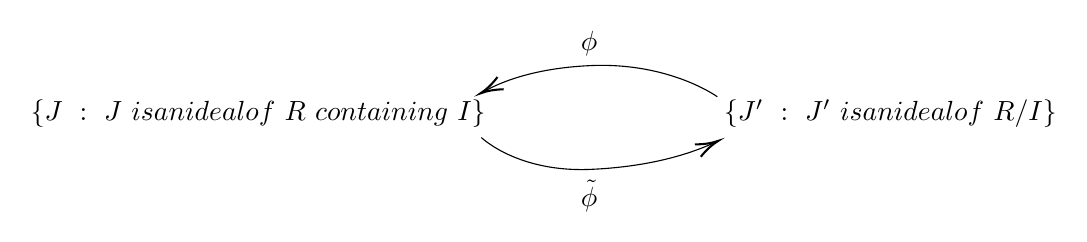
\begin{tikzpicture}[x=0.75pt,y=0.75pt,yscale=-1,xscale=1]
%uncomment if require: \path (0,300); %set diagram left start at 0, and has height of 300

%Curve Lines [id:da8286010344873176] 
\draw    (287.33,184.67) .. controls (288.08,185.42) and (305.5,201.5) .. (340,200) .. controls (372.09,198.61) and (391.3,190.94) .. (399.77,187.06) ;
\draw [shift={(401.5,186.25)}, rotate = 154.61] [color={rgb, 255:red, 0; green, 0; blue, 0 }  ][line width=0.75]    (10.93,-3.29) .. controls (6.95,-1.4) and (3.31,-0.3) .. (0,0) .. controls (3.31,0.3) and (6.95,1.4) .. (10.93,3.29)   ;
%Curve Lines [id:da6236228362848004] 
\draw    (288.6,162.44) .. controls (294.07,159.42) and (309.99,151.31) .. (340,150) .. controls (374.5,148.5) and (396.63,162) .. (401,165) ;
\draw [shift={(286.83,163.42)}, rotate = 333.09] [color={rgb, 255:red, 0; green, 0; blue, 0 }  ][line width=0.75]    (10.93,-3.29) .. controls (6.95,-1.4) and (3.31,-0.3) .. (0,0) .. controls (3.31,0.3) and (6.95,1.4) .. (10.93,3.29)   ;

% Text Node
\draw (69,165) node [anchor=north west][inner sep=0.75pt]    {$\left\{J\ :\ J\ \text{is an ideal of } \ R\ \text{containing} \ I\right\}$};
% Text Node
\draw (403,165) node [anchor=north west][inner sep=0.75pt]    {$\left\{J'\ :\ J'\ \text{is an ideal of } \ R/I\right\}$};
% Text Node
\draw (334,204) node [anchor=north west][inner sep=0.75pt]    {$\tilde{\phi }$};
% Text Node
\draw (334,132) node [anchor=north west][inner sep=0.75pt]    {$\phi $};
\end{tikzpicture}

\(\phi(J') = \pi^{-1}(J')\) and \(\tilde{\phi}(J) = \pi(J)\). We will prove \(\phi\) and \(\tilde{\phi}\) are inverses of each other and if \(J_1' \subseteq J_2'\), then \(\phi(J_1') \subseteq \phi(J_2')\).

Firstly, since \(\pi\) is surjective, \(\pi(\pi^{-1}(J')) = J'\), equivalently, \((\tilde{\phi} \circ \phi)(J') = J'\). For any set map, \( \pi^{-1}(\pi(J)) \supseteq J \) is true. And \( x \in \pi^{-1}(\pi(J)) \) implies \( \pi(x) \in \pi(J) \), which means there is an \( y \in J \) such that  \( \pi(x) = \pi(y) \), which implies \( \pi(x - y) = 0 \), and so \( (x - y) \in \operatorname{ker} \pi = I \subseteq J\). Here \( y \in J \), so is \( x = x - y + y \). Therefore, \( \pi^{-1}(\pi(J)) \subseteq J \), implying \( \pi^{-1}(\pi(J)) = J \), which is equivalent to \((\phi \circ \tilde{\phi})(J) = J\). So \(\phi\) and \(\tilde{\phi}\) are inverses of each other.

Furthermore, let \(x \in \phi(J_1') = \pi^{-1}(J_1')\). Then \(\pi(x) \in J_1' \subseteq J_2'\). So, \(x \in \pi^{-1}(J_2') = \phi(J_2')\). Hence, we have \(\phi(J_1') \subseteq \phi(J_2')\), completing the proof.
    \end{enumerate}
\end{proof}
\begin{definition}
    Let \(R\) be a ring.

    An element \(r \in R\) is called a \emph{zero-divisor} if there is a non-zero \(y \in R\) such that \(r \cdot y = 0\).

    \(R\) is called an \emph{integral domain} if it does not have any non-zero zero-divisors.

An element \(r \in R\) is called \emph{nilpotent} if \(r^n = 0\) for some \(n > 0\).

A \emph{unit} \(r \in R\) is an element that ``divides \(1\)'', i.e., for which there exists \(y \in R, y \neq 0\) such that \(xy = 1\).

\(R\) is a \emph{field} if \(1 \neq 0\) and every non-zero element is a unit.
\end{definition}
\begin{remark}
    \begin{itemize}
        \item \(0\) is also a zero-divisor.
        \item Nilpotent elements are all zero-divisors. To see that, suppose \(r\) is a nilpotent element and \(r^n = 0\). If \(n = 1\), then \(r\) is trivially zero-divisor. Otherwise, we have \(r^{n-1} \in R\) such that \(r \cdot r^{n-1} = 0\).
        \item The set of all units of a ring \(R\) forms an abelian group under multiplication and it is denoted by \(R^\times\).
        \item A unit cannot be a zero-divisor in \(R \neq (0)\). Suppose \(x\) is a unit with \(xy = 1\). If \(x\) is also a zero-divisor, then \(sx = 0\) for some \(s \neq 0\). \[sx = 0 \implies (sx)y = 0y \implies s(xy) = 0 \implies s \cdot 1 = 0  \implies s = 0 \text{ (contradiction!}).\] So,
        \item A field is an integral domain.
    \end{itemize}
\end{remark}
\begin{proposition}
    Suppose \(R\) is a ring and \(R \neq (0)\). Then the following are equivalent:
    \begin{enumerate}
        \item \(R\) is a field.
        \item \(R\) only has two ideals: (0) and \((1)\).
        \item Every homomorphism\footnote{Remember we require \(f(1) = 1\) for a ring homomorphism \(f\).} of \(R\) to a non-zero ring is injective.
    \end{enumerate}
\end{proposition}
\begin{proof}
    \begin{itemize}
        \item (1) \(\implies\) (2). Suppose \(R\) is a field. That means, every non-zero element is a unit. Let \(\mathfrak{a}\) be an ideal of \(R\). If \(\mathfrak{a} = (0)\), we are done. Otherwise, there exists non-zero \(x \in \mathfrak{a} \subseteq R\). Hence, \(x\) is a unit, i.e., there exits \(y \in R\) such that \(xy = yx = 1\). Since \(\mathfrak{a}\) is an ideal, \(y \cdot x \in \mathfrak{a} \implies 1 \in \mathfrak{a} \implies \mathfrak{a} = (1) = R\).

        \item (2) \(\implies\) (3). Suppose \(R\) has only two ideals: \((0)\) and \((1)\). And let \(f: R \longrightarrow S \neq (0)\) be a ring homomorphism. \(\ker f\) is an ideal of \(R\), and it can be either \((0)\) or \((1)\) as per hypothesis. But \(\ker f \neq R\) since we at least have \(1_R \not\in \ker f\) by definition. Hence, \(\ker f = (0)\), which implies \(f\) is injective\footnote{Recall from the first course in algebra: A ring homomorphism is injective iff its kernel is \((0)\).}.
        
        \item (3) \(\implies\) (1). Suppose every homomorphism of \(R\) to a non-zero ring is injective. We want to show that \(R\) is a field, i.e., every non-zero element is a unit. Suppose there is an element \(x \in R\) which is not a unit. Then \((x)\ \neq (1)\) (because if it was \((1)\), then that would mean for some \(y\), \(y \cdot x = 1 \implies x\) is a unit). 

            Consider the canonical projection map \(\pi: R \to R/(x)\) for which \(\ker \pi = (x)\). Since \((x) \neq (1)\), i.e., since \((x) \neq R, R/(x) \neq (0)\). Since \(\pi\) is injective by the hypothesis, so \(\ker \pi = (0)\), which implies \((x) = (0) \implies x = 0\). Hence, the only non-unit in \(R\) is \(0\), and so every non-zero element should be a unit.
    \end{itemize}
\end{proof}


\chapter{Lecture 03}
\hfill {\footnotesize Date: 15/02/2026}
\section{Prime \& Maximal Ideals}
\begin{definition}[Prime Ideal]
    An ideal \(\mathfrak{p}\) in \(R\) is called \emph{prime} if \(\mathfrak{p} \neq (1)\) and if \(xy \in \mathfrak{p}\) implies \(x \in \mathfrak{p}\)  or \(y \in \mathfrak{p}\).   
\end{definition}
\begin{example}
    Take the ring \(R := (\mathbb{Z}, +, \times)\). Then prime ideals of \(R\) are precisely the ideals \((p)\), where \(p\) is prime.

    Because, first of all, every ideal of \(R\) is of the form \((n)\). 

    And we claim that ``\((n)\) is prime ideal iff \(n\) is a prime number;'' 
    equivalently, ``\(\forall a, b \in \mathbb{Z}, ab \in (n) \implies a \in (n) \text{ or } b \in (n)\) iff \(n\) is a prime number;''
 equivalently, ``\(\forall a, b \in Z, n \vert ab \implies n \vert a \text{ or } n \vert b\) iff \(n\) is a prime number.'' We prove that the last statement is indeed true.
    \begin{claim}
        For all \(a, b \in \mathbb{Z}, n \vert ab \implies n \vert a \text{ or } n \vert b\) iff \(n\) is a prime number. 
    \end{claim}
    \begin{proof}[Proof of claim]
        Let for all \(a, b \in \mathbb{Z}, n | ab \implies n | a \text{ or } n | b\). And suppose \(n\) is composite. Then there exists integers \(a'\neq 1, b' \neq 1\) such that \(n = a'b'\). Then \(n = a'b' \big| a' \frac{\text{ lcm}(a', b')}{a'}\) but \(a'b' \not| a'\) and \(a'b' \not| \frac{\text{ lcm}(a', b')}{a'}\), contradicting the hypothesis. Hence, \(n\) must be prime.

        Conversely, let \(n\) be prime. If \(n | a\), we are done. Otherwise, \(n \not| a \implies \operatorname{gcd}(n,a) = 1\), which implies \(px + ay = 1 \implies pbx + aby = b\) for some \(x, y \in \mathbb{Z}\)\footnote{Bezout's identity.}. Since \(p | pbx\) and \(p | (ab)y\)\footnote{since \(p | ab\) by hypothesis.}, therefore \(p | b\).
    \end{proof}
    Therefore, prime ideals in \(\mathbb{Z}\) are principle ideals generated by prime numbers.
\end{example}
\begin{definition}[Maximal Ideal]
    An ideal \(\mathfrak{m}\) in \(R\) is  called \emph{maximal} if \(\mathfrak{m} \neq (1)\) and if there is no ideal \(\mathfrak{a}\) in \(R\) such that \[\mathfrak{m} \subset \mathfrak{a} \subset R \quad \text{(strict inclusion).}\]
    In other words, the only ideal that strictly contains \(\mathfrak{m}\) is \((1)\).
\end{definition}
\begin{proposition}
    \begin{enumerate}
        \item An ideal \(\mathfrak{p}\) is prime if and only if \(R/\mathfrak{p}\) is an integral domain.
        \item An ideal \(\mathfrak{m}\) is maximal if and only if \(R/\mathfrak{m}\) is a field.
    \end{enumerate}
\end{proposition}
\begin{proof}
    \begin{enumerate}
        \item Assume \(\mathfrak{p}\) is a prime ideal. Let \(a+\mathfrak{p}, b+\mathfrak{p} \in R/\mathfrak{p}\) and \((a + \mathfrak{p}) \cdot (b+\mathfrak{p}) = ab + \mathfrak{p}= 0\footnote{It is clear from the context that \(0 \in R/\mathfrak{p}\).}\). \( ab + \mathfrak{p} = 0\) implies \(ab \in \mathfrak{p}\). Since \(\mathfrak{p}\) is prime, \(a \in \mathfrak{p} \implies a+\mathfrak{p} = 0\) or \(b \in \mathfrak{p} \implies b + \mathfrak{p} = 0\). So, only zero-divisor in \(R/\mathfrak{p}\) is \(0\), i.e., \(R/\mathfrak{p}\) is an integral domain.

        Conversely, assume that \(R/\mathfrak{p}\) is an integral domain. Let \(ab \in \mathfrak{p}\). Then \(0 = ab + \mathfrak{p} = (a + \mathfrak{p} )(b + \mathfrak{p})\), which implies that \(a + \mathfrak{p} = 0 \) or \(b + \mathfrak{p} = 0 \), since \(R/\mathfrak{p}\) is an integral domain. Thus, \(a \in \mathfrak{p}\) or \(b \in \mathfrak{p}\) and so \(\mathfrak{p}\) is a prime ideal.

    \item Suppose \(\mathfrak{m}\) is a maximal ideal of \(R\).
        By the \hyperref[proposition:correspondencethm]{Correspondence Theorem}, there is a bijection between the set of ideals 
\(\mathfrak{a}\) of \(R\) containing \(\mathfrak{m}\) and the set of ideals of 
\(R/\mathfrak{m}\).
Since \(\mathfrak{m}\) is maximal, the only ideals of \(R\) containing 
\(\mathfrak{m}\) are: \(\mathfrak{m}\) and \(R\). Therefore, the only ideals 
of \(R/\mathfrak{m}\) are: \((0), (1)\).
Hence, \(R/\mathfrak{m}\) has no nontrivial ideals, so it is a field.

 Conversely, suppose \(R/\mathfrak{m}\) is a field.
Then its only ideals are \((0)\) and \(R/\mathfrak{m}\). By the \hyperref[proposition:correspondencethm]{Correspondence Theorem}, the ideals of \(R/\mathfrak{m}\) correspond bijectively to the ideals 
of \(R\) containing \(\mathfrak{m}\). Therefore, the only ideals of \(R\) 
containing \(\mathfrak{m}\) are: \(\mathfrak{m}\) and \(R\). Hence, 
\(\mathfrak{m}\) is a maximal ideal of \(R\).
    \end{enumerate}
\end{proof}
\begin{corollary}
    Every maximal ideal is prime, but the converse does not hold true.
\end{corollary}
\begin{proof}
    Let \(\mathfrak{m}\) be a maximal ideal in \(R\). Then \(R/\mathfrak{m}\) is a field. Then \(R/\mathfrak{m}\) is an integral domain automatically. Therefore, \(\mathfrak{m}\) is a prime ideal.

    But \((0)\) is a prime ideal in \(\mathbb{Z}\), but not maximal ideal because \((0)\subset (p) \subset (1)\) (strict inclusion).
\end{proof}
\begin{theorem}
    Suppose \(f: R \longrightarrow R'\) is a ring homomorphism, and let \(\mathfrak{p}'\) be a prime ideal in \(R'\). Then, \(f^{-1}(\mathfrak{p}')\) -- the preimage of the ideal is a prime ideal in \(R\).
\end{theorem}
\begin{proof}
    Suppose \(xy \in f^{-1}(\mathfrak{p}')\), which implies \(f(xy) \in \mathfrak{p}'\), and that implies \(f(x)f(y) \in \mathfrak{p}'\), and that implies \(f(x) \in \mathfrak{p}' \text{ or } f(y) \in \mathfrak{p}'\), and that implies \(x \in f^{-1}(\mathfrak{p}') \text{ or } y \in f^{-1}(y)\), which proves \(f^{-1}(\mathfrak{p}')\) is a prime ideal.
\end{proof}
But preimage of a maximal ideal may not be maximal.
\begin{proof}[Counter-example]
    Consider the inclusion map \(\iota: \mathbb{Z} \longrightarrow \mathbb{Q}\). Since \(\mathbb{Q}\) is a field, its only ideals are: \((0)\) and \((1)\). So \((0)\) is a maximal ideal. But \(\iota^{-1}((0)) = (0) \subset (2) \subset (1)\) is not maximal in \(\mathbb{Z}\). 
\end{proof}
\begin{theorem}[Existence of a Maximal Ideal]\label{theorem:maximalidealexistence}
    Every ring \(R \neq (0)\) has at least one maximal ideal.
\end{theorem}
\begin{proof}
    We use Zorn's lemma.
    \begin{theorem}[Zorn's Lemma]
    Let \((S, \le)\) be a non-empty partially ordered set
        \footnote{which means that \(\le\) is a relation on \(S\) satisfying:               \begin{itemize}
                \item \(x \le x\) for all \(x \in S\), 
                \item \(x \le y\) and \(y \le x\) implies \(x = y\) for all \(x, y \in S\),
                \item \(x \le y, y \le z \implies x \le z\) for all \(x, y, z \in S\).
            \end{itemize}
        } (also known as poset). 
        If every chain\footnote{A \textit{chain} in \(S\) is a subset \(C\) of \(S\) such that for any \(x, y \in C\) we have either \(x \le y\) or \(y \le x\).} in \(S\) has an upper bound\footnote{an element \(u\) such that \(x \le u\) for all \(x \in C\)} in \(S\), then \(S\) has at least one maximal element.
    \end{theorem}
    \begin{proof}[Proof of Zorn's lemma]Omitted.\end{proof}
    Let \(\Sigma\) be the set of all ideals \(\mathfrak{a} \neq (1)\) and define partial order \(\subseteq\) using set inclusion. So \((\Sigma, \subseteq)\) is a poset. To apply Zorn's lemma, we need to show that every chain in \((\Sigma, \subseteq)\) has an upper bound in \(\Sigma\).

    Suppose \(\mathcal{C}:= \{\mathfrak{a}_\alpha\}_{\alpha \in J}\) is an arbitrary chain. So \(\mathfrak{a}_\alpha \subseteq \mathfrak{a}_\beta\) or \(\mathfrak{a}_\beta \subseteq \mathfrak{a}_\alpha\) for all \(\alpha, \beta \in J\). Define \[\mathfrak{a} := \bigcup_{\alpha \in J} \mathfrak{a}_\alpha,\] which qualifies as an ideal because \(\mathfrak{a}\) is a subgroup of \(R\) and closed under multiplication by any elements of \(R\):
    \begin{itemize}
        \item \(0 \in \mathfrak{a}_\alpha\) for all \(\alpha \in J\), which implies \(0 \in \mathfrak{a}\).
        \item Suppose \(x, y \in \mathfrak{a}\). So \(x \in \mathfrak{a}_\alpha, y \in \mathfrak{a}_\beta\) for some \(\alpha, \beta \in J\). Since \(\mathfrak{a}_\alpha, \mathfrak{a}_\beta \in \mathcal{C}\), without loss of generality, let \(\mathfrak{a}_\alpha \subseteq \mathfrak{a}_\beta\). Then \(x - y \in \mathfrak{a}_\beta\), implying \(x - y \in \mathfrak{a}\).
        \item Suppose \(r \in R\) and suppose \(x \in \mathfrak{a}\). That means \(x \in \mathfrak{a}_\alpha\) for some \(\alpha \in J\). Hence, \(rx \in \mathfrak{a}_\alpha \subseteq \mathfrak{a}\). 
    \end{itemize}
    Clearly, \(\mathfrak{a}_\alpha \subset \mathfrak{a}\) and \(\mathfrak{a} \in \Sigma\), i.e., every chain in \(\Sigma\) has an upper bound in \(\Sigma\). Therefore, Zorn's lemma implies that \(\Sigma\) has a maximal element. Hence, there is at least one maximal ideal of \(R\).
\end{proof}
\begin{corollary}\label{corollary:primeidealexistence}
    Every ring \(R \neq (0)\) has at least one prime ideal as well.
\end{corollary}
\begin{corollary}\label{corollary:idealcontainedinmaximal}
    If \(\mathfrak{a} \neq (1)\) is an ideal of \(R \neq (0)\), then there exists a maximal ideal \(\mathfrak{m}\) containing \(\mathfrak{a}\).
\end{corollary}
\begin{proof}[Proof 1]
\autoref{theorem:maximalidealexistence} guarantees existence of a maximal ideal \(\mathfrak{m}_q\) in \(R/\mathfrak{a}\). Using \hyperref[proposition:correspondencethm]{Correspondence Theorem}, we have a maximal ideal \(\mathfrak{m}\) such that \[\mathfrak{a} \subseteq \mathfrak{m} \subset R \quad (\text{second inclusion is strict)}.\] 
Maximality of \( \mathfrak{m} \) is guaranteed because the bijection in the correspondence theorem is order-preserving.
\end{proof}
\begin{proof}[Proof 2]
    \todo{To be written...}
\end{proof}
\begin{corollary}\label{corollary:nonunitinmaximalideal}
    Every non-unit of a ring \(R\) is contained in a maximal ideal.
\end{corollary}
\begin{proof}
    Suppose \(x \in R\) is a non-unit. Then \((x) \neq (1)\) because if we had \((x) = (1)\), then there would exist \(y \in R\) such that \(xy = 1\), which contradicts the fact that \(x\) is a non-unit. Using \autoref{corollary:idealcontainedinmaximal}, we conclude that there exists a maximal ideal \(\mathfrak{m}\) such that \(x \in (x) \subset \mathfrak{m}\).
\end{proof}
\section{Local Rings}
\begin{definition}[Local Ring]
    A ring \(R\) is called \emph{local} if it has only one maximal ideal \(\mathfrak{m}\).
\end{definition}
\begin{example}
    \begin{itemize}
        \item All fields are local rings, because a field has only two ideals: \((0)\) and \((1)\), so only maximal is \((0)\).
        \item \(\mathbb{Z}_n\) (also denoted by \(\mathbb{Z}/n\mathbb{Z}\)) is a local ring if and only if \(n = p^a\) for some prime \(p\) and positive integer \(a\).
            \begin{proof}
                
            \end{proof}

%            \begin{proof}
%                It is clear that all the ideals in \(\mathbb{Z}_{p^a}\) are of the form \((n)\), for \(n \in \mathbb{Z}_{p^a}\).
%
%                An ideal \(\mathfrak{a} \subset \mathbb{Z}_{p^a}\) is not equal \((1)\) iff \(n \in \mathbb{Z}_{p^a}\) is a non-unit. It is basic result from number theory that \(u \in \mathbb{Z}_{n}\) is a unit iff \(u\) is co-prime to \(n\), in particular, \(u \in \mathbb{Z}_{p^a}\) is a non-unit iff \(n | p\). Non-units of \(\mathbb{Z}_{p^a}\) are (marked in pink):
%                \[0, 1, \cdots, \colorbox{pink}{\(p\)}, p+1, \cdots, 2p-1, 2p, 2p+1, \cdots, p^2-1, \colorbox{pink}{\(p^2\)}, p^2+1, \cdots, kp^\alpha-1, 
%                \colorbox{pink}{\(kp^\alpha\)}, kp^\alpha+1, \cdots, p^n-1\] for \(\alpha \in \{1, \cdots, n-1\}\) and \(k \in \{1, \cdots, p-1\}\).


%            \end{proof}
    \end{itemize}
\end{example}
\todo{To be written...}
\begin{nonexample}
    \(\mathbb{Z}\) is not a local ring because all prime ideals are maximal in \(\mathbb{Z}\), and there are more than \( 1 \) prime ideal in  \( \mathbb{Z} \).
\end{nonexample}
\begin{definition}[Semi-local Ring]
    A ring \(R\) is called \emph{semi-local} if number of maximal ideals in \(R\) is finite.
\end{definition}
\begin{example}
    \(Z_n\) is always semi-local since its number of ideals is finite, so is number of maximal ideals.
\end{example}
\begin{exercise}
    Is \(\mathbb{K}[x]\) local? When is \(\mathbb{K}[x]/(x^n)\) local?

\end{exercise}


\chapter{Lecture 04}\label{Lec04}
\hfill {\footnotesize \textit{Date: 23/02/26}}
\section{Rings of Fractions}
The procedure by which one constructs the rational field \(\mathbb{Q}\) from the ring of integers \(\mathbb{Z}\) (and embeds \(\mathbb{Z}\) in \(\mathbb{Q}\)) extends easily to any integral domain \(R\) and produces the \emph{field of fractions} of \(R\).
\begin{definition}[Field of Fractions]
 Let \( R \) be an integral domain. Define an equivalence relation \(\sim\) on \(R \times R \smallsetminus \{0\}\) by:
\[
(a, b) \sim (c, d) \iff ad - bc = 0.
\] 
Let \(a/b\) denote the set of equivalence class of \((a,b)\). We put a field structure on \(R \times R \smallsetminus \{0\}/\sim\) --- the set of equivalence classes under the relation \(\sim\), by defining addition and multiplication of these ``fractions'' \(a/b\) in the same way as in \(\mathbb{Q}\), that is,  
\[
a/b + c/d := (ad + bc)/bd.
\]  
\[
a/b \cdot c/d := ac/bd.
\] 
The ``field'' \((R \times R \smallsetminus \{0\}/\sim, +, \cdot)\) is called the \emph{field of fractions} of \(R\).
\end{definition}

Now we have to check that (1) \(\sim\) is an equivalence relation, (2) the operations defined above are well-defined, and (1) field of fractions of  \(R\) is indeed a field:
\begin{enumerate}[label=\arabic*)]
    \item \textbf{Reflexive:} \(a/b \sim a/b\) as  \(ab - ab = 0\).

        \textbf{Symmetric:} \((a,b) \sim (c,d) \Longrightarrow ad - bc = 0 \Longrightarrow -(ad - bc) = cb - da = 0 \Longrightarrow (c,d) \sim (a,b)\).

        \textbf{Transitive:}\((a,b) \sim (c, d)\) and  \((c,d) \sim (e,f)\)

        \(\Longrightarrow ad - bc = 0\) and \(cf - ed = 0\) 

        \(\Longrightarrow (ad - bc)f = 0\) and \(b(cf - ed) = 0\) 

        \(\Longrightarrow adf - bcf = 0\) and \(bcf - bed = 0\)

         \(\Longrightarrow adf - bed = 0\) 

         \(\Longrightarrow (af - be) d = 0\)

         Since \(R\) is an integral domain and \(d \in R \smallsetminus \{0\}\),  so \(d\) is not a zero-divisor. So \(af - be = 0\), implying  \((a,b) \sim (e,f)\).
    \item Tedious. 
    \item Tedious. 
\end{enumerate}
This generalisation only works if \(R\) is an integral domain, because the verification that  \(\sim\) is transitive involves canceling, i.e., the fact that  \(R\) has no non-zero zero divisor. However, there is a way around:

A \emph{multiplicatively closed subset} of a ring \(R\) is a subset  \(S\) of  \(R\) such that  \(1 \in S\) and  \(S\) is closed under multiplication: in other words,  \(S\) is a sub-monoid of the multiplicative monoid of  \(R\). One obvious way to construct such a set is taking an element \( f \in R \). Then  the set \( \{1, f, f^2, f^3, \ldots\} \) is a multiplicatively closed subset of \( R \).

\begin{definition}[Ring of Fractions]
 Let \( R \) be any ring, and \(S\) be a multiplicatively closed subset of it. Define an equivalence relation \(\sim\) on \(R \times S\) by:
\[
    (a, s) \sim (b, t) \iff (at - bs)u = 0 \text{ for some } u \in S.
\] 
Let \(a/s\) denote the set of equivalence class of \((a,s)\), and let \(S^{-1}R\) denote the set of equivalence classes under the relation \(\sim\). We put a ring structure on \(S^{-1}R\) by defining addition and multiplication of these ``fractions'' \(a/s\) in the same way as in elementary algebra, that is,  
\[
a/s + b/t := (at + bs)/st.
\]  
\[
a/s \cdot b/t := ab/st.
\] 
The ``ring'' \((S^{-1}R, +, \cdot)\) is called the \emph{ring of fractions} of \(R\) with respect to \(S\).
\end{definition}
We now verify (1) \(\sim\) is an equivalence relation, (2) operations  \(+\) and  \(\cdot\) are well-defined, and (3)  \(S^{-1}R\) is a (commutative) ring (with identity):
\begin{enumerate}[label=\arabic*)]
    \item Proof of reflexivity and symmetry of \(\sim\) follows as before. We now show it is transitive:
        \((a, s) \sim (b, t)\) and  \((b, t) \sim (c, u)\)

        \(\Longrightarrow (at - bs)u = 0\) and \((bu - ct)w = 0\) for some \(u,w \in S\) 

        \(\Longrightarrow (at - bs)v = 0\) and \((bu - ct)w = 0\) for some \(v,w \in S\) 

\(\Longrightarrow atv - bsv = 0\) and \(buw - ctw = 0\) for some \(v,w \in S\) 

\(\Longrightarrow atvuw - bsvuw = 0\) and \(buwvs - ctwvs = 0\) for some \(v,w \in S\)

\(\Longrightarrow atvuw - ctwvs = 0\) for some \(v, w \in S\)

 \(\Longrightarrow (au - cs) tvw\), where \(tvw \in S\), as  \(S\) is multiplicatively closed.

Hence, \((a, s) \sim (c,u)\). Therefore,  \(\sim\) is indeed an equivalence relation.
    \item Tedious.
    \item Tedious.
\end{enumerate}
\begin{remark}
    Every element \( \frac{s}{t} \in S^{-1}R \), where \( s \in S \) is invertible.
\end{remark}
\begin{example}
    Take \( R = \mathbb{Z} \), and \( S = \{1, 6, 6^2, 6^3, \ldots\} \). Then 
    \[
        S^{-1}R = \left\{\frac{a}{6^k} \mid a \in \mathbb{Z} \smallsetminus (S \smallsetminus \{1\}), k \in \mathbb{Z}_{k \ge 0}\right\}.
    \]
\end{example}
Another example:
\begin{example}
    Take \( R = \mathbb{K}[x] \). Then
     \begin{enumerate}
         \item First take \( S = \mathbb{K} \smallsetminus \{0\}\). Then \( S^{-1}\mathbb{K}[x] \) is the set of all rational functions over  \( \mathbb{K} \). 
         \item Take  \( S = \{1, x, x^2, x^3, \ldots\} \). Then \( S^{-1}\mathbb{K}[x] = \mathbb{K}[x, x^{1}] \) is the  \emph{Laurent polynomial ring} over \( \mathbb{K} \).
    \end{enumerate}
\end{example}
We now discuss the concept of \emph{localisation} of a ring  \(R\) about a prime ideal  \(\mathfrak{p}\):
\begin{lemma}
    Let \(\mathfrak{p}\) be a prime ideal of \(R\). Then  \(R \smallsetminus \mathfrak{p}\) is a multiplicatively closed set.

    In fact, \(R \smallsetminus \mathfrak{p}\) is multiplicatively closed iff \(\mathfrak{p}\) is prime.
\end{lemma}
\begin{proof}
   Since \(\mathfrak{p}\) is prime, \(1 \not\in \mathfrak{p}\). So \(1 \in R \smallsetminus \mathfrak{p}\).

   Let \(x, y \in R \smallsetminus \mathfrak{p}\), i.e., \(x,y \not\in \mathfrak{p}\). If \(xy \not\in R \smallsetminus \mathfrak{p}\), then \(xy \in \mathfrak{p}\), which implies \(x \in \mathfrak{p}\) or \(y \in \mathfrak{p}\), which is a contradiction. Hence, \(xy \not\in  \mathfrak{p}\), i.e., \(xy \in R \smallsetminus \mathfrak{p}\).
\end{proof}
\begin{theorem}[Localisation]
    Let \(\mathfrak{p}\) be a prime ideal of \(R\), and let \(S = R \smallsetminus \mathfrak{p}\). Then \(R_\mathfrak{p} \coloneq S^{-1}R\) is a local ring.

    The process of passing from \(R\) to  \(R_\mathfrak{p}\) is called \emph{localisation}.
\end{theorem}
\begin{proof}
    Let \(\mathfrak{m} \coloneq \{a/s \in R_\mathfrak{p} \mid a \in \mathfrak{p}\}\). We claim \(\mathfrak{m}\) is the only maximal ideal of \(R_\mathfrak{p}\).

We first prove \(\mathfrak{m}\) is an actually an ideal: \(0/s \in R_\mathfrak{p}\) because \(0 \in \mathfrak{p}\). If \(a/s, b/t \in \mathfrak{m}\), then \((at+bs)/st \in \mathfrak{m}\) because \(a, b \in \mathfrak{p}\), so is \(at + bs\). Furthermore, if \(a/s \in \mathfrak{m}\) and \(b/t \in R_\mathfrak{p}\), then \(ab/st \in \mathfrak{m}\) as \(a \in \mathfrak{p}\), so is \(ab\).

Now, 
\end{proof}
\todo{To be written}
\begin{remark}
    If \(R\) is an integral domain and  \(S = R \smallsetminus \{0\}\), then \(S^{-1}R\) is just the field of fractions of  \(R\).
\end{remark}

The procedure of localisation of a ring gives tones of examples of local rings since every ring can be localised because every ring has at least one prime ideal (\autoref{corollary:primeidealexistence}).
\begin{example}
    Take \( R = \mathbb{Z} \). And a prime ideal \( (p) \) of  \( \mathbb{Z} \). Then \( S = \mathbb{Z} \smallsetminus (p) \) is a multiplicatively closed subset of \( \mathbb{Z} \). 
    \[
        \mathbb{Z}_{(p)} = S^{-1}\mathbb{Z} = \left\{\frac{a}{b} \mid a \in \mathbb{Z}, b \in \mathbb{Z}, p \nmid b\right\}.
    \] 
\end{example}
\section{Local Rings -- Again}
\begin{theorem}
    A ring \(R\) is local if and only if all the non-units form an ideal. 
\end{theorem}
To illustrate usefulness of this theorem, consider \(\mathbb{Z}\). Units of \(\mathbb{Z}\) are: \(-1, 1\). So the set of all non-units is  \(\{\ldots, -3, -2, 0, 2, 3, \ldots\}\), which is not an ideal. So, \(\mathbb{Z}\) is not a local ring!
\begin{proof}[Proof of theorem]
    (\( \implies \)) Let \( R \) be a local ring, i.e., it has only one maximal ideal, call it \( \mathfrak{m} \). We have to show that all non-units in  \( R \) form an ideal

    If \( \mathfrak{m} \) contains all the non-units, then we are done. Otherwise, let \( x \in R \) be a non-unit that is not contained in  \( \mathfrak{m} \). Then there exists maximal ideal other than \( \mathfrak{m} \) that contains \( x \), which is contradiction, since  \( R \) has only one maximal ideal. So, all non-units in \( R \) are contained in \( \mathfrak{m} \), thus, all non-units form an ideal, namely, \( \mathfrak{m} \).

    (\( \Longleftarrow \)) Suppose all the non-units in \( R \) form an ideal, call it, \( \mathfrak{m} \). We have to show that \( \mathfrak{m} \) is the only maximal ideal of \( R \).

    First of all, \( \mathfrak{m} \) is maximal, because if \( \mathfrak{a} \) is an ideal other than \( \mathfrak{m} \) that contains  \( \mathfrak{m} \), then it has to contain a unit, so  \(  \mathfrak{a} = R \). So \( \mathfrak{m} \) is maximal. If there is another maximal ideal \( \mathfrak{m'} \) in \( R \), then there exists \( x \in \mathfrak{m'} \smallsetminus \mathfrak{m} \). Then it implies that \( x \) is a unit, so  \( \mathfrak{m'} = R\), which is a contradiction. Hence, \( \mathfrak{m} \) is the only maximal ideal in \( R \).
\end{proof}
\begin{theorem}
    Let \(R\) be a ring and let  \(\mathfrak{m}\) be a maximal ideal --- such that every element of \(1 + \mathfrak{m} = \{1 + m  \mid  m \in \mathfrak{m}\} \) is a unit. Then \(R\) is a local ring. 
\end{theorem}
\begin{proof}
    Since \( \mathfrak{m} \) is a maximal ideal and \( \mathfrak{m} \neq (1) \), we have \( 1 \notin \mathfrak{m} \), and \( \mathfrak{m} \) contains no units.

Suppose \( x \notin \mathfrak{m} \), i.e., \( x \in R \smallsetminus \mathfrak{m} \). Consider the ideal generated by \( x \) and \( \mathfrak{m} \); call it \( \mathfrak{a} \). Then \( \mathfrak{m} \subset \mathfrak{a} \) (strictly included since \( x \in \mathfrak{a} \) but \( x \notin \mathfrak{m} \)). By maximality of \( \mathfrak{m} \), we must have \( \mathfrak{a} = (1) \).

Since \( \mathfrak{a} \) is generated by \( x \) and \( \mathfrak{m} \), a generic element of \( \mathfrak{a} \) is of the form
\[
x y + t \quad \text{where } y \in R,\ t \in \mathfrak{m}.
\]
Because \( 1 \in \mathfrak{a} \), there exist \( y \in R \) and \( t \in \mathfrak{m} \) such that
\[
x y + t = 1.
\]
Then
\[
x y = 1 - t = 1 + (-t) \in 1 + \mathfrak{m}.
\]
By hypothesis, every element of \( 1 + \mathfrak{m} \) is a unit, so \( x y \) is a unit. Hence there exists \( u \in R \) such that \( (x y) u = 1 \), i.e., \( x (y u) = 1 \). Therefore \( x \) is a unit.

Thus every element not in \( \mathfrak{m} \) is a unit, and so \( \mathfrak{m} \) consists of all non-units. Hence \( R \) is a local ring (by the previous theorem).
\end{proof}
\section{Nilradicals \& Jacobson Radicals}
\begin{definition}[Nilradical]
    The set \(\mathfrak{N}\) of all nilpotent elements in a ring is called the \emph{nilradical} of that ring.
\end{definition}
\begin{proposition}
    The nilradical of a ring is an ideal.
\end{proposition}
\begin{proof}
    Suppose \(R\) is a ring and \(\mathfrak{N} = \{x \in R : x^n=0 \text{ for some } n > 0\}\) is the nilradical. We want to show that \(\mathfrak{N}\) is an ideal, i.e., \(\mathfrak{N}\) satisfies subgroup criterion and \(\mathfrak{N}\) is closed under multiplication by any elements of \(R\):

    \begin{itemize}
        \item \(0 \in \mathfrak{N}\) clearly. And let \(x, y \in \mathfrak{N}\). Then \(x^k = 0\) and \(y^n = 0\) for some \(k, n > 0\). 
            \[(x-y)^{k+n+1} = \sum_{i = 0}^{k+n+1}C_i \cdot x^r y^s \quad\text{ where } r+s = k + n + 1.\]

            Now, notice that for any particular term in this expansion, it can not be the case that both \(r < k\) and \(s < n\) are true. So for each term either \(r \ge k\) or \(s \ge n\). So every term in \((x-y)^{k+n+1}\) is actually \(0\). So \((x-y)^{k+n+1} = 0\), implying \(x - y \in \mathfrak{N}\).
        \item Let \(x \in \mathfrak{N}\) and let \(r \in R\). Then \(x^k = 0\) for some \(k > 0\). So \[(rx)^k = r^kx^k = r^k \cdot 0 = 0 \implies rx \in \mathfrak{N}.\]
    \end{itemize}
    Hence, \(\mathfrak{N}\) is an ideal \(R\).
\end{proof}
\begin{lemma}
    Suppose \(R\) is a ring and \(\mathfrak{N}\) be the nilradical of \(R\) which is an ideal. Then \(R/\mathfrak{N}\) only has one nilpotent element, namely \(0 + \mathfrak{N}\).
\end{lemma}
\begin{proof}
    Let \(x + \mathfrak{N}\) be a nilpotent element of \(R/\mathfrak{N}\). Then there exists integer \(k > 0\), such that 
    \[
        \left(x + \mathfrak{N}\right)^k = x^k + \mathfrak{N} = 0 + \mathfrak{N}
    \]
    Then \(x^k \in \mathfrak{N}\). So there exists integer \(n > 0\), such that  \(x^{kn} = 0\), which implies  \(x \in \mathfrak{N}\). So, \(x + \mathfrak{N} = 0 + \mathfrak{N}\). Since, it is true for any \(x \in R\), that means any nilpotent element of \(R/\mathfrak{N}\) is of the form \(0 + \mathfrak{N}\), which implies \(R/\mathfrak{N}\) has only one nilpotent element, namely, \(0 + \mathfrak{N}\).
\end{proof}
\begin{proposition}
    Nilradical \(\mathfrak{N}\) of a ring \(R\) is the intersection of all prime ideals in \(R\).
    \[
        \mathfrak{N} = \bigcap_{\substack{\mathfrak{p} \text{ prime} \\ \text{in } R}} \mathfrak{p}.
    \] 
\end{proposition}
\begin{proof}
    We prove the two inclusions separately.

    \begin{enumerate}[label=\textit{Step} \arabic*., leftmargin=*]

\item \(\mathfrak{N} \subseteq \bigcap_{\mathfrak{p} \text{ prime}} \mathfrak{p}\):  
    Let \(f \in \mathfrak{N}\). Then \(f^n = 0\) for some \(n > 0\). Let \(\mathfrak{p}\) be any prime ideal of \(R\). Since \(0 \in \mathfrak{p}\), we have \(f^n = 0 \in \mathfrak{p}\). Because \(\mathfrak{p}\) is prime, \(f \in \mathfrak{p}\) or \(f^{n-1} \in \mathfrak{p}\). Repeating this argument, we eventually conclude \(f \in \mathfrak{p}\). Hence \(f\) belongs to every prime ideal \(\mathfrak{p}\), i.e., \(\bigcap_{\mathfrak{p} \text{ prime}} \mathfrak{p} \).

\item \(\bigcap_{\mathfrak{p} \text{ prime}} \mathfrak{p} \subseteq \mathfrak{N}\):  
We prove the contrapositive: if \(f \notin \mathfrak{N}\), then there exists a prime ideal \(\mathfrak{p}\) such that \(f \notin \mathfrak{p}\).

Suppose \(f \notin \mathfrak{N}\). Then \(f^n \neq 0\) for all \(n > 0\). Consider the set
\[
    \Sigma = \{ \mathfrak{a} \subset  R \text{ ideal} \mid f^n \notin \mathfrak{a} \text{ for all } n > 0 \}.
\]
Since \(f^n \neq 0\) for all \(n\), \(f^n \not\in (0)\) for all \(n > 0\). Therefore, \((0) \in \Sigma\), and so \(\Sigma\) is nonempty.

Partially order \(\Sigma\) by set-inclusion. If \((\mathfrak{a}_\alpha)_{\alpha \in \mathcal{A}}\) is a chain in \(\Sigma\), then \(\bigcup_{\alpha \in \mathcal{A}} \mathfrak{a}_\alpha\) is an ideal (one checks easily) and, because \(f^n \notin \mathfrak{a}_\alpha\) for all \(\alpha\) and all \(n\), we have \(f^n \notin \bigcup_{\alpha} \mathfrak{a}_\alpha\) for all \(n\). Hence \(\bigcup_{\alpha} I_\alpha \in \Sigma\) and is an upper bound for the chain.

By Zorn's Lemma, \(\Sigma\) has a maximal element, call it \(\mathfrak{p}\). Since \(\mathfrak{p}\) is a maximal ideal\todo{But it not be maximal in \( R \), rest of the proof needs correction.}, so \(\mathfrak{p}\) is also a prime ideal. So we have found a prime ideal \(\mathfrak{p}\) that does not contain \(f^n\) for all  \(n > 0\), in particular,  \(f \not\in \mathfrak{p}\).

Hence \(f \notin \bigcap_{\mathfrak{p} \text{ prime}} \mathfrak{p}\), completing the proof.
\end{enumerate}
\end{proof}
\begin{definition}[Jacobson Radical]
    The intersection of all the maximal ideals is called the \textit{Jacobson radical}, denoted by \(\mathfrak{R}\).
    \[
        \mathfrak{R} \coloneq \bigcap_{\substack{\mathfrak{m} \text{ maximal} \\ \text{in } R}} \mathfrak{m}.
    \] 
\end{definition}
It is always true that \(\mathfrak{R} \subseteq \mathfrak{N}\). In extreme cases, we have \(\mathfrak{R} = \mathfrak{N}\).
\begin{theorem}[Characterisation of Jacobson Radical]\label{thm:characterisationOfJacobsonRad}
    \(x \in \mathfrak{R}\) if and only if \(1 - xy\) is a unit for all  \(y \in R\).
\end{theorem}
\begin{proof}
\((\Longrightarrow)\) We will prove the equivalent contrapositive statement: if \(1 - xy\) is not a unit for some  \(x \in R\), then  \(x \not\in \mathfrak{R}\).

If \(1 - xy\) is not a unit for some \(y \in R\); then there exists a maximal  \(\mathfrak{m}\), that contains \(1 - xy\) (\autoref{corollary:nonunitinmaximalideal}). Since  \(x \in \mathfrak{R}\), so \(x \in \mathfrak{m}\), and \(xy \in \mathfrak{m}\) as well. Then we also have \((1-xy)+xy  = 1\in \mathfrak{m}\), which leads to a contradiction as maximcal ideal cannot contain \(1 \in R\). So forward direction follows.

 \((\Longleftarrow)\) Again we prove equivalent contrapositive statement: if \(x \not\in  \mathfrak{R}\), then \(1-xy\) is not a unit for some  \(y \in R\).

\(x \not\in \mathfrak{\mathfrak{R}}\), so there is a maximal ideal \(\mathfrak{m}\) that does not contain \(x\). Since \(x \not\in \mathfrak{m}\) --- a maximal ideal, the ideal generated by \(\mathfrak{m}\) and \(x\) is \((1)\). That means for some \( y \in R \) and \( t \in \mathfrak{m} \), we must have \(xy + t = 1\), which means  \(t = 1 - xy \in \mathfrak{m}\). Since \(\mathfrak{m} \neq (1)\),  \(1 - xy\) can not be unit for that particular  \(y \in R\), completing the proof. 
\end{proof}


\chapter{Lecture 05}\label{section:lec05pt1}
\hfill {\footnotesize \textit{Date: 25/02/2026 (Part 1)}}
\section{Operations on Ideals}
We can define various operations on ideals:
\begin{definition}[Sum of two ideals]
    Suppose \(\mathfrak{a}\) and \(\mathfrak{b}\) are ideals in a ring \(R\). Their \emph{sum} \(\mathfrak{a}+\mathfrak{b}\) is defined as
    \[
        \mathfrak{a} + \mathfrak{b} := \{a + b \mid a \in \mathfrak{a}, b\in \mathfrak{b}\}.
    \]
\end{definition}
It is very easy to check that \(\mathfrak{a} + \mathfrak{b}\) is an ideal:

    Firstly, \(0 \in \mathfrak{a}\) and \(0 \in \mathfrak{b}\). So, \(0+0 = 0 \in \mathfrak{a} + \mathfrak{b}\). Let \(a_1 + b_1, a_2+b_2 \in \mathfrak{a} + \mathfrak{b}\) with \(a_1, a_2 \in \mathfrak{a}\) and \(b_1, b_2 \in \mathfrak{b}\). Then \((a_1 - a_2) \in \mathfrak{a}\) and \((b_1-b_2) \in \mathfrak{b}\). So it follows that 
        \[(a_1 + b_1) - (a_2+b_2) = (a_1 - a_2) + (b_1 - b_2) \in \mathfrak{a} + \mathfrak{b}, \] Therefore,  \(\mathfrak{a} + \mathfrak{b}\) is a subgroup of \(R\). 

    Furthermore, if \(a + b \in \mathfrak{a} + \mathfrak{b}\) with \(a \in \mathfrak{a}\) and \(b \in \mathfrak{b}\), then for any \(r \in R\), we have \(ra \in \mathfrak{a}\) and \(rb \in \mathfrak{b}\), which implies \(rx + ry = r(x+y) \in \mathfrak{a} + \mathfrak{b}\). So, \(\mathfrak{a} + \mathfrak{b}\) is closed under multiplication by ring elements.
    \begin{example}\label{example:mplusnequalgcd}
    Consider the ring \((\mathbb{Z}, +, \times)\). Then \((m) + (n) = \text{gcd(m, n)}\).

    To prove that, let \(d = (\text{gcd}(m,n))\). Since \(d | m, n\), therefore, \(d | mx + ny\) for all \(x, y \in \mathbb{Z}\). So \[(m) + (n) = \{mx + ny \mid x, y \in \mathbb{Z}\} \subseteq (d).\]
    Conversely, take \(x \in (d)\). Then \(x = dk\) for some \(m \in \mathbb{Z}\). By Bezout's identity, there exists \(x, y \in \mathbb{Z}\) such that \[d = mx + ny \implies dk = m(xk) + n(yk) \in (m)+(n).\]
    Hence, \((d) \subseteq (m) + (n)\), completing the proof.
\end{example}
\begin{proposition}
    \(\mathfrak{a}+\mathfrak{b}\) is the smallest ideal that contains both \(\mathfrak{a}\) and \(\mathfrak{b}\).
\end{proposition}
\begin{proof}
    We want to show that if \(\mathfrak{c}\) is an ideal containing both \(\mathfrak{a}\) and \(\mathfrak{b}\), then \(\mathfrak{c}\) contains \(\mathfrak{a}+\mathfrak{b}\).

    Take \(a + b \in \mathfrak{a} + \mathfrak{b}\) with \(a \in \mathfrak{a}\) and \(b \in \mathfrak{b}\). Then \(a \in \mathfrak{a} \subseteq \mathfrak{c}\) and \(b \in \mathfrak{b} \subseteq \mathfrak{c}\). Since \(\mathfrak{c}\) is an ideal, we have \(a+b \in \mathfrak{c}\), implying, \(\mathfrak{c}\) contains \(\mathfrak{a}+\mathfrak{b}\).
\end{proof}
More generally, we can define the following:
\begin{definition}[Sum of a collection of ideals]
    Let \(\{\mathfrak{a}_\alpha\}_{\alpha \in \mathcal{A}}\) be an arbitrary collection of ideals in \(R\). We can define the \emph{sum}
    \[\sum_{\alpha \in \mathcal{A}} \mathfrak{a}_\alpha \coloneq \left\{\sum_{\alpha \in \mathcal{A}} a_\alpha \mid a_\alpha \in \mathfrak{a}_\alpha \text{ and } a_\alpha = 0 \text{ for all but finitely many } \alpha \in \mathcal{A}\right\}.\]
\end{definition}
It is straightforward to check that this is indeed an ideal, and that it is the smallest ideal of \(R\) that contains \(\mathfrak{a}_\alpha\) for all \(\alpha \in \mathcal{A}\).
\begin{remark}
In this definition, we allowed only finitely many terms to be nonzero; because no topology has been defined on the set of ideals, so we cannot discuss the convergence of an infinite sum.
\end{remark}

\begin{definition}[Interseciton]
    Let \(\{\mathfrak{a}_\alpha\}_{\alpha \in \mathcal{A}}\) be an arbitrary collection of ideals in \(R\). Then \emph{intersection} \[\bigcap_{\alpha \in \mathcal{A}}\mathfrak{a}_\alpha\] is also an ideal.
\end{definition}
The proof that \(\bigcap_{\alpha \in \mathcal{A}}\mathfrak{a}_\alpha\) is an ideal is very straightforward:

Firstly, for all \(\alpha \in \mathcal{A}\), \(0 \in \mathfrak{a}_\alpha\), so \(0 \in \bigcap_{\alpha \in \mathcal{A}}\mathfrak{a}_\alpha\). Moreover, take \(x, y \in \bigcap_{\alpha \in \mathcal{A}}\mathfrak{a}_\alpha\). Then for all for all \(\alpha \in \mathcal{A}\), \(x, y \in \mathfrak{a}_\alpha\), implying \(x-y \in \mathfrak{a}_\alpha\). Hence, \(x-y \in \bigcap_{\alpha \in \mathcal{A}} \mathfrak{a}_{\alpha}\).

Furthermore, suppose \(r \in R\), and \(x \in \bigcap_{\alpha \in \mathcal{A}} \mathfrak{a}_{\alpha}\). Then for all \(\alpha \in \mathcal{A}, x \in \mathfrak{a}_\alpha\), implying \(rx \in \mathfrak{a}_\alpha\). Thus \(rx \in \bigcap_{\alpha \in \mathcal{A}} \mathfrak{a}_{\alpha}\).

\begin{example}\label{mcapnequalslcm}
    Again, consider the ring \((\mathbb{Z}, +, \times)\). \((m) \cap (n) = (\text{lcm}(m, n))\).

    To show that, let \(l = \text{lcm}(m, n)\). Since \(l\) is multiple of both \(m, n\), we have \((l) \subseteq (m)\) and \((l) \subseteq (n)\). Hence, \(l \subseteq (m) \cap (n)\).

    Conversely, let \(k \in (m) \cap (n)\). Then \(m\) and \(n\) both divides \(k\).
    \begin{claim}
        If \(m | k\) and \(n | k\), then \(l = \text{lcm}(m,n) | k\). 
    \end{claim}
    \begin{proof}
        Write the prime factorizations
\[
m=\prod P_i^{a_i}, 
\quad 
n=\prod P_i^{b_i}, 
\quad 
k=\prod P_i^{c_i}.
\]
Since $m |k$ and $n | k$, we have $a_i \le c_i$ and $b_i \le c_i$ for all $i$.
Thus
\[
\operatorname{lcm}(m,n)=\prod P_i^{\max(a_i,b_i)}.
\]
Because $\max(a_i,b_i)\le c_i$ for all $i$, it follows that
\[
\operatorname{lcm}(m,n)| k.
\]
    \end{proof}
    So \(\text{lcm}(m,n) | k\), which implies \(k \in (\text{lcm}(m,n))\). So \((m)\cap (n) \subseteq (l)\).

    Therefore, \((m) \cap (n) = (l) = (\text{lcm}(m,n))\).
\end{example}
\begin{definition}[Product of Two Ideals]
    Suppose \(\mathfrak{a}, \mathfrak{b}\) are two ideals in \(R\). Then their \emph{product} \(\mathfrak{a}\mathfrak{b}\) is defined as \[\mathfrak{a}\mathfrak{b} \coloneq \left\{\sum_{\alpha \in \mathcal{A}} a_\alpha b_\alpha \mid a_\alpha \in \mathfrak{a}, b_\alpha \in \mathfrak{b} \text{ and } a_\alpha b_\alpha = 0 \text{ for all but finitely many } \alpha \in \mathcal{A} \right\}.\]
\end{definition}
We now check that \(\mathfrak{a}\mathfrak{b}\) is indeed an ideal: 

Firstly, \(0 \in \mathfrak{a}\) and \(0 \in \mathfrak{b}\). So \(0 \cdot 0 = 0 \in \mathfrak{a}\mathfrak{b}\). Moreover, suppose \(\sum_{\alpha \in \mathcal{A}} a_\alpha b_\alpha, \sum_{\beta \in \mathcal{B}} a_\beta' b_\beta' \in \mathfrak{ab}\) where \(a_\alpha, a_\beta' \in \mathfrak{a}\) and \(b_\alpha, b_\beta' \in \mathfrak{b}\), and let \(\mathcal{C} = \mathcal{A} \sqcup \mathcal{B}\) be the \href{https://math.stackexchange.com/questions/1631396/what-is-the-difference-between-disjoint-union-and-union}{disjoint union} of \(\mathcal{A}, \mathcal{B}\).

Then \[
    \sum_{\alpha \in \mathcal{A}} a_\alpha b_\alpha - \sum_{\beta \in \mathcal{B}} a_\beta' b_\beta' = \sum_{\alpha \in \mathcal{A}} a_\alpha b_\alpha + \sum_{\beta \in \mathcal{B}} (-a_\beta') b_\beta' = \sum_{\gamma \in \mathcal{C}} a_\gamma'' b_\gamma'',
\]
where \(a_\gamma'' = \begin{cases}
    a_\alpha &\text{if } \gamma \in \mathcal{A}\\
    -a_\beta' &\text{if } \gamma \in \mathcal{B}
\end{cases}\) and \(b_\gamma'' = \begin{cases}
    b_\alpha &\text{if } \gamma \in \mathcal{A}\\
    b_\beta' &\text{if } \gamma \in \mathcal{B}
\end{cases}\). And clearly, \(a_\gamma'' \in \mathfrak{a}\) and \(b_\gamma'' \in \mathfrak{b}\), and \(a_\gamma''b_\gamma'' = 0\) for all but finitely many  \(\gamma \in \mathcal{C}\).

Furthermore, suppose \(r \in R\), and \(\sum_{\alpha \in \mathcal{A}} a_\alpha b_\alpha \in \mathfrak{ab}\) with \(a_\alpha \in  \mathfrak{a}, b_\alpha \in \mathfrak{b}\). Then \(ra_\alpha \in  \mathfrak{a}\) as well. Since the sum is finite, we can use repeated distributive law of ring \(R\) to write 
\[
    r \left(\sum_{\alpha \in \mathcal{A}} a_\alpha b_\alpha\right) = \sum_{\alpha \in \mathcal{a}} r (a_\alpha b_\alpha) =  \sum_{\alpha \in \mathcal{a}} (r a_\alpha) b_\alpha, \text{ where } ra_\alpha \in \mathfrak{a}, b_\alpha \in \mathfrak{b}.
\]

This definition can be generalised to finitely many ideals:
\begin{definition}[Product of Finitely Many Ideals]
    Suppose \(\{\mathfrak{a}_1, \cdots, \mathfrak{a}_n\}\) is a finite collection of ideals in a ring \(R\). Then
    \[
        \mathfrak{a_1}\cdots \mathfrak{a}_n \coloneq  \left\{\sum_{\alpha \in \mathcal{A}} a_{1_\alpha }\cdots a_{n_\alpha } \mid a_{k_\alpha } \in \mathfrak{a}_k \text{ and } a_{1_\alpha }\cdots a_{n_\alpha } = 0 \text{ for all but finitely many } \alpha \in \mathcal{A} \right\}.
        \]
\end{definition}
Multiplication distributes over sum. 
\begin{lemma}[Distributivity for Product and sum] 
\(\mathfrak{c} (\mathfrak{a} + \mathfrak{b}) = \mathfrak{c}\mathfrak{a} + \mathfrak{cb}\) for ideals \(\mathfrak{a}, \mathfrak{b}, \mathfrak{c}\) in ring \(R\).
\end{lemma}
\begin{proof}
    Suppose \(x \in \mathfrak{c}(\mathfrak{a}+\mathfrak{b})\) Then \(x = \sum_{\alpha \in \mathcal{A}} c_\alpha (a_\alpha + b_\alpha)\) where \(a_\alpha \in \mathfrak{a}, b_\alpha \in \mathfrak{b}, c_\alpha \in \mathfrak{c}\)
    \[
        x = \sum_{\alpha \in \mathcal{A}} c_\alpha (a_\alpha + b_\alpha) = \sum_{\alpha \in \mathcal{A}} (c_\alpha a_\alpha + c_\alpha b_\alpha) = \sum_{\alpha \in \mathcal{A}} c_\alpha a_\alpha +  \sum_{\alpha \in \mathcal{A}} c_\alpha b_\alpha \in \mathfrak{ca}+ \mathfrak{cb}.
    \]
    (Note, we could use distributive law and split the sum because we are working with finite summands.)

    Therefore, \(\mathfrak{c} (\mathfrak{a} + \mathfrak{b}) \subseteq \mathfrak{c}\mathfrak{a} + \mathfrak{cb}\).

    The other inclusion could be proved similarly. 
\end{proof}
However, intersection does not distribute over sum in general. Best we have in this direction is the following:
\begin{lemma}[Modular Law for Intersection and Sum] 
    \(\mathfrak{c} \cap (\mathfrak{a} + \mathfrak{b}) = \mathfrak{c} \cap \mathfrak{a} + \mathfrak{c} \cap \mathfrak{b}\) for ideals \(\mathfrak{a}, \mathfrak{b}, \mathfrak{c}\) in ring \(R\) if \(\mathfrak{a} \subseteq \mathfrak{c}\) or \(\mathfrak{b} \subseteq \mathfrak{c}\) or 
\end{lemma}
\begin{proof}
    Given \(\mathfrak{a} \subseteq \mathfrak{c}\) or \(\mathfrak{b} \subseteq \mathfrak{c}\) is true. Without loss of generality, suppose  \(\mathfrak{a} \subseteq \mathfrak{c}\) is true.

    Let \(x \in \mathfrak{c}  \cap (\mathfrak{b} + \mathfrak{c})\). Then \(x \in \mathfrak{c}\) and \(x \in \mathfrak{a} + \mathfrak{b}\). Then \(x = a + b\) for some  \(a \in \mathfrak{a}\) and \(b \in \mathfrak{b}\). Since \(\mathfrak{a} \subseteq \mathfrak{c}\), we have \(a \in \mathfrak{c}\). So \(b = (a+b) - a \in \mathfrak{c}\) as we already had \(x = a+b \in \mathfrak{c}\). Ultimately we have, \(a \in \mathfrak{c} \cap \mathfrak{a}\) and \(b \in \mathfrak{c} \cap \mathfrak{b}\). Therefore, \(a + b \in \mathfrak{c} \cap \mathfrak{a} + \mathfrak{c} \cap \mathfrak{b}\). So we have proven  \(\mathfrak{c} \cap (\mathfrak{a} + \mathfrak{b}) \subseteq \mathfrak{c} \cap \mathfrak{a} + \mathfrak{c} \cap \mathfrak{b}\).

    To show the other inclusion, let \(x \in \mathfrak{c} \cap \mathfrak{a} + \mathfrak{c} \cap \mathfrak{b}\). Then \(x = a + b\) for some  \(a \in \mathfrak{c} \cap \mathfrak{a}\) and \(b \in \mathfrak{c} \cap \mathfrak{b}\). That means \(a, b \in \mathfrak{c}\) and \(a \in \mathfrak{a}\) and \(b \in \mathfrak{b}\). So \(a + b \in \mathfrak{c}\) and \(a + b \in \mathfrak{a} + \mathfrak{b}\). So \(x =  a+b  \in \mathfrak{c} \cap \mathfrak{(\mathfrak{a}+\mathfrak{b})}\), proving \(\mathfrak{c} \cap (\mathfrak{a} + \mathfrak{b}) \supseteq \mathfrak{c} \cap \mathfrak{a} + \mathfrak{c} \cap \mathfrak{b}\).
\end{proof}
However, intersection does distribute over sum in \(\mathbb{Z}\) unconditionally.
\begin{exercise}\label{exercise:gcdlcmidentity2}
    Show that \(\mathfrak{c} \cap (\mathfrak{a} + \mathfrak{b}) = \mathfrak{c} \cap \mathfrak{a} + \mathfrak{c} \cap \mathfrak{b}\) for ideals \(\mathfrak{a}, \mathfrak{b}, \mathfrak{c}\) in ring \(\mathbb{Z}\).
\end{exercise}
\begin{proof}
    Since all the ideals in \(\mathbb{Z}\) are principle, \(\mathfrak{a}=(m), \mathfrak{b} = (n), \mathfrak{c} = (k)\) for some \(m,n,k \in \mathbb{Z}\)

    Using \autoref{example:mplusnequalgcd} and \autoref{mcapnequalslcm} we can reduce problem to proving the equality of ideals \[
        (\text{lcm}(k, \text{gcd}(m,n))) = (\text{gcd}(\text{lcm}(k, m)), \text{lcm}(k, n)),
    \] which further reduce the problem to showing the equality 
    \begin{equation}\label{equation:gcdlcmidentity}
        \text{lcm}(k, \text{gcd}(m,n)) = \text{gcd}(\text{lcm}(k, m)), \text{lcm}(k, n)
    \end{equation}
    So, for each prime \(P\), if exponent of \(P\) in the prime factorisation of both sides are equal, then we are done. We now compare exponents of primes on both sides of \autoref{equation:gcdlcmidentity}:

    Let prime factorisation of \(m,n,k\) as follows:
     \[
         m = \prod_{P \text{ prime}} P^\alpha, \quad n = \prod_{P \text{ prime}} P^\beta, \quad k = \prod_{P \text{ prime}} P^\gamma, \quad \text{where } \alpha, \beta, \gamma \text{ are on-negative integers}.
    \]
    
    For a particular prime \(P\), let exponent of  \(P\) in \(m,n,k\) are  \(\alpha, \beta, \gamma\) respectively. Then
    exponent of prime \(P\) on the left-side is:  \[\max\{\gamma, \text{gcd}(m,n)\} = \max\{\gamma, \min\{\alpha,\beta\}\}.\]
    Similarly, exponent of prime \(P\) on the right-side is:
     \[
         \min\{\max\{\gamma, \alpha\}, \max\{\gamma, \beta\}\}.
    \]
    We claim that both exponents are are indeed equal:
       \begin{claim}
           \(\max\{\gamma, \min\{\alpha,\beta\}\} = \min\{\max\{\gamma, \alpha\}, \max\{\gamma, \beta\}\}\).
       \end{claim}
       \begin{proof}[Proof of claim]
           Assume without loss of generality that \(\alpha \le \beta\).
           Then \(\min\{\alpha,\beta\}=\alpha\). So left-hand side becomes: \(\max\{\gamma,\alpha\}\)

           For the right-side, since \(\alpha \le \beta, \max\{\gamma,\alpha\} \le \max\{\gamma,\beta)\}.\)
       Therefore, \(\min(\max\{\gamma,\alpha\},\max\{\gamma,\beta)\} = \max\{\gamma,\alpha\}\). Thus both sides are equal.
       \end{proof}
       Therefore, \(\max\{\gamma, \min\{\alpha,\beta\}\} = \min\{\max\{\gamma, \alpha\}, \max\{\gamma, \beta\}\}\), which completes the proof.
\end{proof}
\begin{proposition}\label{proposition:aplusbtimesacapbinab}
    Suppose \(\mathfrak{a}\) and \(\mathfrak{b}\) are ideals in \(R\). Then  \((\mathfrak{a} + \mathfrak{b})  (\mathfrak{a} \cap \mathfrak{b}) \subseteq \mathfrak{a} \mathfrak{b}\).
\end{proposition}
\begin{proof}
    Let $x \in (\mathfrak{a} + \mathfrak{b})(\mathfrak{a} \cap \mathfrak{b})$. Then
\[
x = \sum_{\alpha \in A} x_\alpha y_\alpha,
\]
where $x_\alpha \in \mathfrak{a} + \mathfrak{b}$ and 
$y_\alpha \in \mathfrak{a} \cap \mathfrak{b}$.

Since $y_\alpha \in \mathfrak{a} \cap \mathfrak{b}$, we have \(y_\alpha \in \mathfrak{a} \text{ and } y_\alpha \in \mathfrak{b}.\)

Also, because $x_\alpha \in \mathfrak{a} + \mathfrak{b}$, we may write \(x_\alpha = x_\alpha^{\mathfrak{a}} + x_\alpha^{\mathfrak{b}}\), where $x_\alpha^{\mathfrak{a}} \in \mathfrak{a}$ and
$x_\alpha^{\mathfrak{b}} \in \mathfrak{b}$. Thus,
\[
x
= \sum_{\alpha \in A}
(x_\alpha^{\mathfrak{a}} + x_\alpha^{\mathfrak{b}}) y_\alpha
= \sum_{\alpha \in A} x_\alpha^{\mathfrak{a}} y_\alpha
+ \sum_{\alpha \in A} x_\alpha^{\mathfrak{b}} y_\alpha.
\]

Since $x_\alpha^{\mathfrak{a}} \in \mathfrak{a}$ and $y_\alpha \in \mathfrak{b}$,
we have $x_\alpha^{\mathfrak{a}} y_\alpha \in \mathfrak{a}\mathfrak{b}$.
Similarly, $x_\alpha^{\mathfrak{b}} \in \mathfrak{b}$ and $y_\alpha \in \mathfrak{a}$,
so $x_\alpha^{\mathfrak{b}} y_\alpha \in \mathfrak{a}\mathfrak{b}$.

Hence each term lies in $\mathfrak{a}\mathfrak{b}$, and therefore \(x \in \mathfrak{a}\mathfrak{b}.\)
\end{proof}

Again, for in \(\mathbb{Z}\), the above statement holds true in both direction, which can be proven easily using similar arguments as \autoref{exercise:gcdlcmidentity2}.

Moving on, notice, if \(m, n \in \mathbb{Z}\) are coprime, then using \autoref{example:mplusnequalgcd}, we can conclude that  \((m) + (n) = (1) = \mathbb{Z}\). We generalise this statement for any ring  \(R\), and give the following definition:
\begin{definition}[Coprimality of Two Ideals]
Two ideals \(\mathfrak{a, b}\) in \(R\) are said to be \emph{coprime} to each other if \(\mathfrak{a}+\mathfrak{b} = (1)\)
\end{definition}
If \(\mathfrak{a}, \mathfrak{b}\) are coprime, then it will happen that there exists \(a \in \mathfrak{a}\) and \(b \in \mathfrak{b}\) such that \(a+b = 1\).
\begin{definition}[Direct Product of Rings]
    Suppose \(A_1, A_2, \ldots, A_n\) are all commutative rings with multiplicative identities. Then their \emph{direct product} \[
        A = \prod_{i=1}^n A_i
    \] is the set of all sequences \(x = (x_1, \ldots, x_n)\) with \(x_i \in A_i\). 
     \(A\) is a commutative unital ring with pointwise addition and multiplication. 
\end{definition}
We have projections \(\pi_i: A \longrightarrow A_i\) defined by \(\pi_i(x) =x_i\); they are ring homomorphisms.
\begin{proposition}\label{proposition:RhomtoR/a_is}
    Let \(R\) be a ring and  \(\mathfrak{a}_1, \mathfrak{a}_2, \ldots, \mathfrak{a}_n\) ideals of \(R\). Define homomorphism  \[
    \Phi: R \longrightarrow \prod_{i=1}^{n} (R/\mathfrak{a}_i)
    \]  by the rule \(\Phi(x) = (x+\mathfrak{a}_1, \ldots, x+\mathfrak{a}_n)\). Then
    \begin{enumerate}[label=\roman*.]
        \item If \(\mathfrak{a}_i, \mathfrak{a}_j\) are coprime whenever \(i \neq j\), then the product \(\mathfrak{a}_1 \cdots \mathfrak{a}_n = \bigcap_{i=1}^n \mathfrak{a}_i\).
        \item \(\Phi\) is surjective if and only if \(\mathfrak{a}_i\) and \(\mathfrak{a}_j\) are coprime whenever \(i \neq j\).
        \item  \(\Phi\) is injective if and only if \(\bigcap_{i=1}^n \mathfrak{a}_i = (0)\).
    \end{enumerate}
\end{proposition}
\begin{proof}[Proof of (i)]
We use induction on $n$.

\textbf{Base case: $\mathbf{n=2}$.}  
Suppose $\mathfrak{a}$ and $\mathfrak{b}$ are coprime, i.e. \(\mathfrak{a} + \mathfrak{b} = R\). Then there exist $x \in \mathfrak{a}$ and $y \in \mathfrak{b}$ such that \(x + y = 1\).

First, $\mathfrak{a}\mathfrak{b} \subseteq \mathfrak{a} \cap \mathfrak{b}$, since if
\[
z = \sum_{\alpha} x_\alpha y_\alpha \in \mathfrak{ab}
\quad (x_\alpha \in \mathfrak{a},\; y_\alpha \in \mathfrak{b}),
\]
then each $x_\alpha y_\alpha \in \mathfrak{a}$ and in $\mathfrak{b}$, hence
$z \in \mathfrak{a} \cap \mathfrak{b}$.

Conversely, 
\((\mathfrak{a} + \mathfrak{b})(\mathfrak{a} \cap \mathfrak{b}) \subseteq \mathfrak{a}\mathfrak{b},\) in general using \autoref{proposition:aplusbtimesacapbinab}. And since $\mathfrak{a} + \mathfrak{b} = (1) = R$, we obtain \(R(\mathfrak{a} \cap \mathfrak{b}) \subseteq \mathfrak{a} \cap \mathfrak{b} \subseteq \mathfrak{a}\mathfrak{b}.\)
Thus,
\[
\mathfrak{a} \cap \mathfrak{b} = \mathfrak{a}\mathfrak{b}.
\]

\textbf{Induction step.}  
Assume the state be true for some \(k \ge 2\). We want to show that the statement is also true for \(n = k+1\).

Suppose $\mathfrak{a}_1, \dots, \mathfrak{a}_{k+1}$ are pairwise coprime.

By the induction hypothesis,
\[
    \mathfrak{a}_1 \cdots \mathfrak{a}_k
=
\bigcap_{i=1}^{k} \mathfrak{a}_i.
\]

It suffices to show that
\[
\left( \bigcap_{i=1}^{k} \mathfrak{a}_i \right)
\quad \text{and} \quad
\mathfrak{a}_{k+1}
\]
are coprime.

Since each $\mathfrak{a}_i$ is coprime with $\mathfrak{a}_{k+1}$, for each
$i=1,\dots,k$ there exist \(x_i \in \mathfrak{a}_i, y_i \in \mathfrak{a}_{k+1}\)
such that \(x_i + y_i = 1\).

Consider
\[
x := x_1 x_2 \cdots x_k
\in
\prod_{i=1}^{k} \mathfrak{a}_i.
\]

Since $x_i = 1 - y_i$, we have
\[
x
=
\prod_{i=1}^{k} (1 - y_i)
=
1 + y,
\]
where $y = -(y_1 + \cdots + y_k) + \sum_{1 \le i < j \le k} y_iy_j + \cdots (-1)^k y_1\cdots y_k \in \mathfrak{a}_{k+1}$ (because the expansion consists of sums of
products of the $y_i$'s).

Thus,
\[
x + (-y) = 1,
\]
with \(x \in \bigcap_{i=1}^{k} \mathfrak{a}_i, (-y) \in \mathfrak{a}_{k+1}.\)

Hence,
\[
\left( \bigcap_{i=1}^{k} \mathfrak{a}_i \right)
+
\mathfrak{a}_{k+1}
=
(1),
\]
so they are coprime.

Applying the case $n=2$, we obtain
\[
\bigcap_{i=1}^{k+1} \mathfrak{a}_i
=
\left( \bigcap_{i=1}^{k} \mathfrak{a}_i \right)
\cap
\mathfrak{a}_{k+1}
=
(\mathfrak{a}_1 \cdots \mathfrak{a}_k)
\mathfrak{a}_{k+1}
=
\mathfrak{a}_1 \cdots \mathfrak{a}_k \mathfrak{a}_{k+1}.
\]
By induction, the proof is complete.
\end{proof}
\emph{To be continued...}


\hfill {\footnotesize \textit{Date: 26/02/2026 (Part 2)}}

\section{Operations on Ideals---continued}
In this lecture we continue the proof of \autoref{proposition:RhomtoR/a_is}.
\begin{proof}[Proof of (ii)]
    \((\Longrightarrow)\) Let \(\Phi\) be surjective. Then for \(i\), there exists \(x \in R\) such that 
     \[
    \Phi(x) = (0,\ldots, 0, 1+ \mathfrak{a}_i, 0, \ldots, 0).
    \]
    That means \(x + \mathfrak{a}_i = 1 + \mathfrak{a}_i\), which implies \(1 - x \in \mathfrak{a}_i\). And for \(i \neq j\),  \(x + \mathfrak{a}_i = 0 + \mathfrak{a_i}\), which implies \(x \in \mathfrak{a}_i\). Together they imply
    \[
        1 = (1 - x) + x \in \mathfrak{a}_i + \mathfrak{a}_j \implies (1) = \mathfrak{a}_i + \mathfrak{a}_j.
    \]
    Hence, \(\mathfrak{a}_i\) and \(\mathfrak{a}_j\) are coprime whenever \(i \neq j\).

    \((\Longleftarrow)\) Assume \(\mathfrak{a}_i\) and \(\mathfrak{a}_j\) are coprime whenever \(i \neq j\). We have to show  \(\Phi\) is surjective. 

    Let  \(y \in \prod_{i=1}^{n} (R/\mathfrak{a}_i)\). Then
    \[
    y = (y_1 + \mathfrak{a_1}, \ldots, y_n + \mathfrak{a}_n) = \sum_{i=1}^{n} (0, \ldots, 0, y_i + \mathfrak{a}_i, 0, \ldots, 0) = \sum_{i=1}^{n} \Phi(y_i) \cdot (0, \ldots, 0, 1 + \mathfrak{a}_i, 0, \ldots, 0)
    \] for some \(y_1, \ldots, y_n \in R\). So it suffices to show, for example, that there is an element \(x_1 \in R\) such that  \(\Phi(x_1) = (1 + \mathfrak{a}_1, 0, \ldots, 0).\) 

    For \(i > 1\),  \(\mathfrak{a}_1 + \mathfrak{a}_i = (1)\). So we there exists \(u_i \in \mathfrak{a}_1, v_i \in \mathfrak{a}_i\) such that \(u_i + v_i =1\) or  \(v_i = 1 - u_i\). Let 
    \[
        x_1 = \prod_{i=2}^{n} v_i =  \prod_{i=1}^{n} (1 - u_i) = 1 - \sum_{i=2}^{n} u_i + \cdots + (-1)^{n-1} \prod_{i=2}^{n} u_i.
    \] 
    Observe \(x_1 \in 1 + \mathfrak{a}_1\) because for each \(i\), \(u_i \in \mathfrak{a}_1\), so \(1 - u_i \in 1 + \mathfrak{a}_1\). And \(x_1 \in \mathfrak{a}_i\) for all \(i > 2\) because \(1 - u_i \in \mathfrak{a}_i\), so \(\prod_{i=2}^{n} u_i \in \mathfrak{a}_i\) for each \(i > 2\).

Therefore, 
\[
\Phi(x_1) = (1 + \mathfrak{a}_1, 0, \ldots, 0)
\] completing the proof.
\end{proof}
\begin{proof}[Proof of (iii)]
It suffices to show that \(\ker \Phi = \bigcap_{i=1}^n \mathfrak{a}_i\), because \(\Phi\) is injective if and only if \(\ker \Phi = \{0\}\), so it follows that
\(\Phi \text{ is injective } \iff \bigcap_{i=1}^n \mathfrak{a}_i = \{0\}.\)

Suppose \(x \in \bigcap_{i=1}^n \mathfrak{a}_i\). Then \(x \in \mathfrak{a}_i\) for all \(i \in \{1, \dots, n\}\), hence \(x + \mathfrak{a}_i = 0 + \mathfrak{a}_i\) for each \(i\). Therefore,
\[
\Phi(x) = (x + \mathfrak{a}_1, x + \mathfrak{a}_2, \dots, x + \mathfrak{a}_n) = (0, 0, \ldots, 0),
\]
so \(x \in \ker \Phi\). Thus,
\[
\bigcap_{i=1}^n \mathfrak{a}_i \subseteq \ker \Phi.
\]
Now suppose \(x \in \ker \Phi\). Then \(\Phi(x) = (x + \mathfrak{a}_1, x + \mathfrak{a}_2, \dots, x + \mathfrak{a}_n) = (0, 0, \ldots, 0)\), so \(x + \mathfrak{a}_k = 0 + \mathfrak{a}_k\) for all \(k \in \{1, \dots, n\}\). Hence \(x \in \mathfrak{a}_k\) for all \(k\), i.e., \(x \in \bigcap_{i=1}^n \mathfrak{a}_i\). Therefore,
\[
\ker \Phi \subseteq \bigcap_{i=1}^n \mathfrak{a}_i.
\]
From these two inclusions, we have \(\ker \Phi = \bigcap_{i=1}^n \mathfrak{a}_i\).
\end{proof}
The \emph{union} \(\mathfrak{a} \cup \mathfrak{b}\) is not in general an ideal.
\begin{proposition}\label{prop:primeavoidance}
    \begin{enumerate}[label=\roman*), leftmargin=*]
        \item \textbf{(Prime Avoidance Lemma).} Let \(\mathfrak{p}_1, \ldots, \mathfrak{p}_n\) be a finite collection of prime ideals, and let \(\mathfrak{a}\) be an ideal that is contain in \(\bigcup_{i=1}^n \mathfrak{p}_i\). Then  \(\mathfrak{a} \subseteq \mathfrak{p}_i\) for some \(i\).
        \item Let \(\mathfrak{a}_1, \ldots, \mathfrak{a}_n\) be a finite collection of ideals in \(R\), and let  \(\mathfrak{p}\) be a prime ideal that contains \(\bigcap_{i=1}^n \mathfrak{a}_i\). Then \(\mathfrak{a}_i \subset \mathfrak{p}\) for some \(i \in \{1, \ldots, n\}\). Furthermore, if \(\bigcap_{i=1}^n \mathfrak{a}_i = \mathfrak{p}\), a prime ideal, then \(\mathfrak{a}_i = \mathfrak{p}\) for some \(i \in \{1, \ldots, n\}\).
    \end{enumerate} 
\end{proposition}
\begin{proof}
    \begin{enumerate}[label=\roman*), leftmargin=*]
        \item We shall prove the contrapositive statement: if \(\mathfrak{a} \not\subseteq \mathfrak{p}_i\) for all \(i \in \{1, \ldots, n\}\), then \(\mathfrak{a} \not\subseteq \bigcup_{i=1}^n \mathfrak{p}_i\).

        We use induction on \(n\).

        \textbf{Base case: \(\mathbf{n=1}\).} If \(\mathfrak{a} \not\subseteq \mathfrak{p}_1\), then \(\mathfrak{a} \not\subseteq \bigcup_{i=1}^1 \mathfrak{p}_i\) is true trivially.

        \textbf{Inductive step.} Assume the statement is true for \(n=k-1\), where \(k\ge 2\), and consider prime ideals
\(\mathfrak{p}_1,\dots,\mathfrak{p}_k\) such that
\[
\mathfrak{a} \nsubseteq \mathfrak{p}_i \qquad \text{for all } i=1,\dots,k.
\]
We must show that
\[
\mathfrak{a} \nsubseteq \bigcup_{i=1}^k \mathfrak{p}_i.
\]

For each \(i\in\{1,\dots,k\}\), since
\[
\mathfrak{a} \nsubseteq \bigcup_{\substack{j=1\\ j\ne i}}^k \mathfrak{p}_j,
\]
by the inductive hypothesis there exists an element
\[
x_i \in \mathfrak{a} \setminus \bigcup_{\substack{j=1\\ j\ne i}}^k \mathfrak{p}_j.
\]
Thus \(x_i\notin \mathfrak{p}_j\) for all \(j\neq i\).

If for some \(i\) we also have \(x_i\notin \mathfrak{p}_i\), then \(x_i\notin \bigcup_{i=1}^k \mathfrak{p}_i\), and we are done.

So we may assume that
\[
x_i\in \mathfrak{p}_i \qquad \text{for all } i=1,\dots,k.
\]

Now define
\[
x=\sum_{i=1}^k x_1x_2\cdots x_{i-1}x_{i+1}\cdots x_k.
\]
Since each term is a product of elements of \(\mathfrak{a}\), and \(\mathfrak{a}\) is an ideal, each term lies in \(\mathfrak{a}\), hence
\[
x\in \mathfrak{a}.
\]

We claim that \(x\notin \mathfrak{p}_i\) for every \(i=1,\dots,k\). Suppose, for contradiction, that \(x\in \mathfrak{p}_r\) for some \(r\).
For every summand of \(x\) except
\[
x_1\cdots x_{r-1}x_{r+1}\cdots x_k,
\]
the factor \(x_r\) appears, and since \(x_r\in P_r\), those summands lie in \(\mathfrak{p}_r\). Therefore,
subtracting them from \(x\), we get
\[
x_1\cdots x_{r-1}x_{r+1}\cdots x_k \in \mathfrak{p}_r.
\]
Because \(\mathfrak{p}_r\) is prime, one of the factors must lie in \(\mathfrak{p}_r\). But for \(j\neq r\), we chose \(x_j\notin \mathfrak{p}_r\), a contradiction.

Hence \(x\notin \mathfrak{p}_i\) for all \(i\), so
\[
x\notin \bigcup_{i=1}^k \mathfrak{p}_i.
\]
Since \(x\in \mathfrak{a}\), it follows that
\[
\mathfrak{a} \nsubseteq \bigcup_{i=1}^k \mathfrak{p}_i.
\]
This proves the contrapositive, and therefore proves (i).
    \item We prove the statement by contraposition.

Assume that
\[
\mathfrak{a}_i \nsubseteq \mathfrak p
\qquad \text{for all } i\in \{1,\dots,n\}.
\]
We want to show that
\[
\bigcap_{i=1}^n \mathfrak{a}_i \nsubseteq \mathfrak p.
\]

For each \(i=1,\dots,n\), choose an element
\[
x_i\in \mathfrak{a}_i \setminus \mathfrak p.
\]
Since \(\mathfrak p\) is prime and none of the factors \(x_1,\dots,x_n\) lies in \(\mathfrak p\), it follows that
\[
x_1x_2\cdots x_n \notin \mathfrak p.
\]

On the other hand, for every \(i\in \{1,\dots,n\}\), we have \(x_i\in \mathfrak{a}_i\), and therefore
\[
x_1x_2\cdots x_n \in \mathfrak{a}_i
\]
because \(\mathfrak{a}_i\) is an ideal. Hence
\[
x_1x_2\cdots x_n \in \bigcap_{i=1}^n \mathfrak{a}_i.
\]

So we have found an element of \(\bigcap_{i=1}^n \mathfrak{a}_i\) which does not belong to \(\mathfrak p\). Therefore
\[
\bigcap_{i=1}^n \mathfrak{a}_i \nsubseteq \mathfrak p.
\]
This proves the contrapositive, and hence the original statement.

For the ``furthermore'' part, notice that for each \( i \), \( \mathfrak{a}_i\) contains \( \mathfrak{p} \). By previous part, we have for some \( i \),  \( \mathfrak{a}_i \subseteq \mathfrak{p} \). Therefore, for that \( i \), we have 
 \[
\bigcap_{i = 1}^n \mathfrak{a}_i = \mathfrak{p}
\]
completing the proof.
\end{enumerate}
\end{proof}
\begin{definition}[Ideal Quotient]
    Suppose \(\mathfrak{a}\) and \(\mathfrak{b}\) are two ideals of a ring \(R\). The \emph{ideal quotient} is the set 
    \[
        (\mathfrak{a}: \mathfrak{b}) \coloneq \{x \in R  \mid \mathfrak{b} \cdot x \subseteq \mathfrak{a}\}.  
    \] 
\end{definition}
It's straightforward to check that this is indeed an ideal of \(R\):

 \(0 \in (\mathfrak{a}: \mathfrak{b})\) because \(\mathfrak{b} \cdot 0 = (0) \subseteq \mathfrak{a}\). Also, let \(x, y \in (\mathfrak{a}: \mathfrak{b})\). Then \(\mathfrak{b} \cdot x \subseteq \mathfrak{a}\) and \(\mathfrak{b} \cdot y \subseteq \mathfrak{a} \implies \mathfrak{b} \cdot (-y) \subseteq \mathfrak{a}\). So we have 
 \[
 \mathfrak{b} \cdot (x + (- y)) = \mathfrak{b} \cdot x + \mathfrak{b} \cdot (-y) \subseteq \mathfrak{a}.
 \] 

 Furthermore, let \(r \in R\) and  \(x \in (\mathfrak{a}: \mathfrak{b})\), then \(\mathfrak{b} \cdot x \subseteq \mathfrak{a}\). So, \(\mathfrak{b}\cdot rx = (\mathfrak{b}x) \cdot r \subseteq \mathfrak{a} \cdot r \subseteq \mathfrak{a}\). Therefore, \(\mathfrak{b} \cdot rx \subseteq \mathfrak{a}\), i.e., \(rx \in (\mathfrak{a}: \mathfrak{b})\).

 In particular, \(((0): \mathfrak{b})\) is called the \emph{annihilator} of \(\mathfrak{b}\), and is also denoted by \(\text{Ann}(\mathfrak{b})\).

\begin{proposition}
    The set of all zero-divisors \(D\) of a ring \(R\) is the same as the union of the annihilators of principal ideals generated by non-zero elements.
    \[
        D = \bigcup_{x \in R \smallsetminus \{0\}} \text{Ann}((x))
    \] 
\end{proposition}
\begin{proof}
    Straightforward.    
\end{proof}
\begin{example}
\end{example}
\todo{To be written.}
\subsubsection{\cite{AtiyahMacdonald} Exercise 1.12 (solved)}
Question and solution to exercise 1.12 from \cite{AtiyahMacdonald}.
\begin{exercise*}
    \begin{enumerate}[label=\roman*)]
        \item \(\mathfrak{a} \subseteq (\mathfrak{a}:\mathfrak{b})\),
        \item \((\mathfrak{a}:\mathfrak{b}) \mathfrak{b} \subseteq \mathfrak{a}\),
        \item \(\left((\mathfrak{a}:\mathfrak{b}): \mathfrak{c}\right) = (\mathfrak{a}:\mathfrak{bc}) = \left((\mathfrak{a}:\mathfrak{c}): \mathfrak{b}\right)\),
        \item \(\left(\bigcap_{i} \mathfrak{a}_i: \mathfrak{b}\right) = \bigcap_{i} (\mathfrak{a}_i: \mathfrak{b})\),
        \item \(\left(\mathfrak{a}: \sum_{i} \mathfrak{b}_i \right) = \bigcap_{i} (\mathfrak{a}: \mathfrak{b}_i)\).
    \end{enumerate}
\end{exercise*}
\begin{proof}
    \begin{enumerate}[label=\roman*)]
        \item \(x \in \mathfrak{a}\). So \(\mathfrak{b} \cdot x \subseteq R \cdot x \subseteq \mathfrak{a}\), by definition of an ideal.  Therefore, \(x \in (\mathfrak{a}: \mathfrak{b})\).

        \item Let  \(x \in (\mathfrak{a}: \mathfrak{b})\mathfrak{b}\). Then  \(x = \sum_{\alpha \in \mathcal{A}}x_\alpha y_\alpha\), where \(x_\alpha \in (\mathfrak{a}: \mathfrak{b})\) and \(y_\alpha \in \mathfrak{b}\). Since \(x_\alpha \cdot \mathfrak{b} \subseteq \mathfrak{a}\), we have \(x_\alpha y_\alpha \in \mathfrak{a}\) for each \(\alpha \in \mathcal{A}\). Therefore, \(x \in \mathfrak{a}\)

        \item To be written...

        \item \begin{align*}
        &x \in \left(\bigcap_{i} \mathfrak{a}_i: \mathfrak{b}\right)\\
        \Longleftrightarrow& x \cdot \mathfrak{b} \subseteq \bigcap_i \mathfrak{a}_i\\
        \Longleftrightarrow& x \cdot \mathfrak{b} \subseteq \mathfrak{a}_i \text{ for all } i\\
        \Longleftrightarrow& x \in (\mathfrak{a}_i : \mathfrak{b}) \text{ for all } i\\
        \Longleftrightarrow& x \in  \bigcap_i (\mathfrak{a}_i: \mathfrak{b}) 
    .\end{align*}
        \item \todo{To be written...}
    \end{enumerate}
    \end{proof}
\section{Radicals of an Ideal}
\begin{definition}
    Suppose \(\mathfrak{a}\) is an ideal in \(R\). The \emph{radical} of  \(\mathfrak{a}\) is defined as
\[
    r(\mathfrak{a}) \coloneq \{x \in R  \mid  x^n \in \mathfrak{a} \text{ for all } n > 0\}.
\] 
\end{definition}
\begin{proposition}
    Radical \(r(\mathfrak{a})\) of an ideal \(\mathfrak{a}\) is an ideal of \(R\).
\end{proposition}
\begin{proof}
    Firstly, \(0 \in r(\mathfrak{a})\) since \(0^1 = 0 \in \mathfrak{a}\).

    Let \(x, y \in r(\mathfrak{a})\). Then there exist non-negative integers \(m, n\) such that  \(x^m, y^n \in  \mathfrak{a}\). 

    Observe, 
    \[
        (x + \mathfrak{a})^m \in 0 + \mathfrak{a} \text{ and } (y + \mathfrak{a})^n \in 0 + \mathfrak{a}.
    \] 
    So \(x + \mathfrak{a}, y + \mathfrak{a} \in \mathfrak{N}(R/\mathfrak{a})\). So \(x + y + \mathfrak{a} \in \mathfrak{N}(R/\mathfrak{a})\) since \(\mathfrak{N}(R/\mathfrak{a})\) is an ideal. So there exists non-negative integer \(k\) such that  \((x+y)^k + \mathfrak{a} = 0 + \mathfrak{a}\). Therefore, \((x+y)^k \in \mathfrak{a}\), implying \(x+y \in r(\mathfrak{a})\).
\end{proof}
\begin{proposition}\label{prop:radIdealInteofPrimes}
    The radical of an ideal \( \mathfrak{a} \) is the intersection of all the prime ideals which contain \( \mathfrak{a} \).
\end{proposition}
\begin{proof}
\todo{To be written...}
\end{proof}
Following lemma will be useful in future:
\begin{lemma}\label{lem:radBigcap}
     Let \( \mathfrak{a}_i \in R\) be ideals. Then
     \[
    \bigcap_{i=1}^n r(\mathfrak{a}_i) = r\left(\bigcap_{i=1}^n \mathfrak{a}_i \right)
     \] 
\end{lemma}
    \begin{proof}
        Let \( x \in \bigcap_{i=1}^n r(\mathfrak{a}_i) \). Then \( x^{m_i} \in \mathfrak{a}_i\) for \( m_i > 0 \). Then  \( x^{m_1 \cdots m_n} \in \mathfrak{a_i}\) for all \( i: 1 \le i \le n \). Hence,  \( x \in r\left(\bigcap_{i=1}^n \mathfrak{a}_i\right)\).

        Converse direction is trivial.
    \end{proof}
\subsubsection{\cite{AtiyahMacdonald} Exercise 1.13 (solved)}
\begin{exercise}
    \todo{To be written...}
\end{exercise}
\section{Contraction \& Extension}
For the rest of this section, suppose \(f: (A, +_A, \cdot_A) \longrightarrow (B, +_B, \cdot_B)\) is a ring homomorphism. We have following two definitions:
\begin{definition}[Contraction]
    If \(\mathfrak{b}\) is an ideal of \(B\), then  \(f^{-1}(\mathfrak{b})\) is always an ideal of \(A\). \( \mathfrak{b}^c \coloneq f^{-1}(\mathfrak{b}) \) is called the \emph{contraction}  of \(\mathfrak{b}\) with respect to \(f\).
\end{definition}
However, if \(\mathfrak{a}\) is an ideal in \(A\), the \(f(\mathfrak{a})\) -- the image of \(\mathfrak{a}\) under \(f\) is not always an ideal in  \(B\). For example, consider the embedding  \(\iota: \mathbb{Z} \hookrightarrow \mathbb{Q}\) of \(\mathbb{Z}\) in \(\mathbb{Q}\). Then \(\iota((2)) = \{\ldots, -4, -2, 0, 2, 4, \ldots\}\) is not an ideal in \(\mathbb{Q}\) as \(2 \in \iota((2))\) but  \(2 \times \frac{1}{2} = 1 \not\in \iota((2))\). 
\begin{definition}
    If \(\mathfrak{a}\) is an ideal in \(A\), then the ideal generated by  \(f(\mathfrak{a})\) in \(B\) is called the \emph{extension} of \(\mathfrak{a}\) with respect to \(f\), denoted by \(\mathfrak{a}^e\).
\end{definition}
Contraction of a prime ideal is always a prime ideal. But if \(\mathfrak{a}\) is prime, \(\mathfrak{a}^e\) need not to be prime. For example, \(\iota: \mathbb{Z} \hookrightarrow \mathbb{Q}\), \(\mathfrak{a} \neq 0\); then \(\mathfrak{a}^e = \mathbb{Q}\), which is not prime ideal by definition.

\begin{proposition}\label{prop:contractextendprop}
    Let \(f: A \longrightarrow B\) homomorphism as before and let \(\mathfrak{a} \subset A\) and  \(\mathfrak{b} \subset B\). Then 
    \begin{enumerate}[label=\roman*.]
         \item \(\mathfrak{a} \subseteq \mathfrak{a}^{ec}, \mathfrak{b} \supseteq \mathfrak{b}^{ce}\),
         \item \(\mathfrak{b}^c = \mathfrak{b}^{cec}, \mathfrak{a}^e = \mathfrak{a}^{ece}\),
     \item If \(C\) is the set of contracted ideals in  \(A\) and if  \(E\) is the set of extended ideals in  \(B\), then  \[C = \{\mathfrak{a}  \mid \mathfrak{a}^{ec} = \mathfrak{a}\}, E = \{\mathfrak{b}  \mid \mathfrak{b}^{ce} = \mathfrak{b}\},\] and \(\mathfrak{a} \mapsto \mathfrak{a}^e\) is a bijective map of \(C\) onto  \(E\), whose inverse is  \(\mathfrak{b} \mapsto \mathfrak{b}^c\).
     \end{enumerate}   
\end{proposition}
\begin{proof}
    \begin{enumerate}[label=\roman*.]
        \item Firstly, let \(x \in \mathfrak{a}\), then \(f(x) \in f(\mathfrak{a})\), then \(1 \cdot f(x) \in (f(\mathfrak{a})) = \mathfrak{a}^e\), which implies \(x \in f^{-1}(\mathfrak{a}^e)\), i.e., \(x \in (\mathfrak{a}^e)^c\). Therefore, \(\mathfrak{a} \subseteq \mathfrak{a}^{ec}\).

            Secondly, \((\mathfrak{b}^c) = (f^{-1}(\mathfrak{b}))\). So \(\mathfrak{b}^{ce}\) is the ideal generated by \(f(f^{-1}(\mathfrak{b}))\) in \(B\), and it contains  \(\mathfrak{b}\) as \(f(f^{-1}(\mathfrak{b})) \supseteq \mathfrak{b}\).
        \item \(\mathfrak{b}^c\) and \(\mathfrak{a}^e\) are ideals in \(A\) and  \(B\) respectively. So the result follows from  \((i)\).
        \item \todo{To be written...}
    \end{enumerate}
\end{proof}
% \begin{letterchapter}{Spectrum of a Ring}
%     This section was written based on \cite[Lecture~11]{BorcherdsComAlg}.
%     \section{Motivation}
%     Let \( X \) be a compact Hasudorff space. Let  \( R \coloneq C(X) \) be the ring of all continuous real-valued functions on  \( X \). So, given \( X \), we can construct  \( R \). And given  \( R \), can we go back, and construct  \( X \)? The answer is: yes!
%     \begin{proof}[\( \mu \) is a homeomorphism]
%         \begin{enumerate}
%             \item \( \mu \) is surjective: Let \( \mathfrak{m} \) be a maximal ideal of \( C(X) \). We wish to prove that  \( \mathfrak{m} = \mathfrak{m}_x \) for some \( x \in X \). Define
%                 \[
%                 V(\mathfrak{m}) \coloneq \{ x \in X \mid f(x) = 0, \forall f \in \mathfrak{m}\}.
%                 \]
%             If \( V(\mathfrak{m}) \) is empty, then for each \( x \in X \), there exists  \( f_x \in \mathfrak{m} \) such that \( f_x(x) \neq 0 \). Since  \( f_x \) is continuous, there exists a neighborhood of  \( \mathcal{U}(x) \) such that \( f_x \) does not vanish on  \( \mathcal{U}(x) \). By compactness, \( X \) is the union of finitely many of these neighborhoods, say
%              \[
%                 X = \mathcal{U}(x_1) \cup \cdots \cup \mathcal{U}(x_n).
%             \]
%             Each corresponding \( f_{x_i} \) does not vanish on \( \mathcal{U}(x_i) \). So the sum
%             \[
%                 F = \sum_{i=1}^n f_{x_i}^2 \in \mathfrak{m}
%             \]
%             does not vanish on whole \( X \). So \( \mathfrak{\frac{1}{F}} \in C(X)\), therefore, \( \frac{1}{F} \cdot F = 1 \in \mathfrak{m} \), which is a contradiction. Hence, \( V(\mathfrak{m}) \) is not empty, so there exists \( x \in X \) such that  for all \( f(x) \in \mathfrak{m}\), we have \( f(x) = 0 \). So  \( \mathfrak{m} \subseteq \mathfrak{m}_x \). Since \( \mathfrak{m} \) is maximal, we indeed have \( \mathfrak{m} = \mathfrak{m}_x \), proving surjectivity of \( \mu \).
%         \item \( \mu \) is injective: Let  \( x, y \in X \) with  \( x \neq y \). Since  \( X \) is Hausdorff,  \( \{ x \}, \{y\} \) are closed in \( X \). \( X \) is compact Hausdorff space, so \( X \) is normal. By Urysohn's lemma, there exists a continuous function \( f: X \to [0,1] \) such that  \( f(x) = 0 \), and  \( f(y) = y \). Hence,  \( f \in \mathfrak{m}_x \), but \( f \neq \mathfrak{m}_y \), which implies
%              \[
%             \mu(x) = \mathfrak{m}_x \neq \mathfrak{m}_y = \mu(y).
%             \]
%             So \( \mu \) is injective.
%         \item
%         \end{enumerate}
%     \end{proof}
%     \begin{definition}[Spectrum of a Ring]
%     \emph{Prime spectrum} or simply \emph{spectrum of a ring} \( R \) is the set of all prime ideal of  \( R \). It is denoted by  \( \Spec(R) \).
%     \end{definition}
%     We can define a topology\footnote{If you are not familiar with the notion of topology, please refer to \cite[Lecture~01, 03]{IvanTop}} on \( \Spec(R) \).
%     \begin{definition}[Zariski Topology]
%         Let \( R \) be a ring. For each subset \( E \) of  \( R \), the set
%          \[
%              V(E) \coloneq \{\mathfrak{p} \subset R \text{ prime} \mid E \subseteq \mathfrak{p}\}.
%         \]
%         is defined to be closed in \( \Spec(R) \). Then the resulting topology is called the  \emph{Zariski topology}.
%     \end{definition}
%     \begin{proof}[Well-definedness of the topology]
%          We will now verify that the collection of \( V(E) \)'s indeed satisfy the definition of topology:
%          \begin{enumerate}
%              \item \( \varnothing \) and  \( \Spec(R) \)  are in the collection because \( V(R) = \varnothing \) and \( V({0}) = \Spec (R)\).
%             \item Let \( \{V(E_\alpha)\} \) be an arbitrary collection of closed subsets in \( \Spec(R) \), then we want to show that
%                  \[
%                     \bigcap_{\alpha} V(E_\alpha) = V\left(\bigcup_{\alpha} E_\alpha \right).
%                 \]
%                 Take \( \mathfrak{a} \in \bigcap_{\alpha} V(E_\alpha)\). Then \( \mathfrak{a} \) contains all the \( E_\alpha \)'s, and so \( \bigcup_{\alpha} E_\alpha \) as well. Therefore, \( \mathfrak{a} \in V\left(\bigcup_{\alpha} E_\alpha\right) \)
%
%                 Conversely, take \( \mathfrak{b} \in V\left(\bigcup_{\alpha} E_\alpha \right) \). Then \( \bigcup_{\alpha} E_\alpha \subseteq \mathfrak{b} \), and so \( E_\alpha \subseteq \mathfrak{b}\) for all \( \alpha \). Therefore,  \( \mathfrak{b} \in \bigcap_{\alpha} V(E_\alpha)  \).
%
%                 So,
%                 \[
%                 \bigcap_{\alpha} V(E_\alpha) = V\left(\bigcup_{\alpha} E_\alpha \right) \in \Spec(R).
%                 \]
%             \item Let \( \{V(E_i)\}_{i=1}^n \) be a finite collection of closed sets in \( \Spec(R) \). We want to show that
%                  \[
%                      \bigcup_{i=1}^n V(E_i) = V\left(\prod_{i=1}^nE_i\right),
%                 \]
%                 where \( \prod_{i=1}^nE_i \) is the set of all products of the type  \( e_1 \cdots e_n \) with \( e_i \in E_i \).
%
%                 Let  \( \mathfrak{a} \in \bigcup_{i=1}^n V(E_i) \). Then \( E_i \in \mathfrak{a} \) for some \( i \). Since  \( \mathfrak{a} \) is an ideal, for all \( e = e_1 \cdots e_i \cdots e_n \in \prod_{i=1}^n E_i \), we have \( e \in  \mathfrak{a}\). So \( \prod_{i=1}^n E_i \subseteq \mathfrak{a} \), implying \( \mathfrak{a} \in V\left(\prod_{i=1}^n E_i\right) \).
%
%
%          \end{enumerate}
%     \end{proof}
%     \begin{proposition}
%         The sets
%         \[
%             D(f) \coloneq \{\mathfrak{p} \subset R \text{ prime} \mid f \not\in \mathfrak{p}\}
%              \]
%         for each \( f \in R \) forms basis for \( \Spec(R) \).
%     \end{proposition}
% \end{letterchapter}


\chapter{Lecture 06}

\hfill {\footnotesize \textit{Date: 02/03/26}}

\section{Modules and Module Homomorphisms}
``One of the things which distinguishes the modern approach to Commutative Algebra is the greater emphasis on modules, rather than just ideals. The extra ``elbow-room'' that this gives makes for greater clarity and simplicity. For instance, an ideal \(\mathfrak{a}\) and its quotient ring \(A/\mathfrak{a}\) are both examples of modules and so, to certain extent, can be treated on an equal footing.''\cite{AtiyahMacdonald}

\begin{definition}[Left \(R\)-module]
    Let \(R\) be a ring (commutative, as always). A \emph{left}  \(R\)-\emph{module} is an ordered-pair \((M, \mu)\), where \(M\) is an abelian group and \(\mu\) is a left  \(R\)-action, i.e., a mapping of \(R \times M\) into  \(M\) (we denote \(\mu(r,m)\) by \(rm\)) subject to the following axioms:
    \begin{enumerate}[label=\roman*)]
        \item \(r(m_1 + m_2) = rm_1 + rm_2\) and \((r_1 + r_2) m = r_1 m + r_2 m\) (distributivity)
        \item \(1_Rm = m\) (unitarity)
        \item  \(r_1(r_2m) = (r_1r_2)m\) (associativity)
    \end{enumerate}
for all \(r, r_1, r_2 \in R\) and \(m_1, m_2, m \in M\).
\end{definition}
As always, we will just say \(M\) is an \(R\)-module if there is no ambiguity about the left  \(R\)-action  \(\mu\). Also the left \(R\)-action is sometimes referred as \emph{scalar multiplication}.

Giving an ableian group \(M\) a left  \(R\)-module structure is the same as defining a unital ring homomorphism from \(R\) to  \(\text{End}(M)\), where \(\text{End}(M)\) is the endomorphism ring of the abelian group \(M\). So there is an equivalent definition of module that goes as follows:
\begin{definition}[Left \(R\)-module---Alternative]
    A \emph{left} \(R\)-module is an abelian group  \(M\) together with a ring homomorphism  \(R \longrightarrow \text{End}(M)\). 
\end{definition}

\begin{example}
    \begin{enumerate}[label=\arabic*)]
        \item If \(R\) is a field  \(\mathbb{K}\), then  \(R\)-module is just a \(\mathbb{K}\)-vector space. So \(R\)-modules can be seen as generalisation of \(\mathbb{K}\)-vector spaces.
        \item A ring  \((R, \ast)\) is closed under ring multiplication, so we can treat the map  \(\ast: R \times R \longrightarrow R\) as a left  \(R\)-action on  \(R\). In this sense, every ring  \(R\) is an  \(R\)-module. 
        \item Even---let \(\mathfrak{a}\) be an ideal of \((R, \ast)\). Then  \(\mathfrak{a}\) is an additive subgroup of \(R\). And by definition, \(\text{Im}(\ast|_{R \times \mathfrak{a}}) \subseteq \mathfrak{a}\). So we can treat \(\ast: R \times \mathfrak{a} \longrightarrow \mathfrak{a}\) as a left \(R\)-action on  \(\mathfrak{a}\). So every ideal \(\mathfrak{a}\) of a ring \(R\) is an  \(R\)-module.
    \item Also quotient ring \(R/\mathfrak{a}\), with left  \(R\)-action \(\mu: R \times R/\mathfrak{a} \longrightarrow R/\mathfrak{a}\) such that \(r (x + \mathfrak{a}) = rx + \mathfrak{a}\)  is an \(R\)-module.
    \item A \(\mathbb{Z}\)-module is nothing but an abelian group.
 \end{enumerate}
\end{example}
We have structure preserving map between modules that are analogous to linear transformations of \(\mathbb{K}\)-vector spaces.
\begin{definition}[\(R\)-module Homomorphism]
    A map from \(f: M \longrightarrow N\) between  \(R\)-modules is an  \(R\)-\emph{module homomorphism} if \(f(m_1+ m_2) = f(m_1) + f(m_2)\) and \(f(rm) = r f(m)\) for all  \(m_1,m_2, m \in M\) and \(r \in R\).   
\end{definition}
\emph{Kernel} and \emph{image} of an \(R\)-module homomorphism \(f: M \longrightarrow N\) is defined as expected:
\[
    \text{ker} \ f := \{m \in M  \mid  f(m) = 0_N\} \text{ and } \text{im} \ f := \{n \in N  \mid f(m) = n \text{ for some } m \in M\} .
\] 
The set of all \(R\)-module homomorphisms between two \(R\)-modules  \(M\) and  \(N\) is denoted by  \(\text{Hom}_R(M, N)\).\footnote{\(\text{Hom}_R(M,N)\) is always a set.}  \(\text{Hom}_R(M,N)\) can be given the structure of an  \(R\)-module as follows:

Suppose \(f, g \in \text{Hom}_R(M,N)\). Then  addition is defined pointwise: \((f+ g)(m) := f(m) + g(m)\) and  left \(R\)-action is defined as \((rf)(m) \coloneq r f(m)\), where \(r \in R\) and  \(m \in M\). It is trivial to check that the axioms of an \(R\)-module is satisfied.

\begin{lemma}\label{lemma:compofRmodhom}
    Composition of two \(R\)-module homomorphisms is again an  \(R\)-module homomorphism.
\end{lemma}
\begin{proof}
    Let $M,N,P$ be $R$-modules. 
Suppose $f : M \to N$ and $g : N \to P$ are $R$-module homomorphisms. 
We show that $g \circ f : M \to P$ is an $R$-module homomorphism.

Let $x,y \in M$ and $r \in R$. Then
\[
(g \circ f)(x+y)
= g(f(x+y))
= g(f(x)+f(y))
= g(f(x)) + g(f(y))
= (g \circ f)(x) + (g \circ f)(y),
\]
so $g \circ f$ is additive. Also,
\[
(g \circ f)(rx)
= g(f(rx))
= g(rf(x))
= r g(f(x))
= r (g \circ f)(x).
\]
Thus $g \circ f$ preserves scalar multiplication. Therefore, 
$g \circ f$ is an $R$-module homomorphism.
\end{proof}
\begin{proposition}
    Let \(g, f, h\) be  \(R\)-module homomorphisms between modules \(M', M, N, N'\) as follows:
\[\begin{tikzcd}
	{M'} & M & N & {N'}
	\arrow["g", from=1-1, to=1-2]
	\arrow["{f \circ g}"', bend right, from=1-1, to=1-3]
	\arrow["f", from=1-2, to=1-3]
	\arrow["{h \circ f}", bend left, from=1-2, to=1-4]
	\arrow["h", from=1-3, to=1-4]
\end{tikzcd}\]
Then every \(R\)-module homomorphism  \(g: M' \longrightarrow M\) induces an  \(R\)-module homomorphism 
 \[
     \tilde{g}: \text{Hom}_R(M, N) \longrightarrow \text{Hom}_R(M', N) \text{ via } f \mapsto f \circ g.
\] 
And every \(R\)-module homomorphism  \(h: N' \longrightarrow N\) induces an  \(R\)-module homomorphism 
 \[
     \tilde{h}: \text{Hom}_R(M, N) \longrightarrow \text{Hom}_R(M, N') \text{ via } f \mapsto h \circ f.
\] 
\end{proposition}
\begin{proof}
    Only thing to check here is composition of two \(R\)-module homomorphisms is again an  \(R\), which follows from \autoref{lemma:compofRmodhom}.
\end{proof}
\begin{remark}
    For any module \(M\) there is a natural isomorphism  \(\text{Hom}_R(R, M) \cong M\): any \(R\)-module homomorphism  \(f: R \longrightarrow M\) is uniquely determined by \(f(1)\), which can be any element of  \(M\).
\end{remark}
\section{Submodules \& Quotient Modules}
\begin{definition}[Submodule]
    Let \((M, \mu_L)\) be an  \(R\)-module, and let \(M'\) be a subgroup of  \(M\) such that  \(\text{im}(\mu_L|_{R \times M'}) \subseteq M'\), i.e., \(\mu_L|_{R \times M'}: R \times M' \longrightarrow M'\) is a left  \(R\)-action on  \(M'\). Then  \((M, \mu_L|{R \times M'})\) is called a  \emph{submodule} of \((M', \mu_L)\). Or simply \(M'\) is a submodule of  \(M\) when there is no ambiguity about the left \(R\)-action.
\end{definition}
\begin{definition}[Quotient Module]
    Let \(M'\) be a submodule of left \(R\)-module \(M\). Then  \(M'\) is normal in  \(M\) as subgroup. The quotient group \(M/M'\) then inherits an \(R\)-module structure from  \(M\), defined by the left  \(R\)-action: \(r(m + M') := rm + M'\). The \(R\)-module  \(M/M'\) is called \emph{quotient module} of  \(M\) by  \(M'\).
\end{definition}
We have to check the left \(R\)-action defined as above is well-defined and satisfies the axioms of a left  \(R\)-module:

To check well-definedness, let \(r \in R\), and let \(m, m' \in M\) be two representitives of a same coset in \(M/M'\), i.e., \(m + M' = m' + M'\). We have to prove that 
\[
    r(m + M') = r(m' + M'), \text{ i.e., }rm + M' = rm' + M'.
\] 
 \(m + M' = m' + M'\) implies \(m - m' \in M'\). Since \(M'\) is a submodule, it is closed under left \(R\)-action. So is \(r(m - m') \in M'\). Using distributivity of left \(R\)-action over addition, we have  \(r(m - m') = rm - rm' \in M'\), implying \(rm + M' = rm' + M'\).

 It is a trivial matter to check \(M/M'\) together with left \(R\)-action defined above indeed satisfies module axioms.
 \begin{proposition}
     Let \(f: M \longrightarrow N\) be an  \(R\)-module homomorphism. Then  \(\ker f\) and  \(\operatorname{im} f\) are sobmodules of  \(M, N\) respectively.
\end{proposition}
\begin{proof}
    \(f\) is a group homomorphism between  \(M\) and  \(N\). So from group theory we know, 
    \[
        \ker f \le M \quad \text{and} \quad \operatorname{im} f \le N.
    \] 
    So we just have to check closure under left  \(R\)-action:

    Let  \(r \in R\) and  \(m \in \ker f\). Then  \(f(rm) = rf(m) = r \cdot 0 = 0\), which imiplies \(rm \in \ker f\).

    And let \(n \in \operatorname{im} f\). Then  \(f(m) = n\) for some \(m \in M\).  \(rf(m) = f(rm) = rn\). Hence,  \(rn \in \operatorname{im} f\) as well.
\end{proof}
Since \(\operatorname{im} f\) is a submodule of  \(N\), we define so-called \emph{cokernel} of \(f\) as
 \[
     \text{Coker}(f) := N/\operatorname{im} f
\] which is a quotient module of \(N\).

\section{Operations on Submodules}
Most of the operations on ideals considered in \hyperref[section:lec05pt1]{Lecture 05 Part 1} and \hyperref[section:lec05pt1]{Lecture 05 Part 2} have their counterparts for modules.
\begin{definition}[Sum of Submodules]
    Let \(M\) be an  \(R\)-module and let  \(\{M_\alpha\}_{\alpha \in \mathcal{A}}\) be an arbitrary collection of submodules of \(M\). Their \emph{sum} is defined as follows:
    \[
        \sum_{\alpha \in \mathcal{A}} M_\alpha \coloneq \left\{\sum_{\alpha \in \mathcal{A}} x_\alpha, \text{ where } x_\alpha \in M_\alpha \text{ and } x_\alpha = 0 \text{ for all but finitely many } \alpha \in \mathcal{A}\right\}
    \] 
    which is a submdule of \(M\).
\end{definition}
 \(\sum_{\alpha \in \mathcal{A}} M_\alpha\) is the smallest submodule of \(M\) which contains all the  \(M_\alpha\)'s, as expected.
\begin{definition}[Intersection of Submodules]
     Let \(M\) be an  \(R\)-module and let  \(\{M_\alpha\}_{\alpha \in \mathcal{A}}\) be an arbitrary collection of submodules of \(M\). Their \emph{intersection} \(\bigcap_{\alpha \in \mathcal{A}} M_\alpha\) is an submodule of \(M\) as well.
\end{definition}

We cannot in general define the \emph{product} of two submodules, but we can define the product \(\mathfrak{a}M\), where \(\mathfrak{a}\) is an ideal of \(R\) and \(M\) is an  \(R\)-module as follows:
\[
    \mathfrak{a} M \coloneq \left\{\sum_{\alpha \in \mathcal{A}} a_\alpha x_\alpha  \mid a_\alpha \in \mathfrak{a}, x_\alpha \in M \text{ and } a_\alpha m_\alpha = 0 \text{ for all but finitely many } \alpha \in \mathcal{A}\right\}. 
\] 
\(\mathfrak{a}M\) is a submodule of \(M\).

If \(N, P\) are submodules of an \(R\)-module \(M\), we define  \((N: P)\) to be the set of all  \(a \in R\) such that  \(aP \subseteq N\). It is an ideal of \(R\). In particular, \((0: M)\) is called the \emph{annihilator} of  \(M\), which is also denoted as  \(\text{Ann}(M)\).
\begin{definition}[Faithful Module]
    An \(R\)-module is \emph{faithful} if  \(\text{Ann}(M) = 0\).
\end{definition}
%If \(\text{Ann}(M) = \mathfrak{a}\), then \(M\) is faithful as an  \(R/\mathfrak{a}\) module.
\subsubsection{\cite{AtiyahMacdonald} Exercise 2.2 (solved)}
Exercise 2.2 from \cite{AtiyahMacdonald}:
\begin{exercise}[Exercise 2.2]
    \begin{enumerate}[label=\roman*)]
        \item \(\text{Ann}(M+N) = \text{Ann}(M) \cap \text{Ann}(N)\).
        \item \((N:P) = \text{Ann}((N + P)/N)\).
    \end{enumerate}
\end{exercise}
\begin{proof}[Solution]
    \begin{enumerate}[label=\roman*)]
        \item \(\text{Ann}(M+N) \subseteq \text{Ann}(M) \cap \text{Ann}(N)\): Let \(r \in \text{Ann}(M+N) \). Then, for all \(m \in M\) and  \(n \in N\), \(r(m+n) = 0\). In particular,  \(r(m+0) = rm = 0\) and  \(r(0+n) = rn = 0\), implying  \(r \in \text{Ann}(M)\) and  \(r \in \text{Ann}(N)\), which further implies \(r \in \text{Ann}(M) \cap \text{Ann}(N)\).

            \(\text{Ann}(M+N) \supseteq \text{Ann}(M) \cap \text{Ann}(N)\): A generic element of \(M + N\) looks like  \( m + n\), where  \(m \in M\) and  \(n \in N\). If \(r \in \text{Ann}(M) \cap \text{Ann}(N)\), \(rm = 0\) and  \(rn = 0\), implying  \(r(m+n) = rm + rn = 0\). Therefore, we have \(r \in \text{Ann}(M+N)\) as well.
        \item Let \(r \in (N: P)\). Then  \(rP \subseteq N\), i.e., \(rp \in N\) for all  \(p \in P\). An element of \((N+P)/N\) looks like \(n + p + N\), where  \(n \in N\) and  \(p \in P\). Since \(rn \in N\) and  \(rp \in N\), so \(rn + rp \in N\). Hence we have 
            \[
            r(n + p + N) = r(n+p)+N = rn + rp + N = 0 + N.
            \] 

            Hence, \(r \in \text{Ann}((N+P)/N)\).

            Conversely, let \(r \in \text{Ann}((N+P)/N)\). Then \(r(n+p + N) = r(n + p) + N = 0 + N\), which implies, \(r(n+p) = rn + rp \in N\). Since  \(rn \in N\), so  \(rp = rp + rn + (- rn) \in N\), which is true for all \(p \in P\). Therefore, \(r \in (N: P)\).
    \end{enumerate}
\end{proof}


\chapter{Lecture 07}

\hfill {\footnotesize \textit{Date: 04/03/26}}
\section{Generation of Modules}
Let \(M\) be a left  \(R\)-module and  \(m \in M\). Then 
 \[
\langle m \rangle \coloneq Rm = \{rm  \mid r \in R\} 
\] is a submodule of \(M\) \emph{generated by}  \(m\).

Suppose \(\{x_\alpha\}_{\alpha \in \mathcal{A}}\) is an arbitrary subset of \(M\), and that \(M = \sum_{\alpha \in \mathcal{A}} R x_\alpha\). Then  \(M\) is said to be \emph{generated by the set} \(\{x_\alpha\}_{\alpha \in \mathcal{A}}\). An \(R\)-module is \emph{finitely generated} if it generated by a finite set.

\section{Direct Product \& Direct Sum}
\begin{definition}[Direct Product]
     Suppose \(\{M_\alpha\}_{\alpha \in \mathcal{A}}\) is an arbitrary collection of \(R\)-modules. Then their \emph{direct product} is the \(R\)-module 
    \[
        \prod_{\alpha \in \mathcal{A}} M_\alpha  \coloneq \left\{(m_\alpha)_{\alpha \in \mathcal{A}}  \mid m_\alpha \in M_\alpha \text{ for all } \alpha \in \mathcal{A}\right\}
    \]
    equipped with component-wise addition and scalar multiplication.
\end{definition}
\begin{definition}[Direct Sum]
    Suppose \(\{M_\alpha\}_{\alpha \in \mathcal{A}}\) is an arbitrary collection of \(R\)-modules. Then their \emph{direct sum} is the \(R\)-module 
    \[
         \bigoplus_{\alpha \in \mathcal{A}} M_\alpha  \coloneq \left\{(m_\alpha)_{\alpha \in \mathcal{A}}  \mid m_\alpha \in M_\alpha\text{ and all but finitely many } m_\alpha's \text{ are zero}\right\}
    \]
    equipped with component-wise addition and scalar multiplication.
\end{definition}
\begin{remark}
    If the indexing set \(\mathcal{A}\) is finite, then direct product and direct sum coincide.
\end{remark}
\section{Freely Generated Modules}
\begin{definition}
    An \(R\)-module \(M\) is free if 
     \[
         M \cong \bigoplus_{\alpha \in \mathcal{A}} M_\alpha, \quad \text{where each } M_\alpha \cong R \text{ as } R\text{-modules}.
    \] 
\end{definition}
\begin{remark}
    A finitely generated free module is isomorphic to \(R \oplus \cdots \oplus R = R^n\).
\end{remark}
%\begin{proof}
%    It is immediate that a free module M module is isomorphic to \(\bigoplus_{\alpha \in \mathcal{A}} R\) for some indexing set \(\mathcal{A}\). We have to show that \(\mathcal{A}\) is finite.

%    \(\bigoplus_{\alpha \in \mathcal{A}} R\) has a natural basis \(\mathcal{E} = \{e_\beta\}_{\beta \in \mathcal{A}} \) where each \(e_\beta = (x_\alpha)_{\alpha \in \mathcal{A}}\), where \(x_\alpha = 1\) if  \(\alpha = \beta\), and \(x_\alpha = 0\) otherwise.

%    Since \(M\) is finitely generated, so is \(\bigoplus_{\alpha \in \mathcal{A}} R\), i.e., generated by a finite set \(\{(x_\alpha)_{\alpha \in \mathcal{A}}^{(i)}\}_{i=1}^n\), where \((x_\alpha)_{\alpha \in \mathcal{A}}^{(i)} \in \bigoplus_{\alpha \in \mathcal{A}} R\). 

%    Then \((x_\alpha)_{\alpha \in \mathcal{A}}^{(i)} = \sum_{\alpha \in \mathcal{A}} r_\alpha^{(i)} e_\alpha\) where \(r_\alpha^{(i)} = 0\) for all but finitely many  \(\alpha \in \mathcal{A}\). Define
%    \[
%        \mathcal{F} \coloneq \{e_\alpha \mid r_\alpha^{(i)} \neq 0 \text{ in the sum }  (x_\alpha)_{\alpha \in \mathcal{A}}^{(i)} = \sum_{\alpha \in \mathcal{A}} r_\alpha^{(i)} e_\alpha \text{ for some } i = 1, \ldots, n\}. 
%    \] 
%    Since \((x_\alpha)_{\alpha \in \mathcal{A}}^{(i)} = \sum_{\alpha \in \mathcal{A}} r_\alpha^{(i)} e_\alpha\) is finite,  \(\mathcal{F}\) is finite as well. We have \(\mathcal{F} = \mathcal{E}\) trivially. Since \(\mathcal{E}\) is indexed by \(\mathcal{A}\), so \(\mathcal{E}\) being finite implies \(\mathcal{A}\) is finite as well, completing the proof.
%\end{proof}
\begin{proposition}
    \(M\) is finitely generated  \(R\)-module if and only if  \(M\) is isomorphic to a quotient of  \(R^n\) for some  integer \(n > 0\).
\end{proposition}
\begin{proof}
(\(\implies\)) Suppose \(M\) is finitely generated. Then there exists \(x_1, \ldots, x_n \in M\) such that 
\[
    m \in M \implies m = \sum_{i=1}^{n} r_i x_i; \quad r_i \in R.
\] 
Define
\[
    \Phi: \bigoplus_{i=1}^n R \longrightarrow M 
\]
\[
    (r_1, \ldots, r_n) \mapsto \sum_{i=1}^{n} r_i x_i.
\] 
It is immediate that \(\Phi\) is an  \(R\)-module homomorphism and \(\Phi\) is surjective. 

Using first isomorphism theorem, we have
\[
    \left(\bigoplus_{i-1}^n R\right) \Biggm/ (\ker \Phi) \cong M.
\] 
(\(\Longleftarrow\)) Suppose \(M \cong \left(\bigoplus_{i=1}^n R\right)/N\) for some submodule \(N\) via an isomorphism  \(\Phi\). 
% https://q.uiver.app/#q=WzAsMyxbMCwwLCJcXGJpZ29wbHVzX3tpPTF9Xm5SIl0sWzEsMCwiXFxsZWZ0KFxcYmlnb3BsdXNfe2k9MX1ebiBSXFxyaWdodCkvTiJdLFsyLDAsIk0iXSxbMCwxLCJcXHBpIl0sWzEsMiwiXFxQaGkiXSxbMCwyLCIiLDIseyJjdXJ2ZSI6M31dXQ==
\[\begin{tikzcd}
	{\bigoplus_{i=1}^nR} & {\left(\bigoplus_{i=1}^n R\right)/N} & M
	\arrow["\pi", from=1-1, to=1-2]
\arrow["{\Phi \circ \pi}", bend right, from=1-1, to=1-3]
	\arrow["\Phi", from=1-2, to=1-3]
\end{tikzcd}\]
\(\{e_i\}_{i=1}^n\) is a generating set for \(\bigoplus_{i=1}^n R\), so  \(\{(\Phi \circ \pi)(e_i)\}\) is a generating set of \(M\) since \(\Phi \circ \pi\) is surjective. 
\end{proof}
\begin{proposition}\label{prop:fingeneratedmodpoly}
    Suppose \(M\) is finitely generated \(R\)-module, and let \(\mathfrak{a}\) be an ideal of \(R\). Let \(\phi\) be an \(R\)-module endomorphism such that \(\phi(M) \subseteq \mathfrak{a} M\). Then \(\phi\) satisies an equation of the form \[\phi^n + \phi^{n-1} a_1 + \cdots + a_n = 0\]
    where \(a_1, \ldots, a_n \in \mathfrak{a}\). 
\end{proposition}
\begin{proof}
    Let \(x_1, \ldots, x_n\) be generators of \(M\). Then each \(\phi(x_i) \in \mathfrak{a}M\), so that we have \(\phi(x_i) = \sum_{j=1}^n a_{ij}x_j (1 \le i \le n; a_{ij} \in \mathfrak{a})\), i.e., \[\sum_{j=1}^n (\delta_{ij}\phi - a_{ij})x_j = 0\]
    where \(\delta_{ij}\) is Kronecker delta function, and that gives us the following matrix equation:
    \[[\delta_{ij} \phi - a_{ij}] \begin{pmatrix}
    x_1\\
    \vdots\\
    x_n
\end{pmatrix} = 0.\]
Multiplying adjoint matrix of \([\delta_{ij}\phi - a_{ij}]\) both sides, we have
\begin{align*}
    &\text{Adj}[\delta_{ij} \phi - a_{ij}] [\delta_{ij} \phi - a_{ij}] \begin{pmatrix}
    x_1\\
    \vdots\\
    x_n
\end{pmatrix}= 0\\
    \implies &\det\left([\delta_{ij} \phi - a_{ij}]\right) [\delta_{ij} \phi - a_{ij}]^{-1} [\delta_{ij} \phi - a_{ij}]\begin{pmatrix}
    x_1\\
    \vdots\\
    x_n
\end{pmatrix}  = 0\\
&\text{(because for all $n \times n$ invertible matrices $M, \det(M) M^{-1} = \text{Adj}(M)$)}\\ 
        \implies &\det([\delta_{ij} \phi - a_{ij}]) \begin{pmatrix}
    x_1\\
    \vdots\\
    x_n
\end{pmatrix} = 0.
\end{align*}
So, it follows that \(\det([\delta_{ij}\phi - a_{ij}])\) annihilates each \(x_i\), hence is the zero endomorphism of \(M\). Expanding out \(\det([\delta_{ij}\phi - a_{ij}])\) gives us an equation of the required form. 
\end{proof}


\chapter{Lecture 08}
\hfill {\footnotesize \textit{Date: 09/03/2026}}
\section{Freely Generated Modules---continued}
\autoref{prop:fingeneratedmodpoly} has the following corollary:
\begin{corollary}
    Let \(M\) be a finitely generated \(R\)-module, and let \(\mathfrak{a}\) be an ideal of \(R\) such that \(\mathfrak{a}\cdot M = M\). Then there exists \(x \in R\) with \(x \equiv 1 \pmod{\mathfrak{a}}\) (i.e., \(1 - x \in \mathfrak{a}\)) such that \(x \cdot M = 0\).
\end{corollary}
\begin{proof}
    Let \(\mathds{1}_M\) be the identity endomorphism of the module \(M\). Using \autoref{prop:fingeneratedmodpoly} we have 
    \[
    \mathds{1}_M^n + a_1 \mathds{1}_M^{n-1} + \cdots + a_n = (1 + a_1+\cdots + a_n)\cdot \mathds{1}_M= \mathbf{0}.
    \]
    Let \(x = 1 + a_1 + a_2 + \cdots + a_n\), then \( 1 - x \in \mathfrak{a} \), and for all \(y \in M\), we have
    \begin{align*}
        &(x\cdot \mathds{1}_M)(y) = 0\\
        \implies &x \cdot \mathds{1}_M(y) = 0\\
        \implies & x \cdot y = 0.
    \end{align*}
    In other words, \(x \cdot M = 0\), completing the proof. 
\end{proof}
\begin{lemma}[Nakayama's lemma]\label{lemma:nakayama}
    Let \(M\) be a finitely generated \(R\)-module. And let \(\mathfrak{a}\) be an ideal of \(R\) that is contained in the Jacobson radical \(\mathfrak{R}\) of \(R\). Then \(\mathfrak{a} \cdot M = M\) implies \(M = 0\).
\end{lemma}
\begin{proof}[Proof 1]
    Using \autoref{prop:fingeneratedmodpoly}, we have an \(x \in R\) with \(1 - x \in \mathfrak{a}\) such that \(x \cdot M = 0\). Since \(1 - x \in \mathfrak{a} \subseteq \mathfrak{R}\); using \hyperref[thm:characterisationOfJacobsonRad]{characterisation of Jacobson radical}, we have \(1 - (1-x)\cdot 1= x\) is a unit, i.e., \(x\) has an inverse \(x^{-1}\) in \(R\). Therefore, 
    \[
    M = 1\cdot M = x^{-1}x M = x^{-1} (x \cdot M) = x^{-1} \cdot 0 = 0.
    \]
\end{proof}
\begin{proof}[Proof 2]
    \todo{To be written...}    
\end{proof}
\begin{corollary}
    Let \(M\) be a finitely generated \(R\)-module. Let \(N\) be a submodule of \(M\), and \(\mathfrak{a} \subseteq \mathfrak{R}\) an ideal of \(R\). Then \(M = \mathfrak{a} M + N \) implies \(M = N\).
\end{corollary}
\begin{proof}
    We apply Nakayama's Lemma to the quotient module $M/N$.

Since $M$ is finitely generated, the quotient $M/N$ is also finitely generated. Now we want to show that
\[
    \mathfrak{a}(M/N)= M/N \text{ or equivalently } \mathfrak{a}(M/N) = (\mathfrak{a}M + N) / N.
\]

If $\pi \colon M \to M/N$ is the quotient map and $S$ is any submodule of \( M \), then
\[
\pi(S)=\frac{S+N}{N}.
\]
Indeed,
\[
\pi(S)=\{\pi(s):s\in S\}=\{s+N:s\in S\},
\]
while
\[
\frac{S+N}{N}
= \{(s+n)+N : s\in S,\ n\in N\}
= \{s+N : s\in S\}.
\]
So these two sets are equal.

Now take $S=\mathfrak{a}M$. Then
\[
\pi(\mathfrak{a}M)= \frac{\mathfrak{a}M+N}{N}.
\]
We claim that
\[
\pi(\mathfrak{a}M)=\mathfrak{a}(M/N).
\]

To see this, first let $\overline{x}\in \mathfrak{a}(M/N)$. Then
\[
\overline{x}=\sum_{i=1}^r a_i(m_i+N)
\]
for some $a_i\in \mathfrak{a}$ and $m_i\in M$. Hence
\[
\overline{x}=\left(\sum_{i=1}^r a_i m_i\right)+N=\pi\left(\sum_{i=1}^r a_i m_i\right),
\]
and since $\sum_{i=1}^r a_i m_i\in \mathfrak{a}M$, we get $\overline{x}\in \pi(\mathfrak{a}M)$. Therefore
\[
\mathfrak{a}(M/N)\subseteq \pi(\mathfrak{a}M).
\]

Conversely, if $\overline{x}\in \pi(\mathfrak{a}M)$, then $\overline{x}=\pi(y)$ for some $y\in \mathfrak{a}M$. Write
\[
y=\sum_{i=1}^r a_i m_i
\qquad (a_i\in \mathfrak{a},\ m_i\in M).
\]
Then
\[
\overline{x}=y+N=\sum_{i=1}^r a_i(m_i+N)\in \mathfrak{a}(M/N).
\]
So
\[
\pi(\mathfrak{a}M)\subseteq \mathfrak{a}(M/N).
\]

Hence
\[
\frac{\mathfrak{a}M+N}{N}=\pi(\mathfrak{a}M)=\mathfrak{a}(M/N).
\]
Combining this with $M/N=(\mathfrak{a}M+N)/N$, we obtain
\[
M/N=\mathfrak{a}(M/N).
\]

Now $M/N$ is finitely generated and $\mathfrak{a}\subseteq \mathfrak{R}$, so \hyperref[lemma:nakayama]{Nakayama's Lemma} gives
\[
M/N=0.
\]
Therefore $M=N$.
\end{proof}
\begin{remark}
    Let \(M\) be an  \(R\)-module. Suppose  \(\mathfrak{a} \subseteq \text{Ann}(M)\). Then there is a ``natural way'' to treat \(M\) as an  \(R/\mathfrak{a}\)-module. For that we need to define left \( R / \mathfrak{a} \)-action on \( M \). We define as follows
    \[
        (r + \mathfrak{a})m = rm
    \] 

    To check well-definedness of this action, we have to show that if \( r + \mathfrak{a} = r' + \mathfrak{a} \), (which means \( r - r' \in \mathfrak{a} \subseteq \operatorname{Ann}(M) \)), then \( (r + \mathfrak{a}) m = (r' + \mathfrak{a}) m\).

    The equations \( (r + \mathfrak{a})m = rm\) and \( (r' + \mathfrak{a})m = r'm\) implies \( ((r - r') + \mathfrak{a})m = (r-r')m\). Since \( r-r' \in \operatorname{Ann}(M) \),  \( (r - r')m = 0\). Therefore, 
     \begin{align*}
        ((r - r') + \mathfrak{a})m = 0\\
        \implies & [(r+\mathfrak{a}) - (r + \mathfrak{a})]m = 0\\
        \implies & (r + \mathfrak{a})m - (r + \mathfrak{a})m = 0\\
        \therefore \ & (r + \mathfrak{a})m = (r + \mathfrak{a})m 
    .\end{align*}
\end{remark}
\begin{remark}
    Suppose \( R \) is a local ring with its only maximal ideal  \( \mathfrak{m} \). Then \( R / \mathfrak{m} \) should be a field, which is also known as \textit{residue field.}

    Suppose \( M \) is a module over the local ring  \( R \). Then 
    \[
        \operatorname{Ann}(M / \mathfrak{m} M) = \mathfrak{m}
    \] 
    Then \( M / \mathfrak{m} M \) has a ``natural'' \( R / \mathfrak{m} \)-module structure. But \( R / \mathfrak{m} \) is a field, so \( M / \mathfrak{m} M\) is a finite-dimensional vector space over the field \( R / \mathfrak{m} \).
\end{remark}
\section{Exact Sequences}
\begin{definition}[Exact Sequences]
    A sequence of \(R\)-modules and \(R\)-homomorphisms
    \[\begin{tikzcd}
	\cdots & {M_{i-1}} & {M_i} & {M_{i+1}} & \cdots
	\arrow[from=1-1, to=1-2]
	\arrow["{f_i}", from=1-2, to=1-3]
	\arrow["{f_{i+1}}", from=1-3, to=1-4]
	\arrow[from=1-4, to=1-5]
\end{tikzcd}\]
is said to be \textit{exact at} \(M_i\) if \(\Img f_i = \ker f_{i+1}\). And the sequence is said to be \textit{exact} if it is exact at each \(M_i\).
\end{definition}
\begin{remark}
\begin{itemize}
    \item Consider the following: \[\begin{tikzcd}
	\cdots & \mathbf{0} & M & M' & \cdots
	\arrow[from=1-1, to=1-2]
	\arrow["\phi", from=1-2, to=1-3]
	\arrow["\psi", from=1-3, to=1-4]
	\arrow[from=1-4, to=1-5]
\end{tikzcd}\]
Here, \(\Img \phi = \{0\}\). This sequence is exact at \(M'\) if and only if (by definition) \(\Img \phi  = \ker \psi\), which is equivalent to \(\ker \psi = \{0\}\), and that is equivalent to \(\psi\) is injective.
\item Consider the following:
\[\begin{tikzcd}
	\cdots & M & {M'} & {\mathbf{0}} & \cdots
	\arrow[from=1-1, to=1-2]
	\arrow["\psi", from=1-2, to=1-3]
	\arrow["\phi", from=1-3, to=1-4]
	\arrow[from=1-4, to=1-5]
\end{tikzcd}\]
The sequence will be exact at \(M'\) if and only if (by definition) \(\Img \psi = \ker \phi = M'\), i.e., if and only if \(\psi\) is surjective.
\end{itemize}
\end{remark}
\begin{definition}[Short Exact Sequence]
    An exact sequence of the following form is called \textit{short exact}:
    \[\begin{tikzcd}
	{\mathbf{0}} & {M'} & M & {M''} & {\mathbf{0}}
	\arrow[from=1-1, to=1-2]
	\arrow["f", from=1-2, to=1-3]
	\arrow["g", from=1-3, to=1-4]
	\arrow[from=1-4, to=1-5]
\end{tikzcd}\]
\end{definition}
The following observations are immediate:
\begin{itemize}
    \item Exactness at \(M'\) is equivalent to \(f\) is injective.
    \item  Exactness at \(M''\) is equivalent to \(g\) is surjective.
    \item Exactness at \(M\) is equivalent to \(\Img f  = \ker g\). According to first isomorphism theorem, we have the following:
    % https://q.uiver.app/#q=WzAsMyxbMCwwLCJNIl0sWzEsMCwiTScnIl0sWzEsMSwiTS9cXGtlciBnIl0sWzAsMSwiZyJdLFswLDIsIlxccGkiLDJdLFsyLDEsIlxcc2ltIiwxXV0=
\[\begin{tikzcd}
	M & {M''} \\
	& {M/\ker g}
	\arrow["g", from=1-1, to=1-2]
	\arrow["\pi"', from=1-1, to=2-2]
	\arrow["\sim"{description}, from=2-2, to=1-2]
\end{tikzcd}\]
But \(M/\ker g = M/\Img f = \text{Coker} \ f\). Hence, \(g\) induces an isomorphism \(\text{Coker}  \ f \cong M''\).

In short, a sequence \(\mathbf{0} \rightarrow M' \xrightarrow{f}M \xrightarrow{g} M'' \rightarrow \textbf{0}\) is exact if and only if (1) \(f\) is injective, (2) \(g\) is surjective, and (3) \(g\) induces an isomorphism Coker \(f \cong M''\).
\end{itemize}



\chapter{Lecture 09}
\hfill {\footnotesize \textit{Date: 16/03/2026}}
\section{Exact Sequences---continued}
\begin{remark}\label{LongExactToShort}
    Whenever we have an exact sequence: \(\cdots \rightarrow M_{i-1} \xrightarrow{f_i} M_i \xrightarrow{f_{i+1}}M_{i+1} \rightarrow \cdots\), we can capture the information of this exact sequence by means of a sequence of short exact sequences:

    Let \(N_i = \Img f_i; N_{i+1} = \Img f_{i+1}\) for all \(i \in \mathbb{Z}\). Then the exactness at \(M_i\) is captured by the short exact sequence:
     % https://q.uiver.app/#q=WzAsNSxbMCwwLCJcXG1hdGhiYnswfSJdLFsxLDAsIk5faSJdLFsyLDAsIk1faSJdLFszLDAsIk5fe2krMX0iXSxbNCwwLCJcXG1hdGhiYnswfSJdLFswLDFdLFsxLDIsIlxcaW90YSIsMCx7InN0eWxlIjp7InRhaWwiOnsibmFtZSI6Imhvb2siLCJzaWRlIjoidG9wIn19fV0sWzIsMywiZl97aSsxfSJdLFszLDRdXQ==
\[\begin{tikzcd}
	{\mathbf{0}} & {N_i} & {M_i} & {N_{i+1}} & {\mathbf{0}}
	\arrow[from=1-1, to=1-2]
	\arrow["\iota", hook, from=1-2, to=1-3]
	\arrow["{f_{i+1}}", from=1-3, to=1-4]
	\arrow[from=1-4, to=1-5]
\end{tikzcd}\]
\end{remark}
\begin{proposition}\label{Prop:rexactHom}
    Let \(M' \xrightarrow{u} M \xrightarrow{v} M'' \rightarrow \mathbf{0}\) be a sequence of \(R\)-modules and \(R\)-module homomorphisms. Then this sequence is exact if and only if the following sequence is exact for all \(R\)-module \(N\):
    % https://q.uiver.app/#q=WzAsNCxbMCwwLCJcXHRleHR7SG9tfShNJywgTikiXSxbMSwwLCJcXHRleHR7SG9tfShNLCBOKSJdLFsyLDAsIlxcdGV4dHtIb219KE0nJywgTikiXSxbMywwLCJcXG1hdGhiZnswfSJdLFszLDJdLFsyLDEsIlxcYmFye3Z9IiwyXSxbMSwwLCJcXGJhcnt1fSIsMl1d
\[\begin{tikzcd}
	{\text{Hom}(M', N)} & {\text{Hom}(M, N)} & {\text{Hom}(M'', N)} & {\mathbf{0}}
	\arrow["{\bar{u}}"', from=1-2, to=1-1]
	\arrow["{\bar{v}}"', from=1-3, to=1-2]
	\arrow[from=1-4, to=1-3]
\end{tikzcd}\]
where \(\bar{u}\) and \(\bar{v}\) are given by \(\bar{u}(f) = f\circ u\) and \(\bar{v}(g) = g\circ v\).
\end{proposition}
\begin{remark}

\end{remark}
\todo{A categorical remark will be written here}
\begin{proof}
    (\(\implies\)) Assume that \( M' \xrightarrow{u} M \xrightarrow{v} M'' \to \mathbf{0} \) is exact. That means: (\( 1 \))  \( v \) is surjective, and (\( 2 \)) \( \Img u  = \ker v \), so  \( v \circ u = 0 \).

    We first check exactness at  \( \operatorname{Hom}(M, N) \):
    \[
        \underbrace{\Img \overline{v} \subseteq \ker \overline{u}}_{\emph{Step 1}}, \quad \underbrace{\ker \overline{u} \subseteq \Img \overline{v}}_{\emph{Step 2}}.
    \]
    \begin{enumerate}[label=\emph{Step \arabic*}. , leftmargin=*]
        \item That is equivalent to showing \( \overline{u} \circ \overline{v} = 0 \). Indeed, if we let \( g \in \operatorname{Hom}(M'', N) \), then 
         \[
            (\overline{u} \circ \overline{v})(g) = \overline{u}(\overline{v}(g)) = \overline{u}(g \circ v) = (g \circ v) \circ u = g \circ (v \circ u) = g \circ 0 = 0.
        \]
        So, \( \Img \overline{v} \subseteq \ker \overline{u} \).
        \item Let \( f \in \ker \overline{u} \), then \( \overline{u} (f) = 0 \), which implies \( f \circ u = 0 \), and that implies  \( \Img u \subseteq \ker f \). Hence, \( \ker v \subseteq \ker f \).

        Now define \( f'': M'' \to N \) such that 
            \[
                f''(m'') = f''(v(m)) = f(m), \text{ where } m \in M \text{ such that } v(m) = m''
            \]

        The map \( f'' \) is well-defined, that is, if \( m_1, m_2 \) both map to \( m'' \) under  \( v \), then  \( f(m_1) = f(m_2) \); because if \( v(m_1) = v(m_2) \), then \( v(m_1 - m_2)  = 0 \). Hence, \( m_1 - m_2 \in \ker v \subseteq \ker f \), which implies \( f(m_1 - m_2) = 0 \), equivalently, \( f(m_1) = f(m_2) \).
        So we have \( \overline{v}(f'') = f \). Because for all \( m \in M \),
         \[
             (\overline{v}(f''))(m) = (f'' \circ v)(m) = f''(v(m)) = f(m).
        \]
        Since for an arbitrary \( f \in \ker \overline{u}\), we have found and \( f'' \in \operatorname{Hom}(M'', N) \) such that  \( \overline{v}(f'') = f \), therefore, \( f \in \Img \overline{v} \), proving \( \ker \overline{u} \subseteq \Img \overline{v}\).
    \end{enumerate}
    We now have to check exactness at \( \operatorname{Hom}(M'', N) \), which is equivalent to proving  \( \overline{v} \) is injective, equivalently, \( \ker \overline{v} = 0 \).

    Let \( g \in \operatorname{Hom}(M'', N) \), and that  \( \overline{v}(g) = 0 \). We have to prove that \( g = 0 \).

    For all \( m'' \in M'' \), there exists \( m \in M \) such that  \( v(m) = m'' \), and therefore
     \[
        g(m'') = g(v(m)) = (g \circ v)(m) = 0.
    \]
    Hence, \( g = 0 \).
    
    (\( \Longleftarrow \)) Now suppose the sequence \( \operatorname{Hom}(M', N) \xleftarrow{\overline{u}} \operatorname{Hom}(M, N) \xleftarrow{\overline{v}} \operatorname{Hom}(M'', N) \leftarrow 0 \) is exact for all \( R \)-module  \( N \). We have to prove that \( M' \xrightarrow{u} M \xrightarrow{v} M'' \rightarrow 0\) is exact. 
    We first check exactness at \( M \):
    \[
        \underbrace{\Img u \subseteq \ker v}_{\emph{Step 1}}, \quad \underbrace{\ker v \subseteq \Img u}_{\emph{Step 2}}.
    \]
    \begin{enumerate}[label=\emph{Step \arabic*}. , leftmargin=*]
        \item We want to show that \( v \circ u =0 \). Let  \( m' \in M'\). Then
         \[
             (v \circ u)(m') = \mathds{1}_{M''}((v\circ u)(m')) = ((\mathds{1}_{M''}\circ(v \circ u))(m')) = ((\overline{u} \circ \overline{v})(\mathds{1}_{M''}))(m') = 0.
        \]
        Therefore, \( v \circ u = 0 \implies \Img u \subseteq \ker v\).
    \item We want to show that \( \ker v \subseteq \Img u \). Let \( m \in \ker v \). Then  \( v(m) = 0 \).

        % https://q.uiver.app/#q=WzAsNSxbMCwwLCJNJyJdLFsxLDAsIk0iXSxbMiwwLCJNJyciXSxbMywwLCIwIl0sWzEsMSwiXFxvcGVyYXRvcm5hbWV7Q29rZXJ9IHVcXFxcTS9cXG9wZXJhdG9ybmFtZXtJbX11Il0sWzAsMSwidSJdLFsxLDIsInYiXSxbMiwzXSxbMSw0LCJcXHBpIiwyXSxbMCw0LCJcXG92ZXJsaW5le3V9KFxccGkpIFxcXFw9IFxccGlcXGNpcmMgdSIsMl0sWzIsNCwiXFxleGlzdHMgZiIsMCx7InN0eWxlIjp7ImJvZHkiOnsibmFtZSI6ImRhc2hlZCJ9fX1dXQ==
\[\begin{tikzcd}
	{M'} & M & {M''} & 0 \\
	& \begin{array}{c} \operatorname{Coker} u\\=M/\operatorname{Im}u \end{array}
	\arrow["u", from=1-1, to=1-2]
	\arrow["\begin{array}{c} \overline{u}(\pi) \\= \pi\circ u \end{array}"', from=1-1, to=2-2]
	\arrow["v", from=1-2, to=1-3]
	\arrow["\pi"', from=1-2, to=2-2]
	\arrow[from=1-3, to=1-4]
	\arrow["{\exists f}", dashed, from=1-3, to=2-2]
\end{tikzcd}\]

        Take  \( N = \Coker u = M / \Img u\), and let  \( \pi: M \to N \) be the canonical projection map. So \( \pi \in \Hom(M,N) \), and \(\overline{u}(\pi) = \pi \circ u = 0 \) since for all \( m \in M \),  \( u(m) \in \Img u \), therefore,  \( \pi(u(m)) \in 0 \in M / \Img u \). 

        By exactness of \( \Hom(M, N) \),  \( \pi \in \Img \overline{v} \), so there is an element \( f \in \Hom(M'', N) \) such that  \( \overline{v}(f) = \pi \), implying \( f \circ v = \pi \).

        Now, if \( m \in \ker v \), then
        \[
            \pi(m) = (f\circ v)(m) = f(v(m)) = f(0) = 0 + (\Img u).
        \]
        That means that \( \ker v \subseteq \ker \pi = \Img u\).
    \end{enumerate}
    We now have to check exactness at \( M \), which is equivalent to showing  \( v: M \to M'' \) is surjective. 
    \todo{Prove the surjectivity here.}
\end{proof}
\begin{proposition}
    Let \( 0 \to N' \xrightarrow{u} N \xrightarrow{v} N''\) be a sequence of  \( R \)-modules and  \( R \)-module homomorphism. This sequence is exact if and only if the following sequence is exact for all for any  \( R \)-module  M:
    % https://q.uiver.app/#q=WzAsNCxbMCwwLCIwIl0sWzEsMCwiXFxvcGVyYXRvcm5hbWV7SG9tfShNLCBOJykiXSxbMiwwLCJcXG9wZXJhdG9ybmFtZXtIb219KE0sIE4pIl0sWzMsMCwiXFxvcGVyYXRvcm5hbWV7SG9tfShNLCBOJycpIl0sWzAsMV0sWzEsMiwiXFxvdmVybGluZXt1fSJdLFsyLDMsIlxcb3ZlcmxpbmV7dn0iXV0=
\[\begin{tikzcd}
	0 & {\operatorname{Hom}(M, N')} & {\operatorname{Hom}(M, N)} & {\operatorname{Hom}(M, N'')}
	\arrow[from=1-1, to=1-2]
	\arrow["{\overline{u}}", from=1-2, to=1-3]
	\arrow["{\overline{v}}", from=1-3, to=1-4]
\end{tikzcd}\]
where \( \overline{u}(f) = u \circ f \) and \( \overline{v}(g) = v \circ g \).
\end{proposition}
\begin{proof}
    Similar to \autoref{Prop:rexactHom}.
\end{proof}
\begin{proposition}[Snake]
    Let 
    % https://q.uiver.app/#q=WzAsMTAsWzAsMCwiMCJdLFsxLDAsIk0nIl0sWzIsMCwiTSJdLFszLDAsIk0nJyJdLFs0LDAsIjAiXSxbMCwxLCIwIl0sWzEsMSwiTiciXSxbMiwxLCJOIl0sWzMsMSwiTicnIl0sWzQsMSwiMCJdLFswLDFdLFsxLDIsInUiXSxbMiwzLCJ2Il0sWzMsNF0sWzUsNl0sWzYsNywidSciXSxbNyw4LCJ2JyJdLFs4LDldLFsxLDYsImYnIiwyXSxbMiw3LCJmIiwyXSxbMyw4LCJmJyciXV0=
\[\begin{tikzcd}
	0 & {M'} & M & {M''} & 0 \\
	0 & {N'} & N & {N''} & 0
	\arrow[from=1-1, to=1-2]
	\arrow["u", from=1-2, to=1-3]
	\arrow["{f'}"', from=1-2, to=2-2]
	\arrow["v", from=1-3, to=1-4]
	\arrow["f"', from=1-3, to=2-3]
	\arrow[from=1-4, to=1-5]
	\arrow["{f''}", from=1-4, to=2-4]
	\arrow[from=2-1, to=2-2]
	\arrow["{u'}", from=2-2, to=2-3]
	\arrow["{v'}", from=2-3, to=2-4]
	\arrow[from=2-4, to=2-5]
\end{tikzcd}\]
    be a commutative diagram of \( R \)-modules and  \( R \)-module homomorphisms, with the rows exact. Then there exists an exact sequence 
     \begin{align*}
         0 \to \Ker f' \xrightarrow{\overline{u}} \ker f \xrightarrow{\overline{v}} \ker f'' \xrightarrow{d} \Coker f' \xrightarrow{\overline{u'}} \Coker f \xrightarrow{\overline{v'}} \Coker f'' \to 0,
    \end{align*}
    in which \( \overline{u} \), \( \overline{v} \) are restrictions of \( u \),  \( v \) onto \( \ker f' \) and  \( \ker f \) respectively, and  \( \overline{u'} \), \( \overline{v'} \) are induced by \( u' \),  \( v' \), respectively. 
\end{proposition}
\begin{proof}
    In this proof, we will often substitute one composition of maps with another by using the commutativity of the diagram. So if a step feels like a jump, check whether it comes from applying that commutativity.

    Define \( \overline{u'}: \Coker f' \to \Coker f \) via
    \[
        n' + f'(M') \mapsto u'(n') + f(M).
    \]
    The map is well-defined. Indeed, if \( n' + f'(M') = \overline{n'} + f'(M') \), equivalently, \( n' - \overline{n'} \in f'(m')\) for some \( m' \in M' \), then
    \[ 
        u'(n' - \overline{n'}) = u'(f'(m)) = (u' \circ f')(m') = (f \circ u)(m) = f(u(m)),
    \]
    which implies \( u'(n') - u'(\overline{n'}) \in f(M) \) (since \( u(m) \in M \)), equivalently, \( u'(n') + f(M) = u'(\overline{n'}) + f(M)\).

    Similarly, one can define \( \overline{v'}: \Coker f \to \Coker f'' \) by
    \[
        n + f(M) \mapsto v'(n) + f''(M'').
    \]
    Now define \( d: \ker f'' \to \Coker f' \) as follows:

    Take \( m'' \in \ker f'' \). Exactness at \( M'' \) implies  \( v \) is surjective; so there exists  \( m \in M \) such that  \( v(m) = m'' \). So,  \( f''(v(m)) = f(m'') = 0 \). Using commutativity,  \( v' ( f(m)) = 0 \), so  \( f(m) \in \ker v' = \Img u'\). Since, \( u' \) is injective by exactness at  \( N' \), there exists unique  \( n' \in N' \), such that  \( u'(n') = f(m) \). Define
    \[
        d(m'') = n' + f'(M').
    \]
    The map is well-defined. Only vagueness in this definition is the fact that \( v' \) is surjective. So there might be \( \overline{m} \in M \) such that \( v(m) = v(\overline{m}) = m'' \). But then
    \[
        v(m - \overline{m}) = 0 \implies m - \overline{m} \in \ker v = \Img u.
    \]
    Therefore, there exists unique \( m' \in M'\) such that  \( u(m') = m - \overline{m} \). So \( f(u(m')) = u'(f'(m')) = f(m) - f(\overline{m}) \). Just like \( f(m) \),  \( f(\overline{m}) \) also has unique \( \overline{n'} \in N' \) such that \( u'(\overline{n'}) = f(\overline{m}) \). So \( u'(f(m')) = u'(n') - u'(\overline{n'}) \). So \( u'(\overline{n'} - n' + f'(m')) = 0 \), which implies \( \overline{n'} - n' + f'(m') = 0 \) since \( u' \) is injective. So  \( \overline{n'} - n' \in f'(M') \), which implies \( \overline{n'} + \Img f' = n' + \Img f' \). So \( d \) is well-defined.

    Now, that we have proved all the maps are well-defined, we are going to prove exactness at each module:

    \begin{enumerate}
        \item \emph{Exactness at} \( \ker f' \):  \( \overline{u} \) is just the restriction of \( u \) onto  the submodule \( \ker f' \). Since \( u \) is injective, so \( \overline{u} \) is injective as well, proving exactness at \( \ker f' \).
        \item  \emph{Exactness at} \( \ker f \): We have to prove 
         \[
            \Img \overline{u} = \ker \overline{v}.
        \]
        Let \( x \in \Img \overline{u} \). Then \( x = \overline{u}(m') \), for some \( m' \in \ker f' \). Notice
        \[
            f(\overline{u}(m')) = f(u(m')) = u'(f'(m')) = u'(0) = 0.  
        \]
        So \( \overline{u}(m') \in \ker f \), so 
        \[
        (\overline{v} \circ \overline{u})(m) = \overline{v}(\overline{u}(m)) = v(\overline{u}(m)) = v(u(m)) = (v \circ u)(m) = 0.
        \]
        Hence, \( \Img \overline{u} \subseteq \ker \overline{v} \).
        Conversely, take \( y \in \ker \overline{v} \). Then \( \overline{v}(y) = v(y) = 0 \). So there exists \( m' \in M' \) such that  \( u(m') = v(y) = 0 \). Notice
         \[
            u'(f'(m')) = f(u(m')) = f(v(y)) = f(0) = 0.
        \]
        Since, \( u' \) is injective,  \( f'(m') = 0 \). Hence,  \( m' \in \ker f' \). So  \( \overline{u}(m') =  u(m') = y\), which means \( y \in \Img \overline{u} \).
        \item 
    \end{enumerate}
\todo{I will complete proof of ``Snake'', when I feel less tired.}
\end{proof}
\begin{definition}[Additive Function]
    Let \( \mathcal{C} \) be a class of \( R \)-modules. Let  \( \lambda: \mathcal{C} \to G \) be a function form \( \mathcal{C} \) to an abelian group \( G \). Then \( \lambda \) is called an  \emph{additive function} on \( \mathcal{C} \) if for all short exact sequences
    \[
        0 \to M' \xrightarrow{u} M \xrightarrow{v} M'' \to 0,
    \]
    where \( M', M, M'' \in \mathcal{C} \), we have
    \[
        \lambda(M') - \lambda(M) + \lambda(M'') = 0.
    \] 
\end{definition}
\begin{example}
    Let \(\mathrm{Vect}^{\mathrm{fin}}_\mathbb{K}\) be the category of all finite dimensional \( \mathbb{K}\)-vector spaces.
Consider a short exact sequence
\[
0 \to M'
\xrightarrow{\,u\,}
M
\xrightarrow{\,v\,}
M''
\to 0
\]
in \(\mathrm{Vect}^{\mathrm{fin}}_\mathbb{K}\). We have 
\[
    M = \Img u \oplus N = \ker v \oplus N,\tag{1}
\] 
for some subspace \( N \) of \( M \).

Using exactness at \( M' \), i.e., \( u \) is injective, i.e.,  \( \ker u = 0 \) and the first isomorphism theorem, we have
\[
    M' \cong M' / \ker u \cong \Img u.\tag{2}
\]

And using exactness at \( M'' \), i.e.,  \( \Img v = M'' \), and the first isomorphism theorem, we have
\[
    M / \ker v \cong M''.\tag{3}
\]
Using \( (1) \) and  \( (3) \), we have
 \[
     \frac{M}{\ker v} \cong \frac{\ker v \oplus N}{\ker v} \cong M'' \implies N \cong M''.\tag{4}
\]
Using \( (1) \) and  \( (5) \), we have 
 \[
    M \cong M' \oplus N.\tag{5}
\] 
Replacing \( (4) \) in  \( (5) \), we have 
 \[
    M \cong M' \oplus M''.
\]
Therefore, \( \operatorname{dim}_{\mathbb{K}}(M) = \operatorname{dim}_{\mathbb{K}}(M') + \operatorname{dim}_{\mathbb{K}}(M'') \). Or,
 \[
    \operatorname{dim}_{\mathbb{K}}(M') - \operatorname{dim}_{\mathbb{K}}(M) + \operatorname{dim}_{\mathbb{K}}(M'') = 0.
\]
Hence, \( \operatorname{dim}_{\mathbb{K}}:  \mathrm{Vect}^{\mathrm{fin}}_\mathbb{K} \to \mathbb{Z}\) is an additive function.
\end{example}
\begin{proposition}
    Let \( R \)-Mod be the category of \( R \)-modules. Suppose
    \[
        0 \xrightarrow{v_0} M_0 \xrightarrow{v_1} M_1 \xrightarrow{v_2} \ldots \xrightarrow{v_n} M_n \xrightarrow{v_{n+1}} 0
    \] 
    is an exact sequence such that \( M_i, \Img v_i \in R \)-Mod for all \( i \). Then for any additive function \( \lambda \) on  \( R\)-Mod, we have 
    \[
        \sum_{i = 0}^n (-1)^i \lambda(M_i) = 0.
    \] 
\end{proposition}
\begin{proof}
    Using \autoref{LongExactToShort}, we have the following sequence of short exact sequences 
    \begin{gather*}
        0 \to \Img v_0 \hookrightarrow M_0 \xrightarrow{v_1} \Img v_1 \to 0\\
        0 \to \Img v_1 \hookrightarrow M_1 \xrightarrow{v_2} \Img v_2 \to 0\\
        \vdots\\
        0 \to \Img v_n \hookrightarrow M_n \xrightarrow{v_{n+1}} \Img v_{n+1} \to 0\\
    \end{gather*}
    Using additivity of \( \lambda \), we have
    \begin{gather*}
        \lambda(\Img v_0) - \lambda(M_0) + \lambda(\Img v_1) = 0\tag{0}\\
        \lambda(\Img v_1) - \lambda(M_1) + \lambda(\Img v_2)= 0\tag{1}\\
        \vdots\\
        \lambda(\Img v_n) - \lambda(M_n) + \lambda(\Img v_{n+1}) = 0\tag{n}\\
    \end{gather*}
    Taking sum of the equations, we get
    \[
        \sum_{\text{i}=0}^n (-1)^\text{i} \mathrm{Eq} (\text{i}) = -\lambda(\Img v_0) + (-1)^\text{n+1} \lambda(\Img v_{n+1}) + \sum_{\text{i} = 0}^n (-1)^\text{i} \lambda(M_{\text{i+1}}) = 0\tag{n+1}
    \]
    But using the trivial short exact sequence \( 0 \to 0 \to 0 \to 0 \to 0 \), we have 
     \[
        \lambda(0) - \lambda(0) + \lambda(0) = \lambda(0) = 0.
    \]
    Hence, 
    \[
        -\lambda(\Img v_0) = -\lambda(0) = 0 \quad \text{ and } \quad (-1)^\text{n+1} \lambda(\Img v_{n+1}) = (-1)^\text{n+1} \lambda(0) = 0.
    \]
    Substituting this to \( \text{Eq (n+1)} \), we have the desired result.
\end{proof}
\section{Tensor Product of Modules}
\begin{definition}[R-bilinear Maps]
    Let \( M \) and  \( N \) be two  \( R \)-modules.  \( M \times N \) is also an  \( R \)-module. A map  \( f: M \times N \to P \), where  \( P \) is also an  \( R \)-module is called  \( R \)-\textit{bilinear} if
    \begin{enumerate}
        \item For all \( m \in M \), the mapping \( n \mapsto f(m, n) \) of  \( N \) into  \( P \) is an  \( R \)-module homomorphism, and 
        \item For all  \( n \in N \), the mapping  \( m \mapsto f(m, n) \) of  \( M \) into  \( P \) is an  \( R \)-module homomorphism.
    \end{enumerate}
\end{definition}
\begin{example}
    \begin{enumerate}
        \item The dot product \( \mathbf{v} \cdot \mathbf{w} \) on  \( \mathbb{R} \)-vector space \( \mathbb{R}^n \) is an \( \mathbb{R} \)-bilinear function \( \mathbb{R}^n \times \mathbb{R}^n \to \mathbb{R} \).
        \item Matrix multiplicaiton \( M_{m,n}(\mathbb{R}) \times M_{n, p}(\mathbb{R}) \to M_{m, p}(\mathbb{R})\) is \( \mathbb{R} \)-bilinear.
        \item For an \( R \)-module  \( M \), scalar multiplication  \( R \times M \to M \) is  \( R \)-bilinear.
    \end{enumerate}
\end{example}
\begin{remark}
    \( R \)-bilinear maps on  \( M \times N \) should not be confused with  \( R \)-linear maps on  \( M \oplus N \), if \( M \oplus N \) makes sense at all. Unlike  \( R \)-linear maps,  \( R \)-bilinear maps are \textit{missing} some features:
\begin{enumerate}
    \item There is no ``kernel'' of an \( R \)-bilinear map since \( M \times N \) is just set, there is no module structure on it.
    \item As well as, the image of a  \( R \)-bilinear map  \( M \times N \) may not form a submodule.
\end{enumerate}
\end{remark}
\begin{lemma}
    Let \( M, N, P, Q \) be  \( R \)-modules. If \( B: M \times N \to P \) is  \( R \)-bilinear and \( L: P \to Q \) is  \( R \)-linear, i.e., \( R \)-module homomorphism, then  \( L \circ B \) is  \( R \)-bilinear.
\end{lemma}
\todo{Some parts of the lecture to be written here.}
\begin{proposition}[Universal Property]
    Suppose \( M, N\) are  \(R\)-modules. Then there exists a pair  \( (T, g) \) where  \( T \) is an  \( R \)-module  and \( g: M \times N \to T\) is an \( R \)-bilinear map such that for any \( R \)-module  \( P \) and any \( R \)-bilinear map  \( f: M \times N \to P\), there exists a unique \( R \)-module homomorphism \( \widetilde{f}: T \to P \), such that \( f = \widetilde{f} \circ g \) (in other words, every \( R \)-bilinear map on  \( M \times N \) ``factors'' through \( T \)).
% https://q.uiver.app/#q=WzAsMyxbMCwwLCJNIFxcdGltZXMgTiJdLFsxLDAsIlAiXSxbMSwxLCJUIl0sWzAsMiwiZyIsMl0sWzAsMSwiZiJdLFsyLDEsIlxcZXhpc3RzIVxcd2lkZXRpbGRle2Z9IiwyXV0=
\[\begin{tikzcd}
	{M \times N} & P \\
	& T
	\arrow["f", from=1-1, to=1-2]
	\arrow["g"', from=1-1, to=2-2]
	\arrow["{\exists!\widetilde{f}}"', from=2-2, to=1-2]
\end{tikzcd}\]
Furthermore, if \( (T', g') \) is another pair satisfying the same property, then there exists a unique isomorphism  \( j: T \to T' \).
\end{proposition}
This unique (upto isomorphism) \( R \)-module \( T \) is called the \textit{tensor product} of  \( M \) and  \( N \), and denoted by \( M \otimes N \).
\begin{proof}[Proof of uniqueness]
    Suppose \( (T, g) \) and  \( (T', g') \) are two such pairs satisfying this (universal) property.

    For \( (T, g) \), choose  \( P = T' \) and  \( g': M \times N \to T' \). Then there exists a unique \( j: T \to T' \) such that
    \[
        j \circ g = g'.\tag{i}
    \] 
For  \( (T', g') \) choose  \( P = T \) and \( g: M \times N \to T \). Then there exists a unique \( j': T' \to T \) such that
   \[
       j' \circ g' = g.\tag{ii}
   \]
   % https://q.uiver.app/#q=WzAsNixbMCwwLCJNIFxcdGltZXMgTiJdLFsxLDAsIlQnIl0sWzEsMSwiVCJdLFszLDAsIk0gXFx0aW1lcyBOIl0sWzQsMCwiVCJdLFs0LDEsIlQnIl0sWzAsMiwiZyIsMl0sWzAsMSwiZyciXSxbMiwxLCJcXGV4aXN0cyFqIiwyXSxbMyw0LCJnIl0sWzMsNSwiZyciLDJdLFs1LDQsIlxcZXhpc3RzIWonIiwyXV0=
\[\begin{tikzcd}
	{M \times N} & {T'} && {M \times N} & T \\
	& T &&& {T'}
	\arrow["{g'}", from=1-1, to=1-2]
	\arrow["g"', from=1-1, to=2-2]
	\arrow["g", from=1-4, to=1-5]
	\arrow["{g'}"', from=1-4, to=2-5]
	\arrow["{\exists!j}"', from=2-2, to=1-2]
	\arrow["{\exists!j'}"', from=2-5, to=1-5]
\end{tikzcd}\]
Using (i) and (ii), we get 
\[
    j' \circ (j \circ g) = g \implies (j' \circ j) \circ g = g.\tag{iii}
\]
\[
    j \circ (j' \circ g') = g' \implies (j \circ j') \circ g' = g'.\tag{iv}
\] 
Now we want to show that 
\[
    j' \circ j = \mathds{1}_T, \qquad j \circ j' = \mathds{1}_{T'}.
\] 


Using the universal property we also have the following commutative diagram:
% https://q.uiver.app/#q=WzAsMyxbMCwwLCJNIFxcdGltZXMgTiJdLFsxLDAsIlQiXSxbMSwxLCJUIl0sWzAsMSwiXFxtYXRoZHN7MX0iXSxbMCwyLCJnIiwyXSxbMiwxLCJcXGV4aXN0cyFcXHRpbGRle2d9IiwyXV0=
\[\begin{tikzcd}
	{M \times N} & T \\
	& T
    \arrow["{g}", from=1-1, to=1-2]
	\arrow["g"', from=1-1, to=2-2]
	\arrow["{\exists!\tilde{g}}"', from=2-2, to=1-2]
\end{tikzcd}\]
But \( \mathds{1}_T \) and \( j' \circ j \) both satisfies equation of the form \[
x \circ g = g,
\] 
where \( x \) is an  \( R \)-module homomorphism from  \( T \to T \). But since \( \widetilde{g} \) is unique satisfying this equation, we can conclude that
\[
\widetilde{g} = (j' \circ j) = \mathds{1}_T.
\]
Similarly one can show that 
\[
    j \circ j' = \mathds{1}_{T'}.
\] 
Since \( j \) has an inverse,  \( j \) is an  \( R \)-module isomorphism \( T \to T' \), which is unique. 
\end{proof}
Proof of existence will be proven in the next lecture.



\chapter{Lecture 10}

\hfill {\footnotesize \textit{Date: 18/03/2026}}

\section{Tensor Product of Modules---continued}
\begin{proof}[Proof of existence]
    Consider \( M \times N \) simply as set. We form the free  \( R \)-module
     \[
        C \coloneq R^{(M \times N)},
    \]
     on this set, that is, \( C \) is defined to be the  \( R \)-module with a basis of formal symbols  \( (m, n) \in M \times N \) (we declare these new symbols to be linearly independent by definition).  So if  \( y \in C \), then \( y \) is a formal finite sum of the form  \( \sum a_i(m_i, n_i) \), where  \( a_i \in R, m_i \in M, \) and  \( n_i \in N \).

    Let \( D \) be a submodule of  \( C \) generated by all the elements of \( C \) of the following types:
    \[
        (m + m', n) - (m, n) - (m', n), (m, n + n') - (m, n) - (m, n'),
    \]
    \[
        (am, n) - a(m, n) \text{ and } (m, an) - a(m, n).
    \]
    Define the quotient module \( T \coloneq C / D \). We write the coset \( (m, n) + D \) in \( C / D \) as  \( m \otimes n \). So, elements of \( D \) are equivalent to \( 0 \) in  \( T = C / D \). So we get relations in  \( T = C / D \) like
    \[
        (m + m', n) \cong (m, n) + (m', n) \pmod{D},
    \]
    which is same as writing
    \[
        (m + m') \otimes n = m \otimes n + m' \otimes n.
    \]
    Similarly, we have
    \begin{gather*}
        m \otimes (n + n') = m \otimes n + m \otimes n',\\
        am \otimes n = a(m \otimes n) = m \otimes an.
    \end{gather*}
    These relations then gives a \( R \)-bilinear map \( g: M \times N \to T \), given by \( (m, n) \mapsto m \otimes n \).

    Given an \( R \)-bilinear map  \( f: M \times N \to P \), we want to show there exists a unique  \( R \)-linear map  \( \widetilde{f}: T \to P \) such that \( \widetilde{f} \circ g = f \).

    First define \( \overline{f}: C \to P \) by
    \[
        \overline{f}\left(\sum a_i(m_i, n_i)\right) = \sum a_i f(m_i, n_i).
    \]
    \( \overline{f} \) vanishes on all the elements of the submodule \( D \). Since \( f \) is an  \( R \)-bilinear map,
     \begin{gather*}
        \overline{f}((m + m', n) - (m, n) - (m', n)) = \overline{f}(m + m', n) - \overline{f}(m, n) - \overline{f}(m', n) = 0,\\
        \overline{f}((m, n + n') - (m, n) - (m, n')) = \overline{f}(m, n + n') - \overline{f}(m, n) - \overline{f}(m, n') = 0,\\
        \overline{f}((am, n) - a(m,n)) = \overline{f}(am, n) - \overline{f}(a(m,n)) = 0, \text{ and}\\
    \overline{f}((m,an) - a(m, n)) = \overline{f}(am, n) - \overline{f}a(m, n) = 0.
    \end{gather*}
    Since \( \overline{f} \) vanishes on the generators of \( D \), hence,  \( \overline{f} \) vanishes on all of \( D \). Therefore,  \( D \subseteq \ker \overline{f}\). So we can define the function \( \widetilde{f}: C / D \to P \) by
     \[
        \widetilde{f}(m \otimes n) = \overline{f}(m,n),
    \]
    and extend linearly to all of \( C / D \).  Then \( \widetilde{f} \) is  \( R \)-linear by construction. Now, we need to check if  \( \widetilde{f} \circ g = f \). It is enough to show this  \( \widetilde{f} \circ g = f \) for all  \( m\otimes n \in T \). And that is indeed true:
    \[
        \widetilde{f}(g(m, n)) =  \widetilde{f} (m \otimes n) = \overline{f}(m, n) = f(m,n).
    \]
    Now, if \( \widetilde{f}' \) is another map satisfying this property, that is,  \( \widetilde{f}' \circ g = f \), then for all generator \( m \otimes n \in T\),
     \begin{align*}
         & (\widetilde{f}' \circ g)(m, n) = (\widetilde{f} \circ g)(m, n)\\
         \implies &\widetilde{f}'(m \otimes n) = \widetilde{f}(m \otimes n)\\
    ,\end{align*}
    holds. So, \( \widetilde{f} = \widetilde{f}' \). So  \( \widetilde{f} \) is unique.
\end{proof}
\begin{example}
    Let \( M = \mathbb{Z}/m\mathbb{Z} \)  and \( N = \mathbb{Z}/n\mathbb{Z} \). We want to compute:
     \[
        \mathbb{Z}/m\mathbb{Z} \otimes_\mathbb{Z} \mathbb{Z}/n\mathbb{Z}.
     \]
    Since, \( \mathbb{Z}/m\mathbb{Z} \)
\end{example}
\todo{Notes for this lecture is incomplete.}


\chapter{Lecture 11}

\hfill {\footnotesize \textit{Date: 20/04/2026}}

\section{Localisation}
We discussed the notion of localisation in \autoref{Lec04}. This part of this lecture is continuation of that.

\begin{theorem}[Universal Property of Rings of Fractions]
    Let \( R \) be a ring, \( S \subseteq R \) be a multiplicatively closed subset, and \( \iota \) be the embedding of  \( R \) in \( S^{-1}R \). Then for all ring homomorphism \( f: R \to R' \) with the property that  \( f(x) \) is a unit in  \( R' \) for all  \( x \in S \), there exists a unique ring homomorphism  \( g : S^{-1}R \to R' \) such that the following diagram commutes:
        % https://q.uiver.app/#q=WzAsNCxbMCwxLCJBIl0sWzEsMCwiQiJdLFsxLDIsIlNeey0xfUEiXSxbMCwyXSxbMCwxLCJmIl0sWzAsMiwiXFxpb3RhIiwyXSxbMiwxLCJcXGV4aXN0cyFnIiwyXV0=
\[\begin{tikzcd}
	& R' \\
	R \\
	{} & {S^{-1}R}
	\arrow["f", from=2-1, to=1-2]
	\arrow["\iota"', from=2-1, to=3-2]
	\arrow["{\exists!g}"', from=3-2, to=1-2]
\end{tikzcd}\]
    \end{theorem}
    \begin{proof}
        In this proof, we will frequently use the fact that for all \( x \in S \),  \( f(x) \) is a unit in  \( R' \), and denote its inverse with \( f(x)^{-1} \).

        \emph{Uniqueness.} If such a \( g \) exists, then
        \[
            g(a / s) = g(a / 1) g(1 / s) = g( \iota(a) ) g(s / 1)^{-1} = g( \iota(a)) g(\iota(s))^{-1} = f(a)f(s)^{-1}.
        \] 
        Hence, \( g \) is uniquely determined by  \( f \).

        \emph{Existence.} Now define \( g: S^{-1}R \to B \) by setting  \( g(a / s) = f(a) f(s)^{-1}\). The map is well-defined: let \( a / s = b / t \), which is equivalent to \( u(at - bs) = 0 \) for some  \( u \in S \). We want to show that  \( g(a / s) = g(b / t) \). 
        \begin{align*}
            &f(u(at - bs)) = 0\\
            \implies &f(u) (f(at - bs)) = 0\\
            \implies &f(at - bs) = f(u)^{-1} \cdot 0\\
            \implies &f(a) f(t) - f(b)f(s) = 0\\
            \implies &f(a) f(t) = f(b) f(s)\\
            \implies &f(a) f(s)^{-1}= f(b)f(t)^{-1}\\
            \therefore~&g(a / s) = g(b / t).
        \end{align*}
        Also, \( g \) is a ring homomorphism because
        \begin{align*}
            &1.~g(1 / 1) = f(1) f(1)^{-1} = 1 \cdot 1^{-1} = 1,\\
            &2.~g(a / s + b / t) = g(at + bs / st) =  f(at + bs)f(st)^{-1}= (f(a)f(t) + f(b)f(s)) f(s)^{-1} f(t)^{-1}\\
            &= f(a)f(s)^{-1} + f(b)f(t)^{-1} = g(a / s) + g(b / t),\\
            &3.~g(a / s \cdot b / t) = g(ab / st) =  f(ab) f(st)^{-1}= f(a) f(b)f(s)^{-1} f(t)^{-1} \\
            &=  ( f(a)f(s)^{-1}) \cdot (f(b)f(t)^{-1}) = g(a / s) \cdot g(b / t)
        .\end{align*}
        The digram commutes because for all \( a \in A \)
         \[
             g(\iota(a)) = g(a / 1) = f(a)f(1)^{-1}  = f(a),
        \]
        completing the proof.
    \end{proof}
    \begin{definition}[Module of Fractions]
        Let \(R\) be a ring, \(M\) be an \(R\)-module, and \(S\) be a multiplicatively closed subset of \(R\). Define an equivalence relation \(\sim\) on \(M \times S\) by:
        \[
            (m,s) \sim (n,t) \iff (tm-sn)u=0 \text{ for some } u \in S.
        \]
        Here \(m,n \in M\) and \(s,t \in S\).

        Let \(m/s\) denote the equivalence class of \((m,s)\), and let \(S^{-1}M\) denote the set of equivalence classes under the relation \(\sim\). We put an abelian group structure on \(S^{-1}M\) by defining addition of these ``fractions'' \(m/s\) in the same way as in elementary algebra, that is,
        \[
        m/s+n/t := (tm+sn)/st.
        \]

        Moreover, \(S^{-1}M\) becomes a module over the ring of fractions \(S^{-1}R\) by defining scalar multiplication as
        \[
        (a/s)\cdot(m/t):=am/st,
        \]
        where \(a \in R\), \(m \in M\), and \(s,t \in S\).

        The \(S^{-1}R\)-module \(S^{-1}M\) is called the \emph{module of fractions} of \(M\) with respect to \(S\).
    \end{definition}
    When \( S = R \smallsetminus \mathfrak{p} \) (\( \mathfrak{p} \) prime), we denote \( S^{-1}R \) by \( M_\mathfrak{p} \).

Let \(R\text{-}\mathrm{Mod}\) denote the category of \(R\)-modules, and let
\(S^{-1}R\text{-}\mathrm{Mod}\) denote the category of \(S^{-1}R\)-modules.
Let \(S \subseteq R\) be a multiplicatively closed subset. Then localization
defines a functor
\[
    S^{-1}(-) : R\text{-}\mathrm{Mod} \longrightarrow S^{-1}R\text{-}\mathrm{Mod}.
\]
\begin{remark}
    The assignment
    \[
        M \longmapsto S^{-1}M
    \]
    on objects, and
    \[
        \bigl(f:M\to N\bigr) \mapsto\bigl(S^{-1}f:S^{-1}M\to S^{-1}N\bigr)
    \]
    on morphisms, where \( (S^{-1}f)\left(\frac{m}{s}\right) = \frac{f(m)}{s} \) defines a functor \( S^{-1}(-):R\text{-}\mathrm{Mod} \to S^{-1}R\text{-}\mathrm{Mod} \).
\end{remark}
In fact, \( S^{-1}(-) \) is an \emph{exact functor}. 
\begin{proposition}
    Given \( N', N, N'' \in R\text{-Mod}\). If the sequence
     \[
         N' \xrightarrow{f} N \xrightarrow{g} N'' 
    \]
    is exact, then so is
    \[
        S^{-1}N' \xrightarrow{S^{-1}f} S^{-1}N \xrightarrow{S^{-1}g} S^{-1}N''.
    \] 
\end{proposition}
\begin{proof}
    We have to prove \( \Img S^{-1}f = \ker S^{-1}g \).

    Let \( n / s \in \ker S^{-1}g \), i.e., \( S^{-1}g(n / s) = 0 / 1 \). So  \( g(n) / s = 0 / 1\), which is equivalent to \( ug(n) = g(un) = 0 \) for some \( u \in S \). Using exactness at  \( N \), there exists  \( n' \in N' \) such that
    \begin{align*}
      &f(n') = un\\
      \implies &f(n') - un = 0\\
      \implies &[s f(n') - usn] \cdot 1 = 0\\
      \implies &f(n') / (us) = n / s\\
      \implies &S^{-1}f(n' / (us)) = n / s
    .\end{align*}
    Therefore, \( n / s \in \Img S^{-1}f \), proving \( \Img S^{-1}f \supseteq \ker S^{-1}g \).

    The opposite direction can be proven similarly.
\end{proof}
\section{Local Properties}
\begin{definition}[Local Property]
    A property \( P \) of a ring  \( R \) (or of an \( R \)-module  \( M \)) is called a  \emph{local property} if the following is true:

    \( R \) (or \( M \)) has \( P \) iff  \( A_{\mathfrak{p}} \) (or \( M_{\mathfrak{p}} \)) has \( P \), for each prime ideal  \( \mathfrak{p} \) of \( R \).

    \begin{definition}[Flat \( R \)-module]
        Let \( N \) be an  \( R \)-module. If ``tensoring'' with  \( N \) transforms all exact sequences into exact sequences, then \( N \) is said to be a \emph{flat} \( R \)-module.
    \end{definition}
    Flatness is a local property:
    \begin{proposition}
        For any \( R \)-module  \( M \), the following statements are equivalent:
        \begin{enumerate}[label=\roman*)]
            \item \( M \) is a flat  \( R \)-module,
            \item  \( M_{\mathfrak{p}} \) is a flat \( A_{\mathfrak{p}} \)-module for each prime ideal \( \mathfrak{p} \),
            \item \( M_{\mathfrak{m}} \) is a flat \( A_{\mathfrak{m}} \)-module for each maximal ideal \( \mathfrak{m} \).
        \end{enumerate}
    \end{proposition}
    \begin{proof}
        \begin{enumerate}[label=\roman*)]
          \item 
        \end{enumerate}
    \end{proof}
\end{definition}
\section{Primary Decomposition}
Commutative rings \( \mathbb{Z} \) and \( \mathbb{K}[x_1, \ldots, x_n] \) are unique factorisation domains, i.e., every element can be decomposed uniquely into irreducible parts (upto reordering and multiplication by units). This is not true for arbitrary rings, even if they are integral domain. A classic example is \( \mathbb{Z}[\sqrt{-5}] \), in which \( 6 = 2 \cdot 3 = (1 + \sqrt{-5}) (1 - \sqrt{-5}) \) has two essentially distinct factorisation. However, there  is a generalised form of ``unique factorisation'' of ideals (not of elements) in a wide class of rings (the \emph{Noetherian rings}).

A prime ideal in a ring \( A \) is in some sense a generalisation of prime number. The corresponding generalisation of a power of prime number is primary ideal. \cite[p.~50~(edited)]{AtiyahMacdonald}

\begin{definition}[Primary Ideal]
    A proper ideal \( \mathfrak{q} \) in a ring \( R \) is  \emph{primary} if \( \mathfrak{q} \neq R \) and  \( xy \in \mathfrak{q}\) implies \( x \in \mathfrak{q} \) or \( y^n \in \mathfrak{q}\), for some \( n > 0 \). 
\end{definition}
Following basic facts are immediate from the definition:
\begin{proposition}
\begin{enumerate}
    \item Every prime ideal is primary.
    \item Contraction of a primary ideal is primary.
\end{enumerate}
\end{proposition}
\begin{proposition}
    An ideal \( \mathfrak{q} \)  in a ring \( R \) is  \emph{primary} if and only if \( R / \mathfrak{q} \neq 0 \) and every zero-divisor in \( R / \mathfrak{q} \) is nilpotent.
\end{proposition}
\begin{proof}
    (\( \implies \)). Let \( \mathfrak{q} \) be primary, then \( \mathfrak{q} \neq R \). Hence,  \( R / \mathfrak{q} \neq 0 \). 

    Let \( b \) be a zero-divisor modulo \( \mathfrak{q} \). We want to show that \( b \) is nilpotent in  \( R / \mathfrak{q} \), i.e., \( b^n \in \mathfrak{q} \) for some \( n > 0 \). Since \( b \) is a zero-divisor modulo  \( \mathfrak{q} \), there exists \( a \in R \) with  \( a \neq 0 \pmod{\mathfrak{q}} \) (which is equivalent to \( a \not\in \mathfrak{q} \)) such that 
    \[
        ab = 0 \pmod{\mathfrak{q}}.
    \]
     This is equivalent to saying \( ab \in \mathfrak{q} \). Since \( a \not\in \mathfrak{q} \), we must have \( b^n \in \mathfrak{q} \) for some \( n > 0 \), proving the forward direction.

    (\( \Longleftarrow \)). We want to show that ideal \( \mathfrak{q} \) of \( R \) is primary. Since \( R / \mathfrak{q} \neq 0\), we have \( R \neq \mathfrak{q} \). Let \( ab \in \mathfrak{q} \). We have to show that \( a \in \mathfrak{q} \) or \( b^n \in \mathfrak{q} \) for some \( n > 0 \). \( ab = 0 \pmod{\mathfrak{q}} \). So we have \( a = 0 \pmod{q}\) or \( b \) a non-zero zero divisor modulo  \( \mathfrak{q} \). If \( a = 0 \pmod{\mathfrak{q}} \), then \( a \in \mathfrak{q} \), and we are done. Otherwise, \( b \) is a non-zero zero divisor modulo  \( \mathfrak{q} \), which implies \( b \) is nilpotent by hypothesis, i.e.,  \( b^n = 0 \pmod{\mathfrak{q}} \) for some \( n > 0 \). So \( b^n \in \mathfrak{q} \), completing the proof.
\end{proof}
\begin{proposition}
     If \( \mathfrak{q} \) is primary ideal, then the radical \( r(\mathfrak{q}) \) of \( \mathfrak{q} \) is always a prime ideal. Moreover, \( r(\mathfrak{q}) \) is the smallest prime ideal containing \( \mathfrak{q} \).
\end{proposition}
\begin{proof}
    Let \( xy \in r(\mathfrak{q}) \). Then, \( x^n y^n \in \mathfrak{q} \) for some \( n > 0 \). Using ``primarity'' of  \( \mathfrak{q} \), we have \( x^n \in \mathfrak{q} \) or \( x^{nm} \in \mathfrak{q}\) for some \( m > 0 \). Therefore, \( x \in r(\mathfrak{q}) \) or \( y \in r(\mathfrak{q}) \), proving \( r(\mathfrak{q}) \) is prime.

    Using \autoref{prop:radIdealInteofPrimes}, 
    \[
        r(\mathfrak{q}) = \bigcap_{\substack{\mathfrak{p} \text{ prime}\\ \mathfrak{q} \subseteq \mathfrak{p}}} \mathfrak{p}.
    \]
    Since \( r(\mathfrak{q}) \) is prime, \( r(\mathfrak{q}) \) is smallest ideal that contains  \( \mathfrak{q} \).
\end{proof}
If \( \mathfrak{q} \) is primary, and \( r(\mathfrak{q}) = \mathfrak{p}\). Then we say ``\( \mathfrak{q} \) is \( \mathfrak{p} \)-primary.''
\begin{example}\label{ex:PrimaryInZ}
    The primary ideals in \( \mathbb{Z} \) are \( (0) \) and  \( (p^n) \), where  \( p \) is prime. To support this claim, we have to check \( (0) \) and \( (p^n) \) are primary ideals, as well as, any ideal different from this form is not primary.

    It is immediate that \( (0) \) is a primary ideal. If  \( ab \in (p^n) \), then we have  \( a \in (p^n) \) or  \( b \in (p^k) \) for some \( 0 < k < n \), which implies  \( a \in (p^n) \) or  \( b^m \in (p^n) \) for some \( m > 0 \). Therefore, \( (p^n) \) is primary ideal.

    Suppose we have an ideal \( \mathfrak{a} \) different from this form, say  \( \mathfrak{a} = (p_1^{\alpha_1} \cdots p_n^{\alpha_n}) \), where \( p_1, \ldots, p_n \) are distinct primes, and \( n > 1 \). Let \( a = p_1^{\alpha_1}\) and \( b = p_2^{\alpha_2} \cdots p_n^{\alpha_n} \). Then \( ab \in \mathfrak{a}\), but \( a \not\in \mathfrak{a} \) and \( b^n \not\in \mathfrak{a} \) for any \( n > 0 \). Hence,  \( \mathfrak{a} \) not primary.
\end{example}
So it is natural to think, all the primary ideals are powers of prime ideals. But in the following example, the contrary will be demonstrated.
\begin{example}
    Let \( R = \mathbb{K}[x,y] \),  \( \mathfrak{q} = (x, y^2) \). Then \( \mathbb{K}[x, y] / (x, y^2) \cong \mathbb{K}[y] / (y^2) \). So elements of  \( \mathbb{K}[x,y] / (x, y^2) \) are of the form:  \( a_0 + a_1y \). Therefore, zero-divisors of this quotient are multiplies of \( y \). Hence, they are nilpotent. Therefore, \( \mathfrak{q} \) is primary ideal.

    Moreover, \( \mathfrak{q} \) is not power of any prime ideal. Because radical of \( \mathfrak{q} \) is: \( r(\mathfrak{q}) = (x, y)\), and so if \( \mathfrak{q} = \mathfrak{p}^k \) for some prime \( \mathfrak{p} \) and \( k > 0 \), then 
     \[
    r(\mathfrak{q}) = r(\mathfrak{p}^k) = \mathfrak{p}.
    \]
    But we have 
    \[
        r(\mathfrak{q})^2 \subset \mathfrak{q} \subset r(\mathfrak{q}) \text{ (strict inclusion)},
    \]
    which is a contradiction.
\end{example}
Conversely, a prime power \( \mathfrak{p}^n \) is not necessarily primary, although its radical is the prime ideal \( \mathfrak{p} \). 
\begin{example}\label{ex:counterPrimary1}
    Let \( R = \mathbb{K}[x, y, z] / (xy - z^2) \), and let \( \overline{x}, \overline{y}, \overline{z} \) denote the images of \( x, y, z \) in  \( R \), respectively. Then  \( \mathfrak{p} = (\overline{x}, \overline{z}) \) is a prime since 
    \[ R / \mathfrak{p} = \frac{\frac{\mathbb{K}[x, y, z]}{(xy - z^2)}}{(\overline{x}, \overline{z})} = \frac{\frac{\mathbb{K}[x, y, z]}{(xy - z^2)}}{\frac{(x, z)}{(xy - z^2)}} \cong \frac{\mathbb{K}[x, y, z]}{(x, z)} \cong \mathbb{K}[y]\] 
is an integral domain. We have \( \overline{x}\overline{y} = \overline{z}^2 \in \mathfrak{p}^2\), but \( \overline{x} \not\in \mathfrak{p}^2 \) and \( \overline{y} \not\in r(\mathfrak{p}^2) = \mathfrak{p} \). Hence, \( \mathfrak{p}^2 \) is not primary. 
\end{example}


\chapter{Lecture 12}

\hfill {\footnotesize \textit{Date: 22/04/2026}}

\section{Primary Decomposition---continued}
In \autoref{ex:counterPrimary1}, we have seen an ideal \( \mathfrak{p}^2 \), whose radical \( r(\mathfrak{p}^2) \) prime. But it still fails to be primary. So prime radical does not guarantee ``primarity.'' However, there is the following result: 
\begin{proposition}\label{primaryIdealCriterion}
    For a proper ideal \( \mathfrak{a} \subseteq R \), if \( r(\mathfrak{a}) \) is maximal, then \( \mathfrak{a} \) is primary. In particular, the powers of a maximal ideal \( \mathfrak{m} \) are \( \mathfrak{m} \)-primary (\autoref{ex:PrimaryInZ}).
\end{proposition}
\begin{proof}
    Let \( \pi : R \to R / \mathfrak{a} \) be the projection map. Then 
    \[
        \pi(r(\mathfrak{a})) = \mathfrak{N}(R / \mathfrak{a}) \text{ (nilradical of } R/ \mathfrak{a}).
    \]
    We now want to show that \( \mathfrak{N}(R / \mathfrak{a}) \) is the only prime ideal in \( R / \mathfrak{a} \). \( r(\mathfrak{a}) \) is the only prime ideal containing \( \mathfrak{a} \), because  \(r(\mathfrak{a}) \) is the intersection of all prime ideals that contains \( \mathfrak{a} \), since  \( r(\mathfrak{a}) \) is maximal, there is no other prime ideal that contains it [\( r(\mathfrak{a}) \)]. Using correspondence theorem, \( \mathfrak{N}(R / \mathfrak{a}) \) is the only prime (and so maximal) ideal in \( R / \mathfrak{a} \). 

    Now, \( \mathfrak{a} \) is proper ideal, so \( R / \mathfrak{a} \neq 0 \). All the zero divisors in \( R /\mathfrak{a} \) are non-units by definition. All the non-units lie in \( R / \mathfrak{a} \). Hence, all the non-units are nilpotent, proving \( \mathfrak{a} \) is primary.
\end{proof}
We are going to study presentations of an ideal as an intersection of primary ideals. First, a couple of lemmas:
\begin{lemma}\label{lem:capPPrimary}
    If \( \mathfrak{q}_i \) (\( 1 \le i \le n \)) are \( \mathfrak{p} \)-primary, then  \( \mathfrak{q} = \bigcap_{i=1}^n \mathfrak{q}_i \) is \( \mathfrak{p} \)-primary.
\end{lemma}
\begin{proof}
 Let us first show that \(r( \mathfrak{q}) = \mathfrak{p}\). Using \autoref{lem:radBigcap}, we have
    \[
    r(\mathfrak{q}) = r\left(\bigcap_{i=1}^n \mathfrak{q}_i \right) = \bigcap_{i=1}^n r(\mathfrak{q}_i) = \bigcap_{i=1}^n \mathfrak{p} = \mathfrak{p}.
    \]
  Let \(xy \in \mathfrak{q} \). If \( x \in \mathfrak{q} \), we are done. Or else, for some \( i \),  \( xy \in \mathfrak{q}_i \), but \( x \not\in \mathfrak{q}_i \). Using ``primarity'' of \( \mathfrak{q}_i \), we know \( y \in r(\mathfrak{q}_i) \). But \( r(\mathfrak{q}_i) = \mathfrak{p} = r(\mathfrak{q})\). Therefore, \( y \in r(\mathfrak{q}) \), proving ``primarity'' of \( \mathfrak{q} \).
\end{proof}
\begin{lemma}\label{lem:primaryLemma2}
    Let \( \mathfrak{q} \) be a \( \mathfrak{p} \)-primary ideal, \( x \) an element of \( R \). Then
    \begin{enumerate}[label=\roman*)]
        \item If \( x \in \mathfrak{q} \), then \( (\mathfrak{q}: (x)) = (1) \);
        \item If \( x \not\in \mathfrak{q} \), then \( (\mathfrak{q}: (x)) \) is \( \mathfrak{p} \)-primary;
        \item If \( x \not\in \mathfrak{p} \), then \( (\mathfrak{q}: (x)) = \mathfrak{q} \).
    \end{enumerate}
\end{lemma}
\begin{proof}
    \begin{enumerate}[label=\roman*)]
        \item Follows from the fact that \( \mathfrak{q} \) is an ideal.
        \item If \( y \in (q: (x)) \), then  \( xy \in \mathfrak{q} \), hence (as \( x \not\in \mathfrak{q} \)), we have \( y \in r(\mathfrak{q}) = \mathfrak{p} \). Therefore, 
            \[
            \mathfrak{q} \subseteq (\mathfrak{q}:(x)) \subseteq \mathfrak{p}.
            \]
            Taking radicals each sides, we have
            \[
            r(\mathfrak{q}) \subseteq r((\mathfrak{q}: (x))) \subseteq \mathfrak{p} \implies r((\mathfrak{q}:(x))) = \mathfrak{p}.
            \]
            To prove ``primarity,'' let \( yz \in (\mathfrak{q}: x)\) with \( y \not\in r(\mathfrak{q}) \). Then \( xyz \in \mathfrak{q} \), which implies \( xz \in \mathfrak{q} \), hence, \( z \in (\mathfrak{q}: (x))\).
        \item The direction \( (\mathfrak{q}: (x)) \supseteq \mathfrak{q} \) is always true. Let \( y \in (\mathfrak{q}:(x)) \). Then \( yx \in \mathfrak{q} \). Since \( x \not\in \mathfrak{p} = r(\mathfrak{q})\), there is no \( n > 0 \) such that  \( x^n \in \mathfrak{q}\). Using ``primarity'' of  \( \mathfrak{q} \), we conclude that \( y \in \mathfrak{q} \).  
    \end{enumerate}
\end{proof}
\begin{definition}
    A \emph{primary decomposition} of an ideal \( \mathfrak{a} \subseteq R \) is an expression of \( \mathfrak{a} \) as a finite intersection of primary ideals, say
    \[
        \mathfrak{a} = \bigcap_{i=1}^n  \mathfrak{q}_i.
    \] 
\end{definition}
We say \( \mathfrak{a} \subseteq R \) is \emph{decomposable} if it has a primary decomposition.  
\begin{example}
  Take \( R = \mathbb{Z} \), and \( \mathfrak{a} = (12) \). Ideals \( \mathfrak{q}_1 = (3) \) and \( \mathfrak{q}_2 = (4) \) are primary because their radicals are primes, and hence maximal in \( \mathbb{Z} \). And so using \autoref{primaryIdealCriterion}, \( \mathfrak{q}_1, \mathfrak{q}_2 \) are maximal. Therefore
 \[
     \mathfrak{a} = \mathfrak{q}_1 \cap \mathfrak{q}_2 = (3) \cap (4)
 \]
 is a primary decomposition of \( \mathfrak{a} \).
\end{example}
\begin{example}\label{PrimaryDecomexample2}
  Take \( R = \mathbb{K}[x, y] \), and \( \mathfrak{a} = (x^2, xy) \). Let \( \mathfrak{q}_1 = (x) \) and \( \mathfrak{q}_2 = (x, y)^2 \). \( \mathfrak{q}_1 \) is prime because \( \mathbb{K}[x,y] / (x) \cong \mathbb{K}[y] \) is an integral domain, and hence, it is primary ideal as well. \( (x, y) \) is maximal (and so prime) because \( \mathbb{K}[x, y] \cong \mathbb{K} \) is a field. Since \( r(\mathfrak{q}_2) = r((x,y)^2) = (x,y)\) is maximal, using \autoref{primaryIdealCriterion}, \( \mathfrak{q}_2 \) is primary. Therefore,
     \[
         \mathfrak{a} = \mathfrak{q}_1 \cap \mathfrak{q}_2 = (x) \cap (x, y)^2.
     \]
     is a primary decomposition of \( \mathfrak{a} \).
\end{example}
In general, such a primary decomposition need not exist! But we will see Lasker-Noether theorem in a future lecture that says that every ideal in a ``Noetherian ring'' has a primary decomposition.

\begin{definition}[Minimal Primary Decomposition]
    The primary decomposition \( \bigcap_{i=1}^n \mathfrak{q}_i \) of an ideal \( \mathfrak{a} \) is called \emph{minimal} (or\emph{ irredundant/reduced/normal}) if
    \begin{enumerate}
        \item \( r(\mathfrak{q}_i) \) are all distinct, and 
        \item \( \mathfrak{q}_i \not\supseteq \bigcap_{j \neq i} \mathfrak{q}_j \) for all \( i: 1 \le i \le n \). 
    \end{enumerate}
\end{definition}
\begin{remark}
  Every primary decomposition can be reduced to a minimal primary decomposition. Using \autoref{lem:capPPrimary}, we can achieve condition (\( 1 \)), and then omit any superfluous terms to achieve (\( 2 \)).
\end{remark}
\begin{theorem}[First Uniqueness Theorem]
    Suppose \( \mathfrak{a} \subseteq R \) is a decomposable ideal, and let 
    \[
    \mathfrak{a} = \bigcap_{i = 1}^n \mathfrak{q}_i
    \]
    be a minimal decomposition of \( \mathfrak{a} \). Let \( \mathfrak{p}_i = r(\mathfrak{q}_i) \) for \(i: 1 \le i \le n \). Then, these prime ideals  \( \mathfrak{p}_i \)'s are the very prime ideals that appear in the form of \( r(\mathfrak{a}: (x)) \) for some \( x \in R \).
\end{theorem}
\begin{proof}
  Since \( \mathfrak{q}_i \) is \( \mathfrak{p}_i \)-primary, using \autoref{lem:primaryLemma2}, we have \( r(\mathfrak{q}_i: (x)) = \mathfrak{p}_i\) when \( x \not\in \mathfrak{q}_i \).
    We have 
    \[
    r(\mathfrak{a} : (x)) = r\left(\bigcap_{i=1}^n \mathfrak{q}_i : (x) \right) = r\left(\bigcap_{i=1}^n (\mathfrak{q}_i : (x)) \right) = \bigcap_{i=1}^n r(\mathfrak{q}_i : (x)).
    \]
    Now if \( x \in \mathfrak{q}_i \), then using \autoref{lem:primaryLemma2}, \( (\mathfrak{q}_i : (x)) = (1) \). So, in the intersection above, we can omit ideal quotients for those \( \mathfrak{q}_i \)'s. Hence,
    \[
      r(\mathfrak{a}: (x)) = \bigcap_{i=1}^n r(\mathfrak{q}_i : (x)) = \bigcap_{\substack{i\in\{1, \ldots, n\}\\x \not\in \mathfrak{q}_i}} r(\mathfrak{q}_i : (x)) = \bigcap_{\substack{i\in\{1, \ldots, n\}\\x \not\in \mathfrak{q}_i}}  \mathfrak{p}_i.
    \]

    Now, suppose \( r(\mathfrak{a}: (x)) \) is prime, call it \( \mathfrak{p}_x \). We want to show that there exists some \( \mathfrak{p}_j \) such that \( \mathfrak{p}_x = \mathfrak{p}_j \). We have 
    \[
    \mathfrak{p}_x = \bigcap_{\substack{i\in\{1, \ldots, n\}\\x \not\in \mathfrak{q}_i}} \mathfrak{p}_i.
    \]
    Using (ii) of \autoref{prop:primeavoidance}, there exists \( j \in \{1, \ldots, n\} \) such that \( \mathfrak{p}_x = \mathfrak{p}_j \).

    Conversely, we want to show that, for each \( i \in \{1, \ldots, n\} \), we have \( \mathfrak{p}_i = r(\mathfrak{a}: (x_i)) \) for some \( x_i \in R \).

    From minimality condition, \( \mathfrak{q}_i \not\supseteq \bigcap_{i \neq j} \mathfrak{q}_j \). So there exists \( x_i \not\in \mathfrak{q}_i \) but \( x_i \in \mathfrak{q}_j \) for all \( j \neq i \). Then
     \[
       r(\mathfrak{a}: (x_i)) = r\left(\bigcap_{j = 1}^n \mathfrak{q}_j: (x_i)\right) = \bigcap_{j=1}^n r(\mathfrak{q}_j : (x_i)) = \underbrace{\left(\bigcap_{j \neq i} r(\mathfrak{q}_j: (x_i))\right)}_{\text{Left part}} \cap \underbrace{r(\mathfrak{q}_i : (x_i))}_{\text{Right Part}}. 
    \]
    In this intersection, left part is equal to \( (1) \) because of (i) of \autoref{lem:primaryLemma2}, and right part is equal to \( \mathfrak{p}_i \) because of (ii) of \autoref{lem:primaryLemma2}. Hence, 
    \[
    r(\mathfrak{a}: (x_i)) = \mathfrak{p}_i,
    \]
    completing the proof.
\end{proof}
\begin{example}
  Recall \autoref{PrimaryDecomexample2}. We had \( R = \mathbb{K}[x, y] \), \( \mathfrak{a} = (x^2, xy) \), \( \mathfrak{q}_1 = (x) \) and \( \mathfrak{q}_2 = (x, y)^2 \). Here, \( r(\mathfrak{q}_1) = r((x)) = (x) \) and  \( r(\mathfrak{q}_2) = r((x, y)^2) = (x,y) \). So the prime ideals that appear in the form of \( r(\mathfrak{a}: (f)) \) for some \( f \in R \) are:  \( \mathfrak{p}_1 = (x) \) and \( \mathfrak{p}_2 = (x, y) \).
\end{example}
\begin{definition}
  If \( \mathfrak{a} \) is a decomposable ideal, then the prime ideals \( r(\mathfrak{q}_i) = \mathfrak{p}_i\) arising out of a minimal primary decomposition of \( \mathfrak{a} \) are unique. These prime ideals are said to be \emph{prime ideals belonging to/associated with the ideal \( \mathfrak{a} \)}. Minimal prime ideals belonging to \( \mathfrak{a} \) are called \emph{minimal/isolated prime ideals belonging to \( \mathfrak{a} \)}, others are called  \emph{embedded prime ideals belonging to \( \mathfrak{a} \)}. These names come from geometry.
\end{definition}
In the above example, \( \mathfrak{p}_1 \) is minimal and \( \mathfrak{p}_2 \) is embedded.



\chapter{Lecture 13}

\hfill {\footnotesize \emph{Date: 25.04.2026}}
\todo{This part of the lecture is yet to be updated!}
\section{Primary Decomposition---continued}
\begin{proposition}
  Let \( \mathfrak{a} \) be a decomposable ideal. Let \( \mathfrak{a} = \bigcap_{i=1}^n \mathfrak{q}_i \) be a minimal primary decomposition with \( r(\mathfrak{q}_i) = \mathfrak{p}_i \). Then
  \[
    \bigcup_{i=1}^n \mathfrak{p}_i = \{x \in R \mid (\mathfrak{a}: x) \neq \mathfrak{a}\}.
  \]
  If the zero ideal is decomposable then the set \( D \) of zero divisors of  \( R \) is the union of the prime ideal belonging to  \( (0) \).
\end{proposition}

\begin{proof}
First observe that \(x+\mathfrak a\) is a zero divisor in \(R/\mathfrak a\) precisely when there exists \(y\notin \mathfrak a\) such that \(xy\in \mathfrak a\). This is equivalent to saying that there exists \(y\notin \mathfrak a\) with \(y\in(\mathfrak a:x)\). Hence
\[
    x+\mathfrak a \text{ is a zero divisor in } R/\mathfrak a
    \iff
    (\mathfrak a:x)\neq \mathfrak a.
\]

So it is enough to prove that the elements \(x\in R\) for which \(x+\mathfrak a\) is a zero divisor are exactly the elements of \(\bigcup_i\mathfrak p_i\).

We first prove the result in the special case \(\mathfrak a=(0)\). Suppose
\[
    (0)=\bigcap_{i=1}^n \mathfrak q_i
\]
is a minimal primary decomposition, where \(r(\mathfrak q_i)=\mathfrak p_i\). Let \(D\) denote the set of zero divisors of \(R\). We claim that
\[
    D=\bigcup_{i=1}^n \mathfrak p_i.
\]

First let \(x\in \mathfrak p_i\) for some \(i\). Since \(\mathfrak p_i=r(\mathfrak q_i)\), there is some \(n > 0\) such that \(x^n\in \mathfrak q_i\).

By minimality, \(\mathfrak q_i\) is not redundant. Hence
\[
    \bigcap_{j\neq i}\mathfrak q_j \nsubseteq \mathfrak q_i.
\]
Choose \(a_i\in\bigcap_{j\neq i}\mathfrak q_j\) such that \(a_i\notin\mathfrak q_i\).

Since \(x^n\in\mathfrak q_i\), we have \(x^n a_i\in\mathfrak q_i\). Choose the smallest positive integer \(m\) such that \(x^m a_i\in\mathfrak q_i\). Then \(x^{m-1}a_i\notin\mathfrak q_i\), so in particular \(x^{m-1}a_i\neq 0\).

Now \(a_i\in\mathfrak q_j\) for every \(j\neq i\), so \(x^m a_i\in\mathfrak q_j\) for every \(j\neq i\). Also \(x^m a_i\in\mathfrak q_i\). Therefore
\[
    x^m a_i\in \bigcap_{j=1}^n \mathfrak q_j=(0).
\]
Thus \(x(x^{m-1}a_i)=0\), where \(x^{m-1}a_i\neq 0\). Hence \(x\) is a zero divisor. Therefore \(\bigcup_i\mathfrak p_i\subseteq D\).

Conversely, let \(x\in D\). Then there exists \(0\neq y\in R\) such that \(xy=0\). Since
\[
    (0)=\bigcap_{i=1}^n \mathfrak q_i,
\]
the condition \(y\neq 0\) implies that \(y\notin\mathfrak q_k\) for at least one \(k\). But \(xy=0\in\mathfrak q_k\). Since \(\mathfrak q_k\) is primary and \(y\notin\mathfrak q_k\), it follows that \(x^m\in\mathfrak q_k\) for some \(m > 0\). Therefore \(x\in r(\mathfrak q_k)=\mathfrak p_k\). Hence \(D\subseteq\bigcup_i\mathfrak p_i\).

Thus, when \(\mathfrak a=(0)\), the set of zero divisors of \(R\) is exactly \(\bigcup_i\mathfrak p_i\).

Now return to the general case. Let
\[
    \pi:R\to R/\mathfrak a, r\mapsto r+\mathfrak a
\]
be the quotient map. Since \(\mathfrak a=\bigcap_i\mathfrak q_i\), we have
\[
    (0)=\bigcap_{i=1}^n \pi(\mathfrak q_i)
\]
inside \(R/\mathfrak a\).

We claim that each \(\pi(\mathfrak q_i)\) is primary in \(R/\mathfrak a\). Suppose
\[
    (r_1+\mathfrak a)(r_2+\mathfrak a)\in \pi(\mathfrak q_i).
\]
Then \(r_1r_2+\mathfrak a\in\pi(\mathfrak q_i)\). So there exists \(q_i\in\mathfrak q_i\) such that \(r_1r_2+\mathfrak a=q_i+\mathfrak a\). Hence \(r_1r_2-q_i\in\mathfrak a\subseteq\mathfrak q_i\). Since \(q_i\in\mathfrak q_i\), we get \(r_1r_2\in\mathfrak q_i\).

Because \(\mathfrak q_i\) is primary, \(r_1\in\mathfrak q_i\), or \(r_2^n\in\mathfrak q_i\) for some \(n > 0\). Therefore
\[
  r_1+\mathfrak a\in\pi(\mathfrak q_i) \text{ or }
    (r_2+\mathfrak a)^N\in\pi(\mathfrak q_i).
\]
Thus \(\pi(\mathfrak q_i)\) is primary in \(R/\mathfrak a\).

Moreover,
\[
    r(\pi(\mathfrak q_i))
    =
    \pi(r(\mathfrak q_i))
    =
    \pi(\mathfrak p_i).
\]
\todo{To be written...}
% The decomposition remains minimal in the quotient. Indeed, the radicals \(\pi(\mathfrak p_i)\) are distinct because the \(\mathfrak p_i\)'s are distinct and all contain \(\mathfrak a\). Also, if \(\pi(\mathfrak q_i)\) were redundant, then taking inverse images under \(\pi\) would imply that \(\mathfrak q_i\) was redundant in the original decomposition.
%
% So
% \[
%     (0)=\bigcap_{i=1}^n \pi(\mathfrak q_i)
% \]
% is a minimal primary decomposition of the zero ideal in \(R/\mathfrak a\). Applying the special case to the ring \(R/\mathfrak a\), the set of zero divisors of \(R/\mathfrak a\) is
% \[
%     \bigcup_{i=1}^n \pi(\mathfrak p_i).
% \]
%
% Thus \(x+\mathfrak a\) is a zero divisor in \(R/\mathfrak a\) if and only if \(x\in\mathfrak p_i\) for some \(i\). Therefore the set of zero divisors of \(R/\mathfrak a\), viewed inside \(R\), is
% \[
%     \bigcup_{i=1}^n \mathfrak p_i.
% \]
% Equivalently,
% \[
%     \bigcup_{i=1}^n \mathfrak p_i
%     =
%     \{x\in R:(\mathfrak a:x)\neq\mathfrak a\}.
% \]
% This completes the proof.
\end{proof}

\begin{remark}
A useful fact is the following. If \(f:R\to R'\) is a ring homomorphism and \(\mathfrak q'\) is a \(\mathfrak p'\)-primary ideal of \(R'\), then \(f^{-1}(\mathfrak q')\) is \(f^{-1}(\mathfrak p')\)-primary in \(R\).

Indeed, if \(xy\in f^{-1}(\mathfrak q')\), then \(f(x)f(y)\in\mathfrak q'\). Since \(\mathfrak q'\) is primary, either \(f(x)\in\mathfrak q'\), or \(f(y)^N\in\mathfrak q'\) for some \(N\geq 1\). Hence either \(x\in f^{-1}(\mathfrak q')\), or \(y^N\in f^{-1}(\mathfrak q')\). Therefore \(f^{-1}(\mathfrak q')\) is primary, and
\[
    r(f^{-1}(\mathfrak q'))
    =
    f^{-1}(r(\mathfrak q'))
    =
    f^{-1}(\mathfrak p').
\]
\end{remark}



\chapter{Lecture 14}

\hfill {\footnotesize \emph{Date: 29.04.2026}}
\todo{This part of the lecture is yet to be updated!}
\section{Extended and Contracted Ideals in Rings of Fractions}
Let \( R \) be a ring,  \( S \) be a multiplicatively closed subset of  \( S \) and  \( f: R \to S^{-1}R \) the natural homomorphism, defined by  \( f(a) = a / 1 \). 
\begin{nonexample}
  \( f \) defined above is not in general injective. Take \( R = \mathbb{Z}/6\mathbb{Z} \), and \( S = \{1, 3\} \). Then \( f(1) = 1 / 1 \) and  \( f(3) = 3 / 1 \), and \( 1 / 1 = 3 / 1 \) because  \( (1 \cdot 1 - 3 \cdot 1) 3 = 0 \). So  \( f(1) = f(3) \).
\end{nonexample}
\begin{lemma}\label{lem:extensionOfIdealinRingOfFra}
  If \( \mathfrak{a} \) is an ideal of \( R \), then extension of  \( \mathfrak{a} \) with respect to \( f \) is  \( S^{-1}\mathfrak{a} \).
\end{lemma}
\begin{proof}
  Let \( p_1 p_2 \cdots p_{i-1}\hat{p_i}p_{i+1}\cdots p_N \) denote the product of \( p_1, \ldots, p_N \), where \( p_i \) is absent. 
  \begin{align*}
    \mathfrak{a}^e = (S^{-1}R)f(\mathfrak{a}) &= \left\{\sum_{i=1}^{N} (r_i / s_i) f(a_i) \mid r_i \in R, s_i \in S, a_i \in \mathfrak{a}, N \in \mathbb{N}\right\}\\
                                              &= \left\{\sum_{i=1}^{N} (r_i / s_i) a_i / 1 \mid r_i \in R, s_i \in S, a_i \in \mathfrak{a},  N \in \mathbb{N}\right\}\\
                                              &= \left\{\frac{r_i a_i s_1s_2 \cdots s_{i-1}\hat{s_i} s_{i+1} \cdots s_N}{\prod_{i=1}^N s_i} \mid r_i \in R, s_i \in S, a_i \in \mathfrak{a}, N \in \mathbb{N}\right\}\\
                                              &= S^{-1}\mathfrak{a}
  .\end{align*}
\end{proof}
With the setup above, we have the following proposition:
\begin{proposition}\label{prop:contractextendpropfrac}
  \begin{enumerate}[label=\roman*)]
    \item Every ideal in \( S^{-1}A \) is an extended ideal.
    \item If  \( \mathfrak{a} \) is an ideal in \( R \), then  \( \mathfrak{a}^{ec} = \bigcup_{s \in S}(\mathfrak{a}: (s))\). Hence, \( \mathfrak{a}^e = (1) \) if and only if \( \mathfrak{a} \) meets \( S \). 
    \item The prime ideals of \( S^{-1}R \) are in one-to-one correspondence (\( \mathfrak{p} \leftrightarrow S^{-1}\mathfrak{p} \)) with the prime ideals of \( R \) which don't meet \( S \).
  \end{enumerate}
\end{proposition}
\begin{proof}
  \begin{enumerate}[label=\roman*)]
    \item Suppose \( \widetilde{\mathfrak{a}} \) is an ideal in \( S^{-1}R \). Let  \( x / s \in \widetilde{\mathfrak{a}} \). Then \( x / 1 \in \widetilde{\mathfrak{a}} \) because \( s / 1 \in S^{-1}R \), and using closure under multiplication of \( \widetilde{\mathfrak{a}} \) we have \( s / 1 \cdot x / s = x / 1 \in \widetilde{\mathfrak{a}} \). Therefore
    \[
      x / s \in \widetilde{\mathfrak{a}} \implies x / 1 \in\widetilde{\mathfrak{a}} \implies x \in \widetilde{\mathfrak{a}}^c \implies x / 1 \in \widetilde{\mathfrak{a}}^{ce} \implies 1 / s \cdot x / 1 = x / s \in \widetilde{\mathfrak{a}}^{ce}.
    \]
    That means \( \widetilde{\mathfrak{a}} \subseteq \widetilde{\mathfrak{a}}^{ce} \).

    Using (i) of \autoref{prop:contractextendprop}, we conversely have, \( \widetilde{\mathfrak{a}} \supseteq \widetilde{\mathfrak{a}}^{ce} \), proving 
    \[
    \widetilde{\mathfrak{a}} = \widetilde{\mathfrak{a}}^{ce}.
  \]
  So we have found an ideal \( \mathfrak{a} \coloneq \widetilde{\mathfrak{a}}^c \) such that \( \mathfrak{a}^e = \widetilde{\mathfrak{a}} \).
\item Let  \( x \in \mathfrak{a}^{ec} = (S^{-1}\mathfrak{a})^c\). Then \( x \in f^{-1}(a / s)\) for some \( a \in \mathfrak{a} \), \( s \in S \). Therefore \( f(x) = x / 1 = a / s \), i.e., \( (xs - a)u = 0 \) for some  \( u \in S \). Since  \( a \in \mathfrak{a} \), we have \( au \in \mathfrak{a} \). So, \( xsu = au \in \mathfrak{a} \). Here, \( su \in (s) \), and since \( x(su) \in \mathfrak{a} \), hence \( x \in (\mathfrak{a}: (s)) \). Therefore,
  \[
    \mathfrak{a}^{ec} \subseteq \bigcup_{s \in S}(\mathfrak{a} : (s)). 
  \]
  Conversely, let \( y \in \bigcup_{s \in S}(\mathfrak{a} : (s)) \). Then \( y \in (\mathfrak{a} : (s)) \) for some \( s \in S \). That means  \( sy \in \mathfrak{a} \). \( f(sy) = a s / 1 \in \mathfrak{a}^e = S^{-1}\mathfrak{a} \). Since \( S^{-1} \mathfrak{a} \) is an ideal in \( S^{-1} R\), \( 1 / s \cdot sy = y / 1 \in S^{-1}\mathfrak{a} \) for \( 1 / s \in S^{-1}R \).  So \( f(y) = y / 1 \in S^{-1}\mathfrak{a} \), which implies \( y \in (S^{-1}\mathfrak{a})^c =  \mathfrak{a}^{ec}\), showing \( \mathfrak{a}^{ec} \supseteq \bigcup_{s \in S}(\mathfrak{a} : (s)) \). Therefore, we have
  \[
    \mathfrak{a}^{ec} = \bigcup_{s \in S}(\mathfrak{a} : (s)).
  \]

  Now, we wish to prove 2nd part of the statement. Let us prove the converse first. Suppose \(  \mathfrak{a} \cap S \neq \varnothing \). Then there exists \( s' \in \mathfrak{a}, S \). So \( f(s') = s' / 1 \in \mathfrak{a}^e \). Since \( s'\in S\), we have \( 1 / s' \in S^{-1}R \). Using ``primacy'' of  \( \mathfrak{a}^e \), we have \( s' / 1 \cdot 1 / s' = 1 / 1 \in \mathfrak{a}^e\). Hence, \( \mathfrak{a}^e = (1) \). 

  Now we will prove the forward direction using contradiction. Suppose \( \mathfrak{a}^e = (1) \), but \( \mathfrak{a} \cap S = \varnothing \). 

  Since \( \mathfrak{a}^e = S^{-1}\mathfrak{a} = (1) \), there exists \( a / s \in \mathfrak{a}^e \) (\( a \in \mathfrak{a}, s \in S \)) such that \( a / s = 1 / 1 \). Then there exists  \( u \in S \) such that \( (a - s)u = au - su = 0 \), which implies  \( au = su \). \( au \in  \mathfrak{a} \), and \( su \in S \), therefore, \( au = su \in \mathfrak{a} \cap S \),  which is a contradiction. Thus, we have proven the forward direction.

\item If \( \widetilde{\mathfrak{p}} \) is a prime ideal in \( S^{-1}R \), then  \( \widetilde{\mathfrak{p}}^c \) is a prime ideal in \( R \) (true for any ring homomorphism). From \textbf{part (i)}, we know \( \widetilde{p}^{ce} = S^{-1}\widetilde{p}^c = \widetilde{p} \). Therefore, if  \( \widetilde{p}^c \) had met  \( S \), \( \widetilde{p}^{ce} \) would have not been prime. Hence, \( \widetilde{p}^c \) is a prime ideal in  \( R \) that do not meet  \( S \).

  Conversely, if  \( \mathfrak{p} \) is a prime in \( R \) such that \( \mathfrak{p} \cap S = \varnothing \), we want to show that \( S^{-1}\mathfrak{p} \) is a prime ideal in \( S^{-1}R \). Since \( \mathfrak{p} \) is prime, \( R / \mathfrak{p} \) is an integral domain. Let \( \pi : R \to R / \mathfrak{p} \) be the projection map and \( \overline{S} = \pi(S) \).  Define \( \phi : S^{-1} R \to \overline{S}^{-1}(R / \mathfrak{p}), a / s \mapsto \pi(a) / \pi(s) \). We want to find \( \ker \phi \). Let \( \phi(a / s) = \pi(a) / \pi(s) = 0 / 1 \). Since  \( \overline{S}^{-1}(R / \mathfrak{p}) \) is the ring of fractions \( R / \mathfrak{p} \), \( \pi(a) / \pi(s) = 0 / 1 \) if and only if \( \pi(as) = 0 \) for some \( s \in S \). Then \( \pi(as) = 0 \implies as \in \mathfrak{p} \). Since \( s \not\in \mathfrak{p} \), ``primacy'' of \( \mathfrak{p} \) implies \( a \in \mathfrak{p} \Longleftrightarrow \pi(a) = 0\). So \( \ker \phi = S^{-1}\ker \pi = S^{-1}\mathfrak{p} \). \( \phi \) is surjective because it was defined using  \( \pi \), and \( \pi \) is surjective previously. Using first isomorphism theorem, we have
  \[
    S^{-1}R / S^{-1} \mathfrak{p} \cong \overline{S}^{-1}(R / \mathfrak{p}).\tag{1}
  \]
  Now right side of (1) is ring of fractions of an integral domain and \( 0 \not\in \overline{S} \) since \( S \) do not meet  \( \mathfrak{p} \). Therefore, right side is again an integral domain, so is left side. Therefore, we conclude \( S^{-1}\mathfrak{p} \) is prime. 

  Therefore, we have two maps between prime ideals \( R \to S^{-1}R \) and  \( S^{-1}R \to R \). Bijectivity follows from (ii) \autoref{prop:contractextendprop} and from the fact (easy check) that \( \mathfrak{p}^{ec} = \mathfrak{p} \) when \( \mathfrak{p} \) is prime in \( R \) that do not meet \( S \).
 \end{enumerate} 
\end{proof}
\section{Primary Decomposition---again}
\begin{proposition}
  Let \( S \) be a multiplicatively closed subset of \( R \), and let  \( \mathfrak{q} \) be a \( \mathfrak{p} \)-primary
  \begin{enumerate}[label=\roman*)]
    \item If \( S \cap \mathfrak{p} \neq \varnothing\), then \( S^{-1}\mathfrak{q} = S^{-1}R\).
    \item If \( S \cap \mathfrak{p} = \varnothing \), then \( S^{-1}\mathfrak{q} \) is \( S^{-1}\mathfrak{p} \) primary and its contraction in \( R \) is  \( \mathfrak{q} \).
  \end{enumerate}
\end{proposition}
\begin{proof}
  \begin{enumerate}[label=\roman*)]
    \item Suppose \( S \cap \mathfrak{p} \neq \varnothing \). Then there exists \( s \in S \cap \mathfrak{p} \). So \( s \in \mathfrak{p} = r(\mathfrak{q}) \), which implies \( s^n \in \mathfrak{q} \) for some \( n > 0 \). Also \( s^n \in S \) since \( S \) is multiplicatively closed subset of  \( R \). So  \( s^n \in S \cap \mathfrak{q} \), which means \( S \cap \mathfrak{q} \neq \varnothing \). Using \autoref{lem:extensionOfIdealinRingOfFra} (ii) of \autoref{prop:contractextendpropfrac}, we have \( \mathfrak{q}^e = S^{-1}\mathfrak{q} = (1) = S^{-1}R\).
    \item Let \( S \cap \mathfrak{p} = \varnothing \). So if \( s \in S \), then \( s \not\in \mathfrak{p} \) for any \( n > 0 \). So, for any \( a \in R \), \( as \in \mathfrak{q} \) implies \( a \in \mathfrak{q} \) because \( s \not\in \mathfrak{p} = r(\mathfrak{q}) \supseteq \mathfrak{q} \).

      First we have to want to show that \( S^{-1}\mathfrak{q} \) is primary. Let \( q_1 / s_1, q_2 / s_2 \in S^{-1}\mathfrak{q} \). Then \( (q_1q_2) / (s_1s_2) = q / s\) for some \( q \in \mathfrak{q} \) and \( s \in S \). So by definition, there exists \( u \in S \) such that
       \[
         ( s q_1 q_2 - qs_1s_2 )u = 0 \implies u s q_1 q_2 = uqs_1s_2 \in \mathfrak{q} 
      \] 
      Let \( s' = us \). Since \( (s' q_1 q_2) \in \mathfrak{q}\), it implies that \( q_1 q_2 \), which implies \( q_1 \in \mathfrak{q} \) or \( q_2 \in r(\mathfrak{q}) \). Therefore, \( q_1 / s_1 \in S^{-1}\mathfrak{q} \) or \( q_2 / s_2 \in r(\mathfrak{q}) \). So we conclude that \( S^{-1}\mathfrak{q} \) is primary.

      Next, we want to show that \( S^{-1}\mathfrak{q} \) is \( S^{-1}p \) primary, i.e.,  \( r(S^{-1}\mathfrak{q}) = S^{-1}\mathfrak{p} = S^{-1}(r(\mathfrak{q})) \). 

      Let \( a / t \in r(S^{-1}\mathfrak{q}) \). Then \( a^n / t^n \in S^{-1}\mathfrak{q} \) for some \( n > 0 \). Then for some  \( q \in \mathfrak{q} \) and \( s \in S \), 
       \begin{align*}
           & a^n / t^n = 1 / s\\
         \implies & (a^ns - qt^n)u = 0 \text{ for some } u \in S\\
         \implies & a^n s u - q t^n u = 0\\
         \implies & a^nsu = qt^n u \in \mathfrak{q}\\
         \implies & a^n (su) \in \mathfrak{q}\\
         \implies & a^n s' \in \mathfrak{q} \text{ for } s' = su \in S\\
         \implies & a^n \in \mathfrak{q}\\
         \implies & a \in r(\mathfrak{q})\\
         \implies & a / t \in S^{-1}(r(\mathfrak{q}))\\
         \therefore~&r(S^{-1}\mathfrak{q}) \subseteq S^{-1}(r(\mathfrak{q}))
      .\end{align*}

      Conversely, let \( q / s \in S^{-1}(r(\mathfrak{q})) \). Then \( q^n \in \mathfrak{q} \) for some \( n > 0 \). Then for the same  \( n \),  \( s^n \in S \). So,  \( (q / s)^n \in S^{-1}\mathfrak{q} \), which implies \( q / s \in r(S^{-1}\mathfrak{q}) \). Hence, \( r(S^{-1}\mathfrak{q}) \subseteq S^{-1}(r(\mathfrak{q})) \), proving the equality. 

      Finally, we want to show that \( (S^{-1}\mathfrak{q})^c = \mathfrak{q} \). Using (ii) of \autoref{prop:contractextendpropfrac}, we have
      \[
        \mathfrak{q}^{ec} = \bigcup_{s\in S} (\mathfrak{q} : (s)).
      \]

      For all \( s \in S \), if \( a \in (\mathfrak{q} : (s)) \), then \( as \in \mathfrak{q} \), which implies \( a \in \mathfrak{q} \).
      So we have
      \[
        \mathfrak{q} \subseteq \bigcup_{s \in S} (\mathfrak{q} : (s)) \subseteq \mathfrak{q}.
      \]
    Hence,
    \[
      \mathfrak{q} = \bigcup_{s \in S} (\mathfrak{q} : (s)) = \mathfrak{q}^{ec} = (S^{-1}\mathfrak{q})^c.
    \]
  \end{enumerate}
\end{proof}
\begin{proposition}
  Let \( S \) be a multiplicatively closed subset of  \( R \), and let  \( \mathfrak{a} \) be a decomposable ideal. Let \( \mathfrak{a} = \bigcap_{i=1}^n \mathfrak{q}_i \) be a minimal primary decomposition of \( \mathfrak{a} \). Let \( \mathfrak{p}_i = r(\mathfrak{q}_i) \) and suppose the \( \mathfrak{q}_i \). And suppose the primary ideals \( \mathfrak{q}_i \) are enumerated so that \( S \cap \mathfrak{p}_j \neq \varnothing \) for \( m \le  j \le n \), but  \( S \cap \mathfrak{p}_k = \varnothing \) for \( 1 \le k < m \). Then 
  \[
    S^{-1}\mathfrak{a} = \bigcap_{i=1}^m S^{-1}\mathfrak{q}_i, \qquad S(\mathfrak{a}) = \bigcap_{i=1}^m \mathfrak{q}_i,
  \]

  and these are minimal primary decompositions.
\end{proposition}
\begin{proof}
\end{proof}
\todo{To be written...}
\begin{definition}[Isolated set of prime ideals belonging to \( \mathfrak{a} \)]
  A set \( \Sigma \) of prime ideals belonging to an ideal \( \mathfrak{a} \) is called \emph{isolated} if it satisfies the following condition: if \( \mathfrak{p}' \) is a prime ideal belonging to \( \mathfrak{a} \) and if \( \mathfrak{p}' \subseteq \mathfrak{p} \) for some \( \mathfrak{p} \in \Sigma \), then \( \mathfrak{p}' \) also is in \( \Sigma \).
\end{definition}
\begin{proposition}
  Suppose \( \Sigma \) is an isolated set of prime ideals belonging to  \( \mathfrak{a} \). Then \( R \smallsetminus \left( S \coloneq \bigcup_{p \in \Sigma} \mathfrak{p} \right) \) is multiplicatively closed, and for any prime ideal \( \mathfrak{p}' \) belonging to \( \mathfrak{a} \), we have
  \begin{enumerate}[label=\roman*)]
    \item \( \mathfrak{p}' \in \Sigma \implies \mathfrak{p}' \cap S = \varnothing\) ;
    \item \( \mathfrak{p}' \not\in \Sigma \implies \mathfrak{p}' \not\subseteq \bigcup_{\mathfrak{p} \in \Sigma} \mathfrak{p} \implies \mathfrak{p}' \cap S \neq \varnothing\).
  \end{enumerate}
\end{proposition}
\begin{proof}
  \todo{To be written...}
\end{proof}
\begin{proposition}[2nd uniqueness lemma]
  Let \( \mathfrak{a} \) be a decomposable ideal, let \( \mathfrak{a} = \bigcap_{i=1}^n \mathfrak{q}_i \) be a minimal primary decomposition of \( \mathfrak{a} \), and let \( \{\mathfrak{p}_{i_1}, \mathfrak{p}_{i_2}, \ldots, \mathfrak{p}_{i_m}\} \) be an isolated set of prime ideals of \( \mathfrak{a} \). Then \( \mathfrak{q}_{i_1} \cap \cdots \cap \mathfrak{q}_{i_m} \) is independent of the decomposition. 
\end{proposition}
\begin{proof}
  \todo{To be written...}
\end{proof}


\chapter{Lecture 15}

\hfill {\footnotesize \emph{Date: 01.05.2026}}

\section{Integral Dependence}

Let \( R \) be a ring, and let  \( S \) be a subring of  \( R \) (so \( 1 \in S\)). An element \( x \in R \) is said to be  \emph{integral over }\( S \) if  \( x \) is a root of a monic polynomial with coefficients from  \( S \)---so that means  \( x \) satisfies an equation of the form
 \[
   x^n + a_1x^{n-1} + \cdots + a_n = 0, \quad a_i \in S, \forall i \in \{1, \ldots, n\}.
\]
\begin{remark}
  Every element \( s \in S \) is integral over \( S \) because 
  \[
  s^2 + (-s)s + 0 = 0
  \]
\end{remark}
\begin{example}\label{ex:integralclosureZ}
  Suppose \(R = \mathbb{Q}\) and \(S = \mathbb{Z}\). We want to find rational numbers in \(\mathbb{Q}\) that are integral over \(\mathbb{Z}\).

  Let \(\frac{r}{s} \in \mathbb{Q}\) be in lowest terms, i.e., \(\gcd(r,s)=1\). If \(\frac{r}{s}\) is integral over \(\mathbb{Z}\), then it satisfies a monic polynomial equation with integer coefficients:
\[
\left(\frac{r}{s}\right)^{\!n} + a_1\left(\frac{r}{s}\right)^{\!n-1} + \dots + a_n = 0, a_i \in \mathbb{Z}.
\]
Multiplying both sides by \(s^n\) yields:
\begin{gather*}
  r^n + a_1 r^{n-1} s + a_2 r^{n-2} s^2 + \dots + a_n s^n = 0\\
  \implies r^n = -s\bigl(a_1 r^{n-1} + a_2 r^{n-2} s + \dots + a_n s^{n-1}\bigr).
\end{gather*}
Hence \(s\) divides \(r^n\).  Because \(\gcd(r,s)=1\), we also have \(\gcd(r^n,s)=1\).  The only way \(s \mid r^n\) and \(\gcd(r^n,s)=1\) is that \(s = \pm 1\). Therefore \(\frac{r}{s} \in \mathbb{Z}\). This shows that every rational number integral over \(\mathbb{Z}\) is an integer.
\end{example}
We will now state and prove some equivalent conditions of being an integral element. But before that, a definition: 
\begin{definition}[Faithful \( R \)-module]
  An \( R \)-module  \( N \) is called  \emph{faithful} if for all \( R \)-module  \( M \), \( M \oplus_R N = 0 \) implies  \( M = 0 \).
\end{definition}
\todo{Did not understand the defintion}
\begin{proposition}\label{Prop:EquivIntegral}
  The following are equivalent:
  \begin{enumerate}[label=\roman*)]
    \item \( x \in R \) is integral over  \( S \).
    \item  \( S[x] \) is finitely generated as an  \( S \)-module.
    \item \( S[x] \) is contained in a subring  \( T \) of  \( R \) such that  \( T \) is finitely generated.
    \item There exists a faithful  \( S[x] \)-module  \( M \) which is finitely generated as an  \( S \)-module.
  \end{enumerate}
  Here \( S[x] \) means the set \( \{a_0x^n + a_1x^{n-1} + \cdots + a_n \mid a_i \in S, n \in \mathbb{N}\} \), not the polynomial ring over \( S \).
\end{proposition}
\begin{proof} The strategy is as follows:
\[
  (\text{i}) \underbrace{\implies}_{\textit{Step 01}} (\text{ii}) \underbrace{\implies}_{\textit{Step 02}} (\text{iii}) \underbrace{\implies}_{\textit{Step 03}}  (\text{iv}) \underbrace{\implies}_{\textit{Step 04}} (\text{i})  
\] 
  \emph{Step 01.} If \(x\) is integral over \(S\), then there exist \(a_1,\dots,a_n \in S\) such that
  \begin{gather*}
x^n + a_1 x^{n-1} + \dots + a_n = 0\tag{1}\\
\implies x^n = (-a_1) x^{n-1} + \dots + (-a_n).
\end{gather*}

Hence \(x^n\) belongs to the submodule of \(S[x]\) generated by \(1, x, \dots, x^{n-1}\).

Multiplying both sides of (1) by \(x^r\) (for \(r \ge 0\)) gives
\[
x^{n+r} = (-a_1) x^{n+r-1} + \dots + (-a_n) x^r.
\]

Now for example, with \(r=1\):
\[
x^{n+1} = (-a_1) x^n + (-a_2) x^{n-1} + \dots + (-a_n) x.
\]

Substituting the expression for \(x^n\) from (1) gives
\[
x^{n+1} \in \langle x^{n-1}, x^{n-2}, \dots, 1 \rangle.
\]

Therefore, we can inductively show that \(x^{n+r} \in \langle x^{n-1}, \dots, 1 \rangle\) for every \(r \ge 0\).

Now,
\[
S[x] = \langle 1, x, x^2, \dots \rangle = \langle 1, x, \dots, x^{n-1}, x^n, x^{n+1}, \dots \rangle.
\]

Since every power \(x^{n+r}\) lies in the \(S\)-span of \(1, x, \dots, x^{n-1}\), we conclude
\[
S[x] = \langle 1, x, \dots, x^{n-1} \rangle.
\]

Thus \(S[x]\) is a finitely generated \(S\)-module, generated by \(1, x, \dots, x^{n-1}\).

\noindent
\emph{Step 02.} Assuming that \( S[x] \) is finitely generated as an  \( S \)-module, take  \( T = S[x] \). 

\noindent
Step 03. 
\end{proof}
\begin{lemma} \label{lem:transModuleGen}
  If \( N \) is finitely generated as a  \( B \)-module and that  \( B \) is finitely generated as an  \( A \)-module. Then  \( N \) is finitely generated as an  \( A \)-module.
\end{lemma}
\begin{proof}
  \todo{To be written...}
\end{proof}
\begin{corollary}\label{cor:equivIntegralMulVersion}
  Let \( x_i \) \((1 \le i \le n) \) be elements of  \( R \), each integral over  \( S \). Then the ring  \( S[x_1, \ldots, x_n] \) is a finitely generated \( S \)-module.
\end{corollary}
\begin{proof}
  We use induction on \( n \).  \( n = 1 \) case was proven in (ii) of \autoref{Prop:EquivIntegral}. Assume the statement is true for \( n-1 \) where \( n > 1 \), let  \( S_r = S[x_1, \ldots, x_r] \); then by the inductive hypothesis \( S_{n-1} \) is a finitely generated  \( S \)-module. Since \( x_n \) is integral over  \( S \), it satisfies a monic polynomial with coefficients in  \( S \subseteq S[x_1, \ldots, x_{n-1}] \). Hence, it is integral over \( S_{n-1} \) as well. Hence, by the case \( n=1 \),  \( S_n = S_{n-1}[x_n] \) is a finitely generated as  \( S_{n-1} \)-module. Using \autoref{lem:transModuleGen}, \( S_n = [x_1, \ldots, x_n] \) is a finitely generated \( S \)-module.
\end{proof}
\begin{corollary}\label{cor:IntClSubring}
  Suppose \( R \) is a  ring and \( S \) is a subring of  \( R \). Then let  \( C \) be the set of all elements in  \( R \) which are integral over  \( S \). Then is  \( C \) is a subring of  \( R \) containing  \( S \).
\end{corollary}
\begin{proof}
  \( S \subseteq C \) because every element in \( S \) is an integral over  \( S \).

  Since \( S \subseteq C \), we get \( 0 \in C \) for free. If  \( x, y \in C \), then we want to show that  \( x - y \in C \) and  \( xy \in C\). Since \( x, y \in C \)---set of all ``integrals'' over  \( S \), using \autoref{cor:equivIntegralMulVersion}, \( S[x, y] \) would be finitely generated as an  \( S \)-module.

  We have \( S[x-y], S[xy]\) is contained in a subring  \( T = S[x,y] \) of  \( R \) such that  \( T \) is finitely generated as an  \( S \)-module. Using (iii) of \autoref{Prop:EquivIntegral}, \( x-y \), and  \( xy \) are integral over S.  
\end{proof}
In \autoref{cor:IntClSubring}, the set \( C \) of elements of \( R \) that are integral over \( S \) is a subring of  \( R \). This subring of  \( R \) is called  \emph{integral closure} of \( S \) in  \( R \). If the integral closure of \( S \) in  \( R \) is  \( S \) itself, then  \( S \) is called \emph{integrally closed}. In \autoref{ex:integralclosureZ}, we could see \( \mathbb{Z} \) is integrally closed in \( \mathbb{Q} \). Moreover, if the integral closure of  \( S \) in  \( R \) is  \( R \)  itself, then \( R \) is said to be  \emph{integral over} \( S \).
\begin{corollary}[Transitivity of integral dependence]\label{cor:IntDepTrans}
  Suppose \( A \subseteq B \subseteq C \) are rings, where \( B \) is integral over  \( A \) and  \( C \) is integral over  \( B \). Then  \( C \) is also integral over  \( A \). 
\end{corollary}
Here, \( B \) is integral over  \( A \) (respectively, \( C \) is integral over  \( B \)) means each \( b \in B \) is integral over \( A \) (respectively, each \( c \in C \) is integral over  \( B \)).
\begin{proof}[Proof of corollary]
  Let \(x \in C\). Since \(C\) is integral over \(B\), there exist \(b_1,\dots,b_n \in B\) such that
\[
x^n + b_1 x^{n-1} + b_2 x^{n-2} + \dots + b_n = 0. \tag{1}
\]
Now, \(B\) is integral over \(A\). Therefore the ring \(A[b_1,\dots,b_n]\) is a finitely generated \(A\)-module. Denote \(B' = A[b_1,\dots,b_n]\), then \(b_1,\dots,b_n \in B'\), and \( x^n + b_1x^{n-1} + \ldots + b_n = 0 \), so \(x\) is also integral over \(B'\) as well, hence \(B'[x]\) is finitely generated as a \(B'\)-module. Since \(B'\) is finitely generated as an \(A\)-module, it follows that \(B'[x]\) is a finitely generated \(A\)-module. Now
\[
B'[x] = A[b_1,\dots,b_n][x] = A[b_1,\dots,b_n,x].
\]

is finitely generated as an \( A \)-module. 

Consider the \(A\)-module homomorphism
\[
\phi : A[b_1,\dots,b_n,x] \to A[b_1,\dots,b_n,x], \phi(t) = t \cdot x.
\]

Then 
\[
  \phi(A[b_1, \ldots, b_n, x]) \subseteq A[b_1, \ldots, b_n, x] \subseteq A \cdot A[b_1, \ldots, b_n, x].
\] 

\( A \) is an ideal in itself as a ring; by \autoref{prop:fingeneratedmodpoly},  there exists \( a_1, \ldots, a_k \) such that
  \begin{align*}
    & \phi^k + a_1\phi^{k-1} + \ldots + a_k = 0\\
    \implies & (\phi^k + a_1\phi^{k-1} + \cdots + a_k)(1) = 0\\
    \therefore~&x^k + a_1x^{k-1} + \cdots + a_k = 0 \text{ for some }  a_1, \ldots, a_k \in A
  \end{align*} 
which implies \( x \) is integral over  \( A \), and so  \( C \) is integral over  \( A \).
\end{proof}
%   \begin{remark}
%   If \(x_1,\dots,x_n \in R\) are each integral over a subring \(S \subset R\), then the ring \(S[x_1,\dots,x_n]\) is a finitely generated \(S\)-module. The argument is inductive:
%     \begin{enumerate}
%       \item \(x_1\) integral over \(S\) if and only if \(S[x_1]\) is finitely generated as an \(S\)-module.
%       \item Since \(x_2\) is integral over \(S\), it is also integral over \(S[x_1]\). Therefore \((S[x_1])[x_2] = S[x_1,x_2]\) is finitely generated as an \(S[x_1]\)-module.
%       \item As \(S[x_1]\) is a finitely generated \(S\)-module, \(S[x_1,x_2]\) is finitely generated as an \(S\)-module.
%       \item Continue inductively: \(S[x_1,\dots,x_n]\) is a finitely generated \(S\)-module.
%     \end{enumerate}
%   \end{remark}


\chapter{Lecture 16}
\hfill {\footnotesize \emph{Date: 02.05.2026}}
\section{Integral Dependence---continued}
\begin{corollary}
  Let \( A \subseteq B \) be rings and let \( C \) be the integral closure of  \( A \) in  \( B \). Then  \( C \) is integrally closed in  \( B \).
\end{corollary}
\begin{proof}
  Let \( x \in B \) integral over  \( C \). Since  \( C \) is integral over  \( A \) in  \( B \), by \autoref{cor:IntDepTrans}, \( x \) is integral over  \( A \). Since  \( C \) is integral over  \( A \), it follows that  \( x \in C \). Therefore,  \( C \) is integrally closed in \( B \).
\end{proof}
The next proposition shows that integral dependence is preserved on passing to quotients and to rings of fractions:
\begin{proposition}\label{prop:preservationOfIntegralDependenceUnderQuotientAndFractions}
  Let \( A \subseteq B \) be rings, \( B \) integral over  \( A \). Then
  \begin{enumerate}[label=\roman*)]
    \item If \( \mathfrak{b} \) is an ideal of \( B \) and  \( \mathfrak{a} = \mathfrak{b}^c = A \cap B\) (where contraction is being taken with respect to inclusion \( \iota : A \hookrightarrow B \)), then \( B / \mathfrak{b} \) is integral over \( A / \mathfrak{a} \).
    \item  If \( S \) is a multiplicatively closed subset of  \( A \), then  \( S^{-1} B \) is integral over  \( S^{-1} A \).
  \end{enumerate}
\end{proposition}
\begin{proof}
  \begin{enumerate}[label=\roman*)]
    \item To prove that \( B / \mathfrak{b} \) is integral over \( A / \mathfrak{a} \), we need to show that every element \( x + \mathfrak{b} \in B / \mathfrak{b}\) satisfies a monic polynomial with coefficients in \( A / \mathfrak{a} \). We have maps
      \[
        A \xhookrightarrow{\iota} B \xrightarrow{\pi} B / \mathfrak{b}
      \]
      by which we define \( \phi = \pi \circ \iota : A \to B / \mathfrak{b} \). Then
      \[
      \ker \phi = \ker(\pi \circ \iota) = \{a \in A \mid \phi(a) = 0 + \mathfrak{b}\} = \{a \in A \mid a \in \mathfrak{b}\} = A \cap \mathfrak{b} = \mathfrak{b}^c = \mathfrak{a}.
      \]
    \todo{To be written.}
  \end{enumerate}
\end{proof}
\section{The Going-up Theorem}
\begin{proposition}\label{prop:fieldCritIntDep}
  Let \( A \subseteq B \) be integral domains, \( B \) integral over  \( A \). Then  \( B \) is a field if and only if  \( A \) is a field.
\end{proposition}
\begin{proof}
  ($\Leftarrow$). Suppose \(A\) is a field and let \(y \in B\), \(y \neq 0\). Since \(B\) is integral over \(A\), \(y\) satisfies a monic equation of the form
\[
y^n + a_1 y^{n-1} + \dots + a_n = 0,
\]
chosen with the lowest possible degree.

\begin{claim}
  \(a_n \neq 0\).
\end{claim}
\begin{proof}[Proof of claim]
  If \(a_n = 0\), then
  \begin{gather*}
    y^n + a_1 y^{n-1} + \dots + a_{n-1} y = 0,\\
    \implies y\bigl(y^{n-1} + a_1 y^{n-2} + \dots + a_{n-1}\bigr) = 0.
  \end{gather*}
  Since \(B\) is an integral domain (it will be shown to be a field, but here we only need that \(y \neq 0\) and the ring has no zero‑divisors; the argument implicitly assumes this), we would have \(y^{n-1} + a_1 y^{n-2} + \dots + a_{n-1}=0\), contradicting the minimality of \(n\). Hence \(a_n \neq 0\).
\end{proof}
Because \(A\) is a field, \(a_n^{-1}\) exists in \(A\). We obtain the following:
\begin{align*}
  &y^n + a_1 y^{n-1} + \dots + a_n = 0\\
  \implies & y\bigl(y^{n-1} + a_1 y^{n-2} + \dots + a_{n-1}\bigr) = -a_n\\
  \implies &y\Bigl[(-a_n^{-1})\bigl(y^{n-1} + a_1 y^{n-2} + \dots + a_{n-1}\bigr)\Bigr] = 1,
\end{align*}
which means \(y\) has a multiplicative inverse in \(B\). Thus every nonzero element of \(B\) is invertible; therefore \(B\) is a field.

($\Rightarrow$). Suppose \(B\) is a field. Let \(x \in A\) with \(x \neq 0\). Since \(A \subseteq B\), we have \(x \in B\) and therefore \(x^{-1} \in B\). Because \(B\) is integral over \(A\), \(x^{-1}\) satisfies a monic equation
\[
(x^{-1})^m + a_1 (x^{-1})^{m-1} + \dots + a_m = 0
\]
for some \(a_1,\dots,a_m \in A\). Multiplying by \(x^m\) yields
\begin{align*}
  &1 + a_1 x + \dots + a_m x^{m-1} + a_m x^m = 0\\
  \implies & 1 + x\bigl(a_1 + \dots + a_{m-1} x^{m-2} + a_m x^{m-1}\bigr) = 0\\
  \implies &x\Bigl[-\bigl(a_1 + \dots + a_{m-1} x^{m-2} + a_m x^{m-1}\bigr)\Bigr] = 1.
.\end{align*}
Thus \(x^{-1} = -\bigl(a_1 + \dots + a_{m-1} x^{m-2} + a_m x^{m-1}\bigr) \in A\). Hence every nonzero element of \(A\) is invertible in \(A\), i.e. \(A\) is a field.
\end{proof}
\begin{corollary}
  Let \( A \subseteq B \) be rings, \( B \) integral over  \( A \); let  \( \mathfrak{q} \) be a prime ideal of \( B \) and let  \( \mathfrak{p} = \mathfrak{q}^c = \mathfrak{q} \cap A \). Then \( \mathfrak{q} \) is maximal if and only if \( \mathfrak{p} \) is maximal.
\end{corollary}
\begin{proof}
  By (i) of \autoref{prop:preservationOfIntegralDependenceUnderQuotientAndFractions}, \( B / \mathfrak{q} \) is integral over \( A / \mathfrak{q^c} \). By \autoref{prop:fieldCritIntDep}, \( B / \mathfrak{q} \) is a field iff \( A / \mathfrak{q}^c \) is a field. Equivalently,  \( \mathfrak{q} \) is maximal iff \( \mathfrak{q}^c = \mathfrak{p} \) is maximal.
\end{proof}
\begin{corollary}
  Let \( A \subseteq B \) be rings, \( B \) integral over  \( A \); let  \( \mathfrak{q} \), \( \mathfrak{q}' \) be prime ideals of \( B \) such that  \( \mathfrak{q} \subseteq  \mathfrak{q}' \) and \( \mathfrak{q}^c = \mathfrak{q}'^c = \mathfrak{p} \) say. Then \( \mathfrak{q} = \mathfrak{q}' \).
\end{corollary}
\begin{proof}
  
\end{proof}
\begin{theorem}
  Let \( A \subseteq B \) be rings, \( B \) integral over  \( A \), and let  \( \mathfrak{p} \) be a prime ideal of \( A \). Then there exists a prime ideal  \( \mathfrak{q} \) of \( B \) such that  \( \mathfrak{q} \cap A = \mathfrak{p} \).
\end{theorem}
\begin{theorem}[Going-up theorem]
  Let \( A \subseteq B \) be rings, \( B \) integral over  \( A \); let  \( \mathfrak{p}_1 \subset \cdots \subset \mathfrak{p}_n \) be a chain of prime ideals of \( A \) and  \( \mathfrak{q}_1 \subset \mathfrak{q}_m \) (\( m < n \)) a chain of prime dieal of \( B \) such that  \( \mathfrak{q}_i \cap A = \mathfrak{p}_i \) (\( 1 \le i \le m \)). Then the chain \( \mathfrak{q}_1 \subseteq \cdots \subseteq \mathfrak{q}_m \) can be extended to a chain \( \mathfrak{q}_1 \subseteq \cdots \subseteq \mathfrak{q}_n \) such that \( \mathfrak{q}_i \cap A = \mathfrak{p}_i \) for \( 1 \le i \le n \).
\end{theorem}


\printbibliography[title=References]

\end{document}
